\documentclass{mythesis}
\usepackage{mythesis}

%% You can set the line spacing this way
%\setallspacing{double}
%% or a section at a time like this
%\setfrontmatterspacing{double}

%% PDF metadata
\makeatletter
\@ifpackageloaded{hyperref}{%
\hypersetup{%
pdftitle = {Studying Compressed SUSY with CMS},
pdfsubject = {Robyn Lucas' PhD thesis},
pdfkeywords = {Monojets, CMS, SUSY, LHC},
pdfauthor = {\textcopyright\ Robyn Lucas},
linkcolor = black
}
}{}
\makeatother

%% Define the thesis title and author
\title{Searches for Supersymmetry with compressed mass spectra using monojet events with the CMS detector at the LHC}
\author{Robyn Elizabeth Lucas}

%% Start the document
\begin{document}

%% Define the un-numbered front matter (cover pages, rubrik and table of contents)
\begin{frontmatter}
  %% Title
\titlepage[Imperial College London]%
{A dissertation submitted to Imperial College London\\
  for the degree of Doctor of Philosophy}

%% Abstract
\begin{abstract}%[\smaller \thetitle\\ \vspace*{1cm} \smaller {\theauthor}]
  %\thispagestyle{empty}
  This is the abstract, find me in frontmatter.tex
\end{abstract}


%% Declaration
\begin{declaration}
  This dissertation is the result of my own work, except where explicit
  reference is made to the work of others, and has not been submitted
  for another qualification to this or any other university. This
  dissertation does not exceed the word limit for the respective Degree
  Committee.
  \vspace*{1cm}
  \begin{flushright}
   Robyn Lucas 
  \end{flushright}
\end{declaration}


%% Acknowledgements
\begin{acknowledgements}
  Mr Darcy and Mr Merlin deserve particular thanks.
\end{acknowledgements}


%% Preface
\begin{preface}
  This thesis describes my research on various aspects of the \CMS
  particle physics program, centred around the \CMS detector and \LHC
  accelerator at \CERN in Geneva.

  \noindent
  For this example, I'll just mention \ChapterRef{chap:SomeStuff}
  and \ChapterRef{chap:MoreStuff}.
\end{preface}

%% ToC
\tableofcontents

%% Strictly optional!
\frontquote%
  {For Peter}%
  {}

\end{frontmatter}

%% Start the content body of the thesis
\begin{mainmatter}
  %% Actually, more semantic chapter filenames are better, like "chap-bgtheory.tex"
  \chapter{Introduction}
\label{chap:intro}

%\chapterquote{I may not be there yet, but I am closer than I was yesterday}
%{Unknown}

%% Note that the citations in this chapter use the journal and 
%% arXiv keys: I used the SLAC-SPIRES online BibTeX retriever 
%% to build my bibliography. There are also quite a few non-standard
%% macros, which come from my personal collection. You can have them
%% if you want, or I might get round to properly releasing them at 
%% some point myself.

\chapterquote{Everything starts somewhere, although many physicists disagree.}
{Terry Pratchett, 1948--2015}

The \ac{SM} of particle physics, a theory developed during the second half of the 20$^{\rm th}$ Century, represents mankind's best understanding of the universe around us: what we are made of, the interactions in the world around us, how we got here. 
A multitude of theoretical leaps and experimental discoveries have cemented it as one of the cornerstones of physics. 
It has withstood unparalleled experimental scrutiny~\cite{PDG} and is incredibly successful at explaining the vast majority of experimental phenomena we observe.

However, the \ac{SM} fails to explain some fairly crucial aspects of the universe that we observe on both a daily basis and through more in depth inspections. 
Gravity has no place within the \ac{SM}; it is not one of the fundamental forces of nature that it describes. 
The presence of any matter at all in the universe, and lack of any antimatter raises a crucial question: why did everything not annihilate in the instants after the big bang?
Cosmological observations tell us that \ac{DM} accounts for 27\% of the \replaced{observable}{visible} universe - an additional, non-luminous but gravitating matter must account for the extra gravity seen in observations of gravitational lensing, galaxy rotation curves, and the \ac{CMB}.
Yet, there is no candidate for such a particle in the \ac{SM}. 
Questions which are more theoretical in nature persist - why are there four forces, and why do they have such different strengths? 
And why do we observe three generations of particles? Further, why is the third generation's top quark, for example, so much heavier than the other quarks, and why is the neutrino's mass so small? In fact, why do neutrinos have a mass at all?

The \ac{SM}, then, is thought to be some low-energy approximation of a more complete picture.
One widely considered theory, which goes some way to solving many of the issues with the \ac{SM}, is \ac{SUSY}.
It introduces a new symmetry of nature between fermions and bosons, postulating a new partner sparticle for every \ac{SM} particle. 
In common forms of the theory, in which a sparticle will always decay into another sparticle, the \ac{LSP} provides a \ac{DM} candidate. 
It can enable the weak, strong and electromagnetic forces to unite, and provide a solution to the problem of quadratic divergences in the Higgs boson's mass. 
A detailed description of the theory of the \ac{SM}, the motivation for new physics, and \ac{SUSY}, is given in Chapter~\ref{chap:theory}.

The LHC was built to probe our understanding of fundamental physics. 
Its primary aim, to discover the Higgs boson, the last remaining piece of the \ac{SM}, was a resounding success with the discovery \added{of a neutral boson} from both the \ac{ATLAS} and \ac{CMS} collaborations unveiled to the world on 4$^{\rm th}$ July \replaced{2012}{2014}~\cite{Aad:2012tfa,Chatrchyan:2012ufa}, \added{which, with further observations, looks to be compatible with the \ac{SM} Higgs boson.}  
\added{As well as Higgs exploitation,} attention has now shifted to \ac{BSM} physics, including the search for \ac{SUSY} and \ac{DM}. 
A description of the LHC apparatus and the \ac{CMS} detector is given in Chapter~\ref{chap:detector}.

In Chapter~\ref{chap:theory} we discuss the arguments for a particular type of \ac{SUSY} where the various sparticles are close in mass to one other: the mass spectra of the models are ``compressed''. 
Sparticle decay products in these scenarios are typically very low energy as most of the mass-energy of the parent sparticle is taken in creating the daughter sparticle, leaving very little phase space for the accompanying \ac{SM} decay products.
Traditional \ac{SUSY} searches are insensitive to these scenarios because of these soft, \ac{SM} decay products are obscured by the \ac{SM} backgrounds, largely in multijet production. 

Chapter~\ref{chap:sus13009} describes a search dedicated to looking for compressed \ac{SUSY}, using a novel method of looking for events with a monojet topology; events with a high transverse momentum jet which is balanced by large missing transverse momentum. 
The idea is to trigger on compressed \ac{SUSY} events by looking for objects created in association with sparticles; i.e. radiated jets in the initial state, and ignoring the soft sparticle decay products.
The search is therefore independent of the visible decay products, and therefore has a reach to sparticle-\ac{LSP} degeneracy.
The event selection is optimised to search for compressed scenarios and backgrounds to the search are estimated using data driven methods alongside simulation.
Chapter~\ref{chap:sus13009results} shows the results of the search. No excess above the \ac{SM} expectations is observed, so limits are set on models of compressed \ac{SUSY} in the third generation.


The author was responsible for the search described in Chapters~\ref{chap:sus13009} and~\ref{chap:sus13009results} as a part of the CMS monojet group.
This search has been released as a CMS Physics Analysis Summary,~\cite{sus13009}. 
It has very recently been combined with two other CMS \ac{SUSY} analyses into \added{a} legacy Run I paper~\cite{sus14001} on third generation squark production in all\added{-}hadronic final states. 
The author was the main editor of this paper and it has just been \replaced{accepted}{submitted} to the \ac{JHEP}.




The LHC was built to be at the frontier of fundamental physics for decades to come. 
A programme of upgrades is planned well into the 2020's, which will continue to extend the reach of the accelerator and detectors in terms of both energy and integrated luminosity. 
As well as increasing the energy up to 13~\TeV, and eventually the design energy of 14~\TeV, the LHC will deliver proton beams at increasingly high instantaneous luminosities, to enable precision measurements of very rare processes such as the properties of the newly discovered boson. 
The CMS detector must be prepared to cope with the enormous challenges that such increases in the instantaneous luminosity will bring: many overlapping pp vertices in each bunch crossing lead to much higher detector occupancies and many more events per second. 
The trigger system, used to filter out the events of interest from the vastly more numerous `uninteresting' events, will therefore have to cope with huge increases in rates while maintaining sensitivity to new physics processes. 
The CMS \ac{L1} system, the first stage of this sieve, is therefore undergoing an upgrade. 
Chapter~\ref{chap:l1jets} details the development of a new jet algorithm for the \ac{L1} trigger upgrade that the author conducted during 2012--2013, which as well as being far more flexible than the current algorithm, has event-by-event \ac{PU} subtraction and shows a reduction in rates for hadronic triggers.






  \chapter{Theory and Motivations}
\label{chap:theory}

%\chapterquote{I may not be there yet, but I am closer than I was yesterday}
%{Unknown}

%% Note that the citations in this chapter use the journal and 
%% arXiv keys: I used the SLAC-SPIRES online BibTeX retriever 
%% to build my bibliography. There are also quite a few non-standard
%% macros, which come from my personal collection. You can have them
%% if you want, or I might get round to properly releasing them at 
%% some point myself.

\chapterquote{Absence of evidence is not evidence of absence.}
{Carl Sagan, 1934 - 1996}%

The Standard Model (SM) of particle physics provides a fabulously accurate description of the most fundamental forces and particles known to exist.
It has been shown to be robust beyond measure in the first years of running at the LHC.
In this chapter I discuss the theory of the SM, its successes and failings, and motivate a Supersymmtric extension of the SM.

\section{The Standard Model of Particle Physics \label{th:sm}}

\subsection{Gauge Symmetries \label{th:gauge}}

\subsection{Electoweak Symmetry Breaking \label{th:EW}}

\section{Motivation for Physics Beyond the Standard Model \label{th:BSM}}

\section{Supersymmetry \label{th:SUSY}}

\subsection{Compressed Supersymmetry \label{th:CMPsusy}}


  %\graphicspath{Figures/detector}

\chapter{The \LHC and \CMS experiment}
\label{chap:detector}

\chapterquote{Insanity: doing the same thing over and over again and expecting different results.}
{Albert Einstein, 1879 –- 1955}

Probing the physics of the \ac{SM} and beyond at the~\TeV scale is only possible with the technologically unparalleled apparatus situated at the \ac{CERN}.
This chapter will introduce the hugely complex machinery of the \LHC, 
which provides proton-proton collisions at centre-of-mass energies in excess of $\sqrt{s}=7$~\TeV, 
and outline the main features of the \ac{CMS} experiment, of which the author is a member, 
with particular focus on those features relevant to the material presented in this thesis.
%exploited in the search for new physics using monojet events.
%
Section~\ref{sec:LHC} presents the main features of the \ac{LHC}, and Section~\ref{sec:CMS} provides an overview of the \ac{CMS} detector. Physics bject reconstruction is described in Section~\ref{sec:CMSreco} and the \ac{CMS} trigger system is discussed in Section~\ref{sec:CMStrig}. 

%%%%%%%%%%%%%%%%%%%%%%%%%%%%%%%%%%%%%%%%%%%%%%%%%%%%%%%%%%%%%%%%%%%%%%%%%%%%%%%%%%%%%%%%%%%%%%% 
%  _      _    _  _____ 
% | |    | |  | |/ ____|
% | |    | |__| | |     
% | |    |  __  | |     
% | |____| |  | | |____ 
% |______|_|  |_|\_____|
%                                                                  
%%%%%%%%%%%%%%%%%%%%%%%%%%%%%%%%%%%%%%%%%%%%%%%%%%%%%%%%%%%%%%%%%%%%%%%%%%%%%%%%%%%%%%%%%%%%%%%

\section{The \LHC}
\label{sec:LHC}
The \ac{LHC} is the world's largest and most energetic synchrotron particle collider. 
Housed in the tunnel built for the \ac{LEP} collider that operated during the 1990's at \ac{CERN}, 
the \ac{LHC} is a double ring circular collider 27~\km in circumference, 
and sits on the bedrock beneath the Franco-Swiss border, close to Geneva, Switzerland. 
It is designed for both proton-proton (pp) and heavy ion (PbPb) collisions at a centre of mass energy $\sqrt{s} = 14~\TeV$ and luminosity of \designLumi.


Currently the world's only operating collider able to study physics directly at the~\TeV scale, the \ac{LHC} consists of thousands of superconducting magnets which act to accelerate, bend and focus two beams of protons (or heavy ions) that circulate in opposite directions around the accelerator. 
%injector chain
A chain of accelerators, shown in Figure~\ref{fig:LHC} and culminating with the \ac{SPS}, inject bunches of approximately one hundred billion protons 25 or 50~\ns apart at $\sqrt{s} = 450~\GeV$ into the two beams of \ac{LHC}.
Oscillating electric fields provided by 1232 superconducting dipole magnets act to accelerate the beams up to the operating centre of mass energy, which for the data used in this thesis was $\sqrt{s} = 8$~\TeV, with bunch crossings every 50~\ns.
Once protons are accelerated to the operational $\sqrt{s}$, the \ac{LHC} acts as a storage ring, and collisions can occur.
%
Either side of four points around the \ac{LHC} ring, very high precision magnetic fields, provided by quadrupole and higher order multipole magnets, position and focus the beams such that each bunch has a diameter of 16~$\mu$m. 
The chance of a pp collision with large momentum transfer at the four interaction points around the LHC ring is thereby increased, and the number of such collisions per bunch crossing, termed \ac{PU} for the data used in this thesis was $\sim20$.

%picture
\begin{figure}[htbp]
  \begin{center}
  %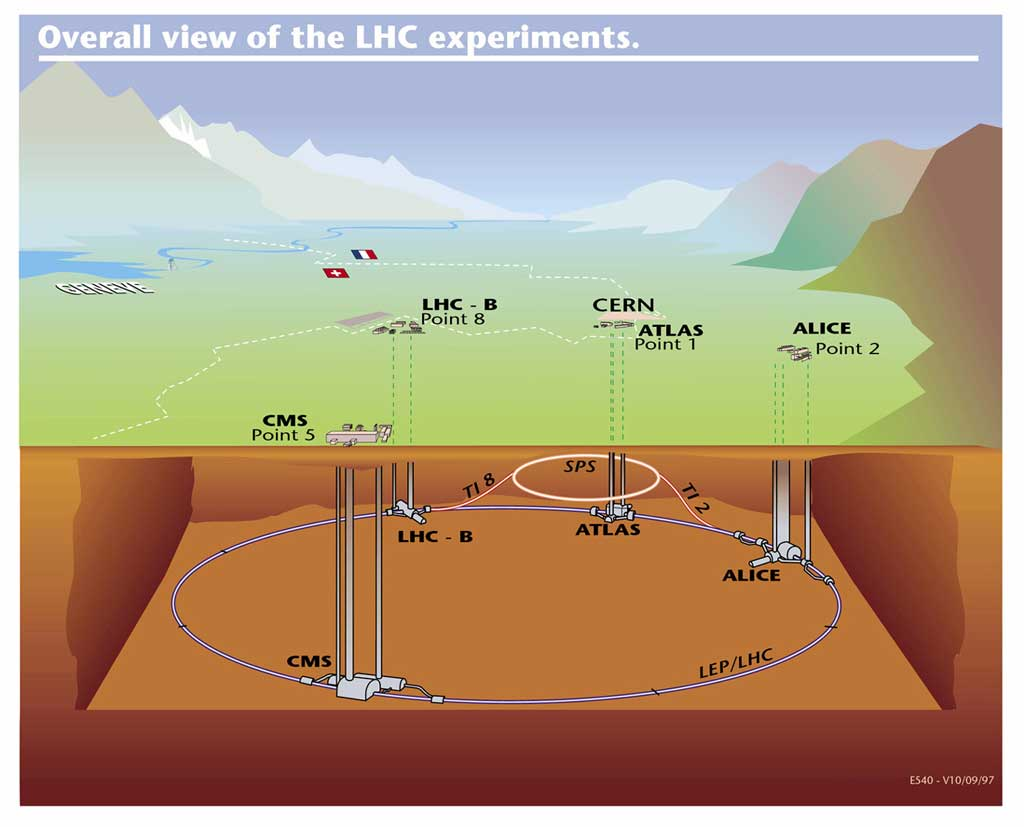
\includegraphics[width=0.8\textwidth]{Figures/detector/LHCdesign}
  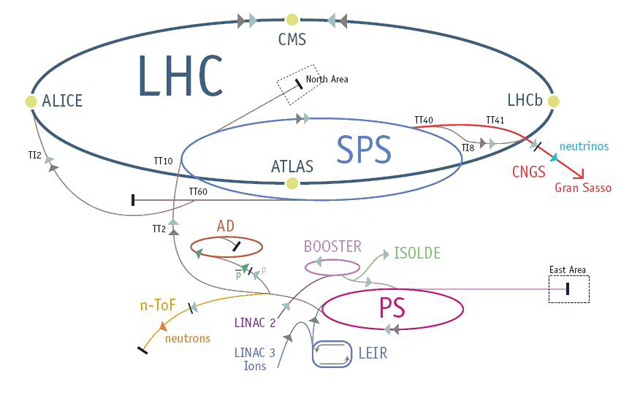
\includegraphics[width=0.8\textwidth]{Figures/detector/lhc}
  \caption{The ~\LHC accelerator ring, showing the locations of the four main experiments at the four collision points.
}
  \label{fig:LHC}
  \end{center}
\end{figure}

Interaction points are at the centre of four large particle detectors, shown in Figure~\ref{fig:LHC}:
\ac{ALICE}~\cite{Aamodt:2008zz}, 
\ac{ATLAS}~\cite{Aad:2008zzm}, 
\ac{CMS}~\cite{Chatrchyan:2008aa} and 
\ac{LHCb}~\cite{Alves:2008zz}.
They act to identify particles produced as a result of a pp or PbPb bunch crossing through a combination of tracking and calorimetry, in order to reconstruct and measure physical processes, to test currently accepted theories and search for new physics.

%running in Run 1

%%%%%%%%%%%%%%%%%%%%%%%%%%%%%%%%%%%%%%%%%%%%%%%%%%%%%%%%%%%%%%%%%%%%%%%%%%%%%%%%%%%%%%%%%%%%%%%
%   _____ __  __  _____ 
%  / ____|  \/  |/ ____|
% | |    | \  / | (___  
% | |    | |\/| |\___ \ 
% | |____| |  | |____) |
%  \_____|_|  |_|_____/ 
%                       
%%%%%%%%%%%%%%%%%%%%%%%%%%%%%%%%%%%%%%%%%%%%%%%%%%%%%%%%%%%%%%%%%%%%%%%%%%%%%%%%%%%%%%%%%%%%%%%

\section{The CMS Detector}
\label{sec:CMS}

The \ac{CMS} detector is a general purpose particle detector situated at Point 5 on the \ac{LHC} ring, designed to carry out many different measurements for various physics goals.
Close to 4$\pi$ solid angle reconstruction with 
efficient particle identification and reconstruction allows measurements of photons, muons, electrons, taus, hadronic showers and missing transverse momentum.
%It is therefore very well suited to the search for new physics, and direct production of \ac{SUSY}, in many different forms.
%Here, we focus on the search for new physics, particularly using the monojet final state.
%
A diagram of \ac{CMS} is shown in Figure~\ref{fig:CMS}. It is 21.6~\m long, 14.6~\m in diameter and weighs 12500~T. 
It consists of different sub-detectors, each of which measures a different particle or property, 
and is built around a central 12.5~m long 4~\T superconducting solenoid magnet and its iron return yoke.
%
\ac{CMS} consists of a barrel region, containing the solenoid, and endcaps to extend the forward and backward coverage.

%
The different sub-detectors are arranged in an onion structure.
%
Closest to the beam line is the silicon tracking system.
A very highly resolution pixel detector lies closest to the interaction region, followed by a granular strip detector.
Charged particle momenta measurements are made using the curvature of tracks in the uniform magnetic field provided by the solenoid, as well as measurements of displaced vertices and impact parameters which are essential for identifying heavy flavor decays. 
%
Energy measurements are provided by the calorimeters, which lie outside the tracker; the \ac{ECAL} and \ac{HCAL}. 
The highly granular \ac{ECAL} consists of 70,000 transparent lead tungstate crystals. 
%which cause electromagnetic showers and produce scintillation light 
As electrons and photons pass through, they cause electromagnetic showers in the crystals, which produce scintillation light.
% allowing position and energy measurements. 
%Scintillation light produced in the crystals is collected by photodetectors and used to infer the incident particle energy.
%
The sampling \ac{HCAL} consists of slabs of brass interleaved with plastic. 
Incident hadrons shower when passing through the absorber (brass), causing scintillation light to be produced in the active material (plastic) as the shower passes through.
%
Scintillation light produced in the crystals, or plastic, is collected by photodetectors and used to infer the incident particle energy and position.
%
The solenoid lies outside the \ac{HCAL} and provides a 3.8~\T axial magnetic field.
%
Embedded in the iron return yoke of the magnet sits the muon system. 
Three different types of muon detectors are used to identify muons and make momentum and charge measurements over a large kinematic range.
%
More information on the CMS detector can be found in Ref.~\cite{Chatrchyan:2008aa}.

%
% Crucial to the successful operation of \ac{CMS} is the trigger. 
% The pp interaction cross section is 100~\mb, while for example, the W boson production cross section is some 6 orders of magnitude less than this, and the rare physics processes that \ac{CMS} was built to search for, such as Higgs boson and \ac{SUSY} production, many times smaller still.
% The \ac{LHC} delivers an unprecedented high instantaneous luminosity so that such rare physics processes occur, but this also implies that the vast majority of the collisions result in `uninteresting' physics: namely \ac{QCD} processes.
% It would be impossible to record such high volumes of data that comes out of \ac{CMS}, some PB s$^{-1}$, and not useful to do so.
% Therefore, a very efficient method of recording those events that appear `interesting'  
% is necessary, to reduce the 40~\MHz event rate to a more manageable 100~\Hz.
% The two-tier trigger system fulfills this role, via a hardware based online \ac{L1} an software based offline \ac{HLT} and is described in Section~\ref{sec:CMStrig}.

%

%%%%%%%
% Inside the solenoid and closest to the beam line is the tracking system.
% In the uniform magnetic field provided by the solenoid, charged particles leave curved tracks 
% in the component silicon pixels and strips, under the influence of the Lorentz force.
% Momenta measurements are made by measuring the curvature of these tracks.
% %
% The next subsystems out are the calorimeters: the \ac{ECAL} and \ac{HCAL}. 
% Consisting of absorber materials which cause electromagnetic and hadron showers, they totally absorb a particle, prompting scintillation light proportional to its energy in the active material. 
% An energy measurement is made by measuring the scintillation light and inferring the energy of the incident particle.
% %
% Finally, embedded in the return yoke of the magnet sit the muon systems. 
% Muons are relatively long lived, heavier and therefore more penetrating than other particles,
% so require detectors further away from the interaction point. 
% Three different types of muon detectors, interleaved with the steel return yoke of the solenoid, are used to identify muons and make momentum and charge measurements over a large kinematic range.
% %
% More information on the CMS detector can be found in Ref.~\cite{Chatrchyan:2008aa}.

%picture
\begin{figure}[htbp]
  \begin{center}
  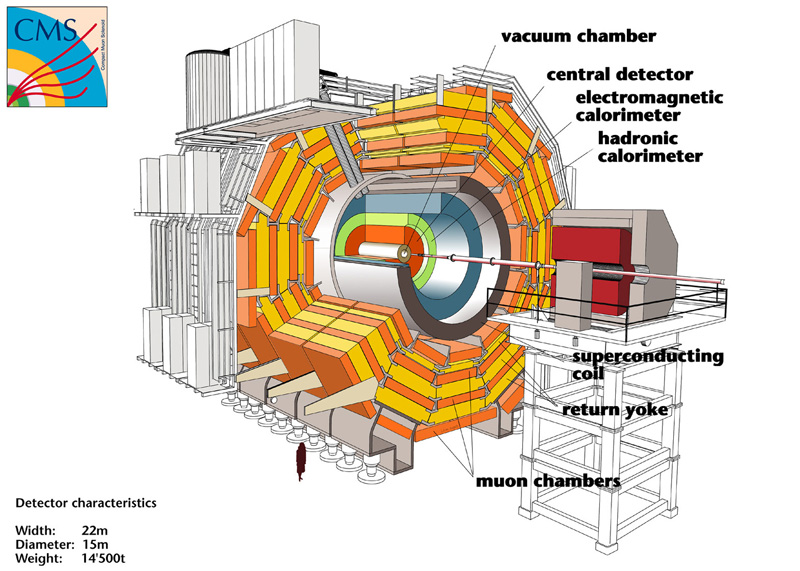
\includegraphics[width=0.8\textwidth]{Figures/detector/CMSlabelled}
  \caption{The \ac{CMS} detector, with the main subsystems labelled.
}
  \label{fig:CMS}
  \end{center}
\end{figure}

%coordinate system
\ac{CMS} uses a right-handed coordinate system: the $x$-axis points south towards the centre of the \ac{LHC} ring, the $y$-axis points vertically upwards and the $z$-axis is in the direction of the beam, where positive $z$ is to the West.
More natural is the coordinate system defined in terms of $r$, $\phi$ and $\theta$.
The azimuthal angle $\phi$ is measured from the $x$-axis in the $xy$ plane, where the radial component is denoted $r$. The polar angle $\theta$ is defined in the $rz$ plane, and the pseudorapity 
\begin{equation}
\eta = - \ln \tan (\theta /2).
\end{equation}
Convention is that the position of a particle is described in terms of $\eta$ and $\phi$, where $\eta = 0$ is along the $y$-axis and $\eta = \infty $ is along the beam direction; and $-\pi < \phi < \pi$. The distance between particles is commonly described in terms of the variable $\Delta R = \sqrt{\Delta\phi^2+\Delta\eta^2}$.

The \ac{LHC} is a hadron collider, and as such, collides non-fundamental particles. 
Inelastic collisions with large momentum transfer can occur between component quarks and gluons, however in a single bunch crossing there will also be many low energy, elastic, soft scatters, 
as well as the remnant part of any protons that have had a hard collision. 
As a result, the forward and backward directions are highly populated environments and therefore difficult to instrument due to high occupancy and radiation damage. 
\ac{CMS} has endcaps to extend the detector coverage at high $\eta$, however it is not possible to reconstruct the momentum of a single interaction in the direction of the beam.   
Additionally, interesting physics is a result of a hard collision, where energy is available for the creation of new particles. It can be characterized by the amount of energy in the transverse ($xy$) plane.
For these reasons, particle energy and momenta are described only in the transverse plane, where conservation laws can be applied.
By conserving energy and momentum in the transverse plane, any imbalance can be assigned to a particle leaving the detector without any trace; for example from a neutrino, or, from new physics processes such as \ac{DM} production
A nearly hermetic detector (with close to 4\pi coverage in solid angle) allow excellent particle reconstruction and measurements of missing transverse energy, the `tell-tale' sign of new physics, and make \ac{CMS} perfectly suited to searching for physics beyond the \ac{SM}.

%%%%%%%%%%%%%%%%%%%%%%%%%%%%%%%%%%%%%%%%%%%%%%%%%%%%%%%%%%%%%%%%%%%%%%%%

\subsection{The Tracking System}
The tracker is designed for precise and efficient measurement of charged particle trajectories (and therefore position and momentum) as they emerge from the interaction point.
Additionally, reconstruction of any secondary vertices is crucial for identifying heavy flavor decays such as jets that originate from b-quarks.

The \ac{LHC} provides bunch crossings every 25 or 50~\ns, resulting in $\sim$ 20 pp interactions, giving rise to of order 1000 particles. 
All of these traverse the tracker. 
The granularity of the tracker must be such that one can determine which of the $\sim$ 20 pp vertices each of the particles come from, 
and the electronics fast enough that the information is sent on in time for the next bunch crossing to arrive.
With such high particle fluxes, the tracker is also subject to a huge amount of radiation damage.
These conditions must be dealt with using the least amount of material possible in order to limit multiple scattering, photon conversion, bremsstrahlung and nuclear interactions.
To meet such criteria, and to have an estimated lifetime of 10 years, the tracker is constructed entirely from silicon.

The tracker consists of an all silicon pixel and strip detector.
Measuring 5.8~\m in length and 2.5~\m in diameter, with a total active area of 200~\msq, it surrounds the interaction region.
%pixel
The pixel detector has three layers in the barrel, at radii of 4.4~\cm, 7.3~\cm and 10.2~\cm. In the endcaps, there are two disks at distances $z=\pm 34.5, \pm 46.5~\cm$.
%strip
The strip detector has a length of 5.8~\m and a diameter of 2.4~\m, and is composed of four subsystems: the \ac{TIB}, \ac{TOB}, \ac{TID} and \ac{TEC}. The \ac{CMS} tracker geometry is shown in Figure~\ref{fig:CMStracker}.

%picture
\begin{figure}[htbp]
  \begin{center}
  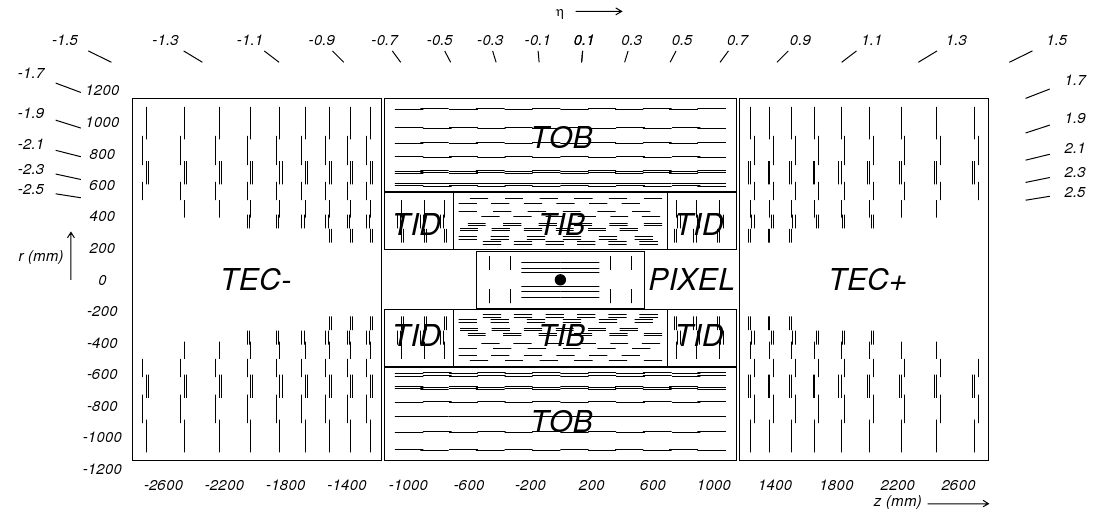
\includegraphics[width=0.9\textwidth]{Figures/detector/fig_cmstracker}
  \caption{The \ac{CMS} tracker, shown in the $rz$ plane. The pixel detector is shown at the centre of the tracker, closest to the interaction region (shown by the black dot), and the strip detector surrounds it. The different subsystems of the strip detector are shown. Taken from Ref.~~\cite{Chatrchyan:2008aa}.
}
  \label{fig:CMStracker}
  \end{center}
\end{figure}


%The resolution of a track is described in terms of five parameters
The energy resolution of the tracker is shown in Figure~\ref{fig:CMStrackerRes}, 
for samples of single muons with \pt of 1, 10 and 100~\GeV. 
For a 100\GeV muon, the resolution is 1-2\% up to $|\eta| = 1.6$. 
Lower momentum objects have a better energy resolution as their tracks have increased curvature.

%picture
\begin{figure}[htbp]
  \begin{center}
  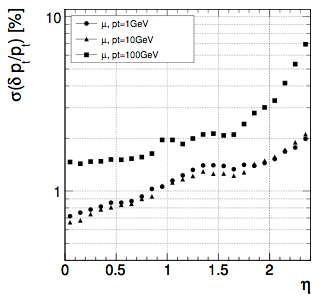
\includegraphics[width=0.3\textwidth]{Figures/detector/cmstrackerRes}
  \caption{The energy resolution as a function of $|\eta|$ for \ac{CMS} tracker, shown for single muons with \pt = 1, 10 and 100~\GeV. 
}
  \label{fig:CMStrackerRes}
  \end{center}
\end{figure}
%%%%%%%%%%%%%%%%%%%%%%%%%%%%%%%%%%%%%%%%%%%%%%%%%%%%%%%%%%%%%%%%%%%%%


\subsection{The Electromagnetic Calorimeter}
High resolution photon and electron position and energy measurements are provided by the lead tungstate (PbWO$_{4}$) crystal \ac{ECAL}, which covers pseudorapidty up to $|\eta|<3$.
It is made up of the \ac{EB}, covering the range $0<|\eta|<1.479$,
and the \ac{EE}, covering the range $1.479<|\eta|<3$.

Both fast response times (80\% of scintillation light is emitted in 25~\ns) and radiation hardness are required from the \ac{ECAL}, motivating the choice of material.
In addition, it is very dense (8.28~g$\cm^{-1}$), has a short radiation length ($X_{0} = 0.89~\cm$), and small Moli\`{e}re radius (2.2~\cm), making it well suited to a compact, fine granularity calorimeter.
Arranged in a quasi-projective geometry, 61,200 crystals in the barrel and 7,324 crystals in the endcaps are tapered in shape and angled at 3\deg to ensure that particle trajectories avoid cracks between them.
Barrel crystals have a front face of $22 \times 22$~mm$^{2}$ and a length of 23~\cm, corresponding to 25.8~$X_{0}$. 
Endcap crystals have a front face of $28.6 \times 28.6$~mm$^{2}$ and length corresponding to 24.7~$X_{0}$.
Electromagnetic showers are therefore expected to be contained within one crystal length, so only a single layer of crystals is needed. 
A preshower detector is place in front of the endcaps, with a thickness of $3X_{0}$, in the range $1.653<|\eta|<2.6$, in order to distinguish between single photons and photon pairs resulting from neutral pion decay. 
The \ac{ECAL} geometry is shown in Figure~\ref{fig:CMSecal}.

%picture
\begin{figure}[htbp]
  \begin{center}
  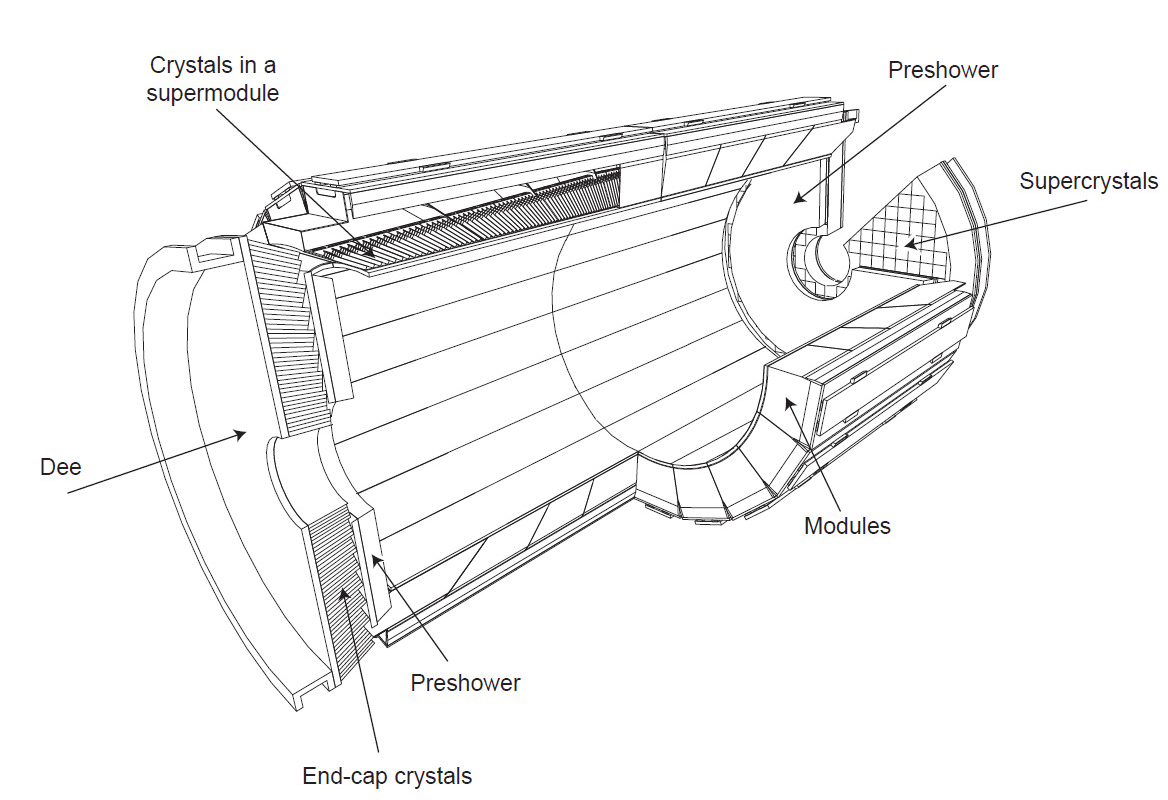
\includegraphics[width=0.7\textwidth]{Figures/detector/cmsECAL}
  \caption{Geometric view of the \ac{CMS} \ac{ECAL}. Barrel crystals are arranged in modules and supermodules, and endcap crystals arranged in supercrystals. Also shown is the preshower detector.
}
  \label{fig:CMSecal}
  \end{center}
\end{figure}

The very dense material PbWO$_{4}$ causes incident photons and electrons to shower. 
Resulting pair produced electrons and positrons, and radiated photons, cause scintillation light in the transparent, polished crystals. 
The amount of light produced is proportional to the incident particle energy, and is collected by an \ac{APD} on the end of each crystal in the barrel, and a \ac{VPT} in the endcaps. \textcolor{red}{[check if use these acronyms again]}
These photodetectors also have to be radiation hard and operate successfully in the 3.8~\T magnetic field, while providing significant amplification to signal.
Both the crystal and photodetector performance has a strong temperature dependence, so the \ac{ECAL} is kept at a constant temperature of 18\deg via a water cooling system, and is stable to $\pm0.05~\deg$C.

%energy resolution
The energy resolution of the \ac{ECAL} can be parametrised using the following equation:
\begin{equation}
\left(\frac{\sigma}{E}\right)^{2} = \left(\frac{S}{\sqrt{E}}\right)^{2} + \left(\frac{N}{E}\right)^{2} + C^{2},
\end{equation}
%laser calibration
where $S$ is due to stochastic scattering, $N$ is due to noise and $C$ is the constant term. Measurements in test beam are shown in Figure~\ref{fig:CMSecalRes}, where the terms were found to be: $S = 2.8\%$, $N=0.12~\GeV$ and $C = 0.30\%$. 

\begin{figure}
  \begin{center}
  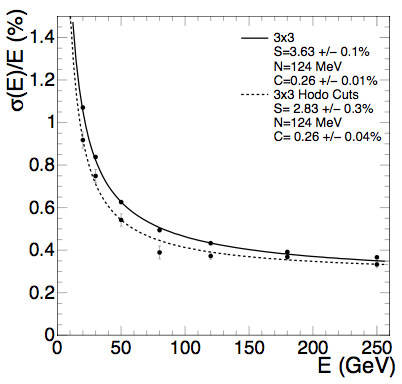
\includegraphics[width=0.5\textwidth]{Figures/detector/EcalRes.png}
  \caption{The energy resolution of an \ac{ECAL} supercrystal, measured in a test beam. The lower set of points along the dashed line correspond to the energy measured in an array of 3$\times$3 crystals, where events fall within a 4$\times$4~\mm region in the central crystal. 
}
  \label{fig:CMSecalRes}
  \end{center}
\end{figure}

%%%%%%%%%%%%%%%%%%%%%%%%%%%%%%%%%%%%%%%%%%%%%%%%%%%%%%%%%%%%%%%%%%%%%


\subsection{The Hadronic Calorimeter}
The \ac{HCAL} provides complementary energy measurements of hadronic showers, crucial for measuring jets and missing transverse energy.
It is a sampling brass calorimeter, built from alternating layers of large, absorbing brass plates, interleaved with scintillating plastic tiles arranged in trays. 
Sitting within the bore of the solenoid, the \ac{HB} covers pseudorapidity $|\eta|<1.3$,
and the \ac{HE} on each side enclose $1.3<|\eta|<3$.
To attain a most hermetic detector, there is also a \ac{HF}, which extends coverage right up to $|\eta|<5.2$.

The quality of the \ac{HCAL}'s measurements is dictated by the fraction of the hadronic shower that passes through the scintillator; the plastic must be thick enough to catch the majority of the shower.
This demand for radial extension is at odds with the location of the \ac{HCAL}, from the outer edge of the \ac{ECAL} at $r=1.77~\m$, and the inner edge of the solenoid at $r=2.95~\m$.
Providing a compromise, an outer hadronic calorimeter, \ac{HO}, is placed outside of the vacuum tank of the magnet and supplements the \ac{HB}.
Using the solenoid coil as absorber material, it can identify late starting showers, providing sufficient containment for 11.8 interaction lengths.% ($\lambda_{L}$).
Five rings of \ac{HO} are arranged along the $z$-axis of the detector, where the central ring at $\eta=0$ has two layers at $r=3.82~\m$ and $4.07~\m$, and the rest have a single layer at $r=4.07~\m$. 
Figure~\ref{fig:CMShcal} shows the geometry of the \ac{HCAL}.

%picture
\begin{figure}[htbp]
  \begin{center}
  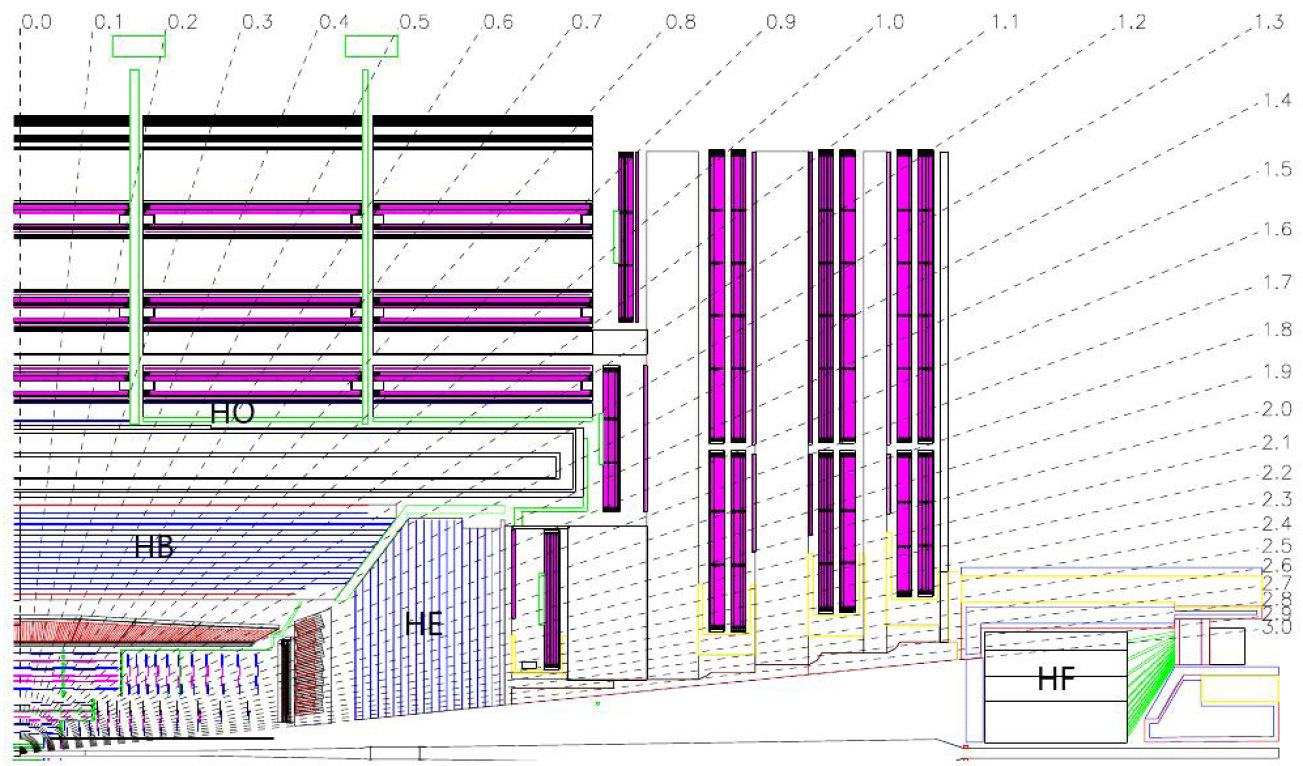
\includegraphics[width=0.9\textwidth]{Figures/detector/cmsHCAL}
  \caption{Longitudinal view of the \ac{CMS} \ac{HCAL}. Locations of the \ac{HB}, \ac{HO}, \ac{HE} and \ac{HF} are shown with values of $\eta$. The purple regions represent the muon detectors which further restrict the volume of the \ac{HO}.
}
  \label{fig:CMShcal}
  \end{center}
\end{figure}

Hadron showers are created in the brass absorber plates, through nuclear interactions in the material, and the plastic scintillator tiles produce blue-violet light when the shower passes through. 
It is read out using wavelength shifting fibres, sending the now green light down transparent fibres to \ac{HPD} which produce an electrical signal proportional to the incident hadron energy.
The first layer of plastic tiles are placed in front of the first absorber plate in order to sample the incoming shower as it develops in the material between the \ac{ECAL} and the \ac{HCAL}.
The final layer of scintillator placed after the final brass plate to catch any late developing showers.
There are 70,000 plastic scintillator tiles in the \ac{HB} and 20,916 tiles in the \ac{HE}.

The \ac{HF} uses a different technology in order to cope with the much harsher environment in which it is situated.
With an average energy of 760~\GeV deposited in the \ac{HF} per pp collision at LHC design energy, peaking at the highest rapidity point closest to the beam line, radiation hardness and occupancy requirements demand alternative materials.
Steel absorber plates are embedded with scintillating quartz fibres, which act to detect the Cherenkov light emitted by charged particles in the shower. 
It is therefore most sensitive to the electromagnetic component of the shower.

The energy resolution of the \ac{HCAL} was measured in pion beam tests. The energy response and 
resolution are shown in Figure~\ref{fig:CMShcalRes}, and the fractional energy response is parametrised
as 
$\frac{\sigma}{E} = \frac{120\%}{\sqrt{E}} \oplus 6.9\%$.

%picture
\begin{figure}[htbp]
  \begin{center}
  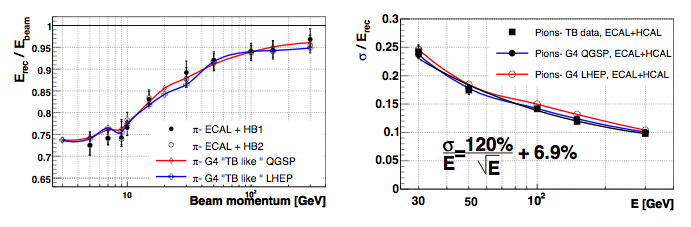
\includegraphics[width=0.9\textwidth]{Figures/detector/HCALres}
  \caption{The raw energy response (left) and fractional energy resolution (right) as a function of energy, for pions, in team beam data.
}
  \label{fig:CMShcalRes}
  \end{center}
\end{figure}

%%%%%%%%%%%%%%%%%%%%%%%%%%%%%%%%%%%%%%%%%%%%%%%%%%%%%%%%%%%%%%%%%%%%%%%%%%%%%%%%%%%%%%%%%%%%%%%

\subsection{The Muon System}
%do i need this
Muons are a powerful tool for recognising signs of interesting physics. 
%Many SUSY models predict excesses of muon decays, for example $B_{s}\rightarrow\mu\mu$, 
%and the Higgs decay $\H \rightarrow \Z\Z$ where both \Z decay to two muons has been called the ``golden plated'' channel.
A relatively easy experimental signature to identify, muons can provide excellent 2- or 4-particle mass resolutions 
as, due to their larger mass, they do not suffer large radiative losses (as electrons do).
%They are therefore of vital importance to the physics programme at \ac{CMS}, such that they take the middle word of the experiment's name.
Muon reconstruction is therefore a central design feature. 
Embedded in the iron flux-return yoke of the solenoid, the muon system combines three methods of gaseous detection to identify, carry out high resolution momentum measurements, and trigger events, up to $|\eta|<2.4$. 
Figure~\ref{fig:CMSmuonSys} shows a cross section of one of the five wheels that make up the barrel section of muon system; there are also two planar endcaps which sit at either end of the detector and enclose it.

%picture
\begin{figure}[htbp]
  \begin{center}
  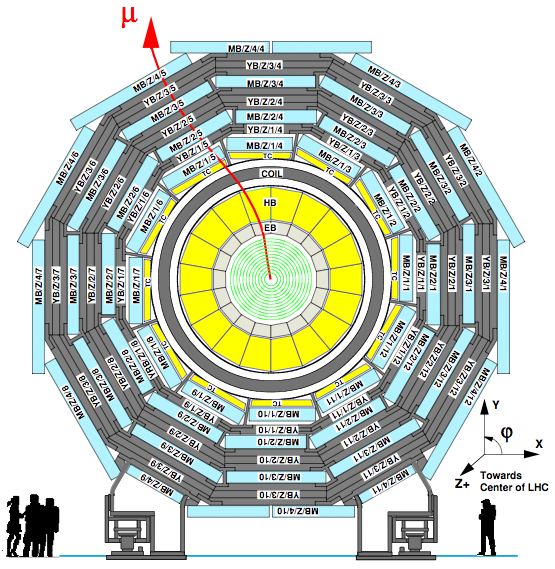
\includegraphics[width=0.7\textwidth]{Figures/detector/muonSystems}
  \caption{One of the 5 wheels of the barrel of the \ac{CMS} muon system. Gaseous detectors are embedded in the iron return yoke of the solenoid; due to the small residual magnetic field in the barrel, \ac{DT}s are used.
}
  \label{fig:CMSmuonSys}
  \end{center}
\end{figure}



In the barrel ($|\eta|<0.9$), magnetic flux is concentrated in the iron return yoke so the residual field is very small.
There is also a low muon rate and neutron induced background, so \ac{DT} chambers are used.
In the endcaps ($0.9<|\eta|<2.4$), magnetic field and muon rate are much higher, so \ac{CSC} are used instead; 
they have a faster response time, higher granularity and better radiation hardness.
Both the \ac{DT} and \ac{CSC} have excellent position resolution.
An additional system of \ac{RPC} in both the barrel and endcaps provide an independent signal which has good time resolution (and poorer position resolution) and serves as a trigger.


By combining information from the tracker, and from either the \ac{DT} or \ac{CSC} and \ac{RPC}, \ac{CMS} has excellent muon reconstruction. 
Precise momentum resolution is achieved for the kinematic range, from 10~\GeV to $>500~\GeV$, shown in  
Figure~\ref{fig:CMSmuonRes}. 

%picture
\begin{figure}[htbp]
  \begin{center}
  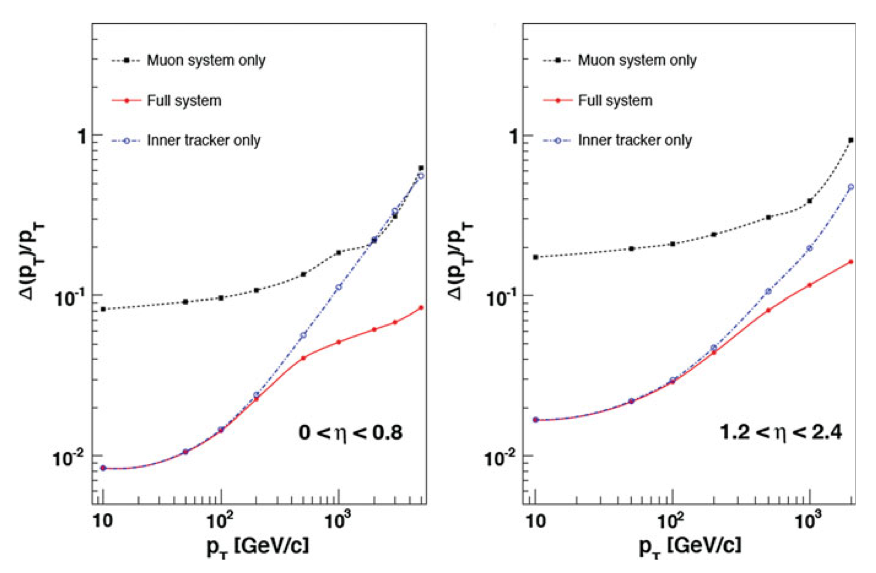
\includegraphics[width=0.8\textwidth]{Figures/detector/CMSmuonRes}
  \caption{Muon transverse momentum resolution, shown as a function of muon \pt in the barrel (left) and the endcaps (right). The resolution of the tracker and muon system is shown, and the enhancement gained by combining the information.
}
  \label{fig:CMSmuonRes}
  \end{center}
\end{figure}

%%%%%%%%%%%%%%%%%%%%%%%%%%%%%%%%%%%%%%%%%%%%%%%%%%%%%%%%%%%%%%%%%%%%%%%%%%%%%%%%%%%%%%%%%%%%%%%
%  ________      ________ _   _ _______   _____  ______ _____ ____  
% |  ____\ \    / /  ____| \ | |__   __| |  __ \|  ____/ ____/ __ \ 
% | |__   \ \  / /| |__  |  \| |  | |    | |__) | |__ | |   | |  | |
% |  __|   \ \/ / |  __| | . ` |  | |    |  _  /|  __|| |   | |  | |
% | |____   \  /  | |____| |\  |  | |    | | \ \| |___| |___| |__| |
% |______|   \/   |______|_| \_|  |_|    |_|  \_\______\_____\____/ 
%                                                                  
%%%%%%%%%%%%%%%%%%%%%%%%%%%%%%%%%%%%%%%%%%%%%%%%%%%%%%%%%%%%%%%%%%%%%%%%%%%%%%%%%%%%%%%%%%%%%%%

\newpage
\section{Event Reconstruction} \label{sec:CMSreco}

It is by piecing together the information from the various subsystems of the \ac{CMS} detector that, for example, a track in the tracking system, or an energy deposit in the \ac{HCAL}, can be attributed to a particle or ``physics object''. 
Figure~\ref{fig:CMSslice} shows a slice of the whole detector with each of the main physics objects traversing it: muons, electrons, photons, and charged and neutral hadrons.
Each of these leaves a different signature.
Charged particles leave tracks in the silicon tracker, curved under the influence of the magnetic field.
Electrons and photons cause electromagnetic showers, leaving energy deposits in the \ac{ECAL}.
Hadrons penetrate further, showering and leaving energy deposits in the \ac{HCAL}. 
Muons are the only visible particles to reach the muon system, where they leave tracks.

%picture
\begin{figure}[htbp]
  \begin{center}
  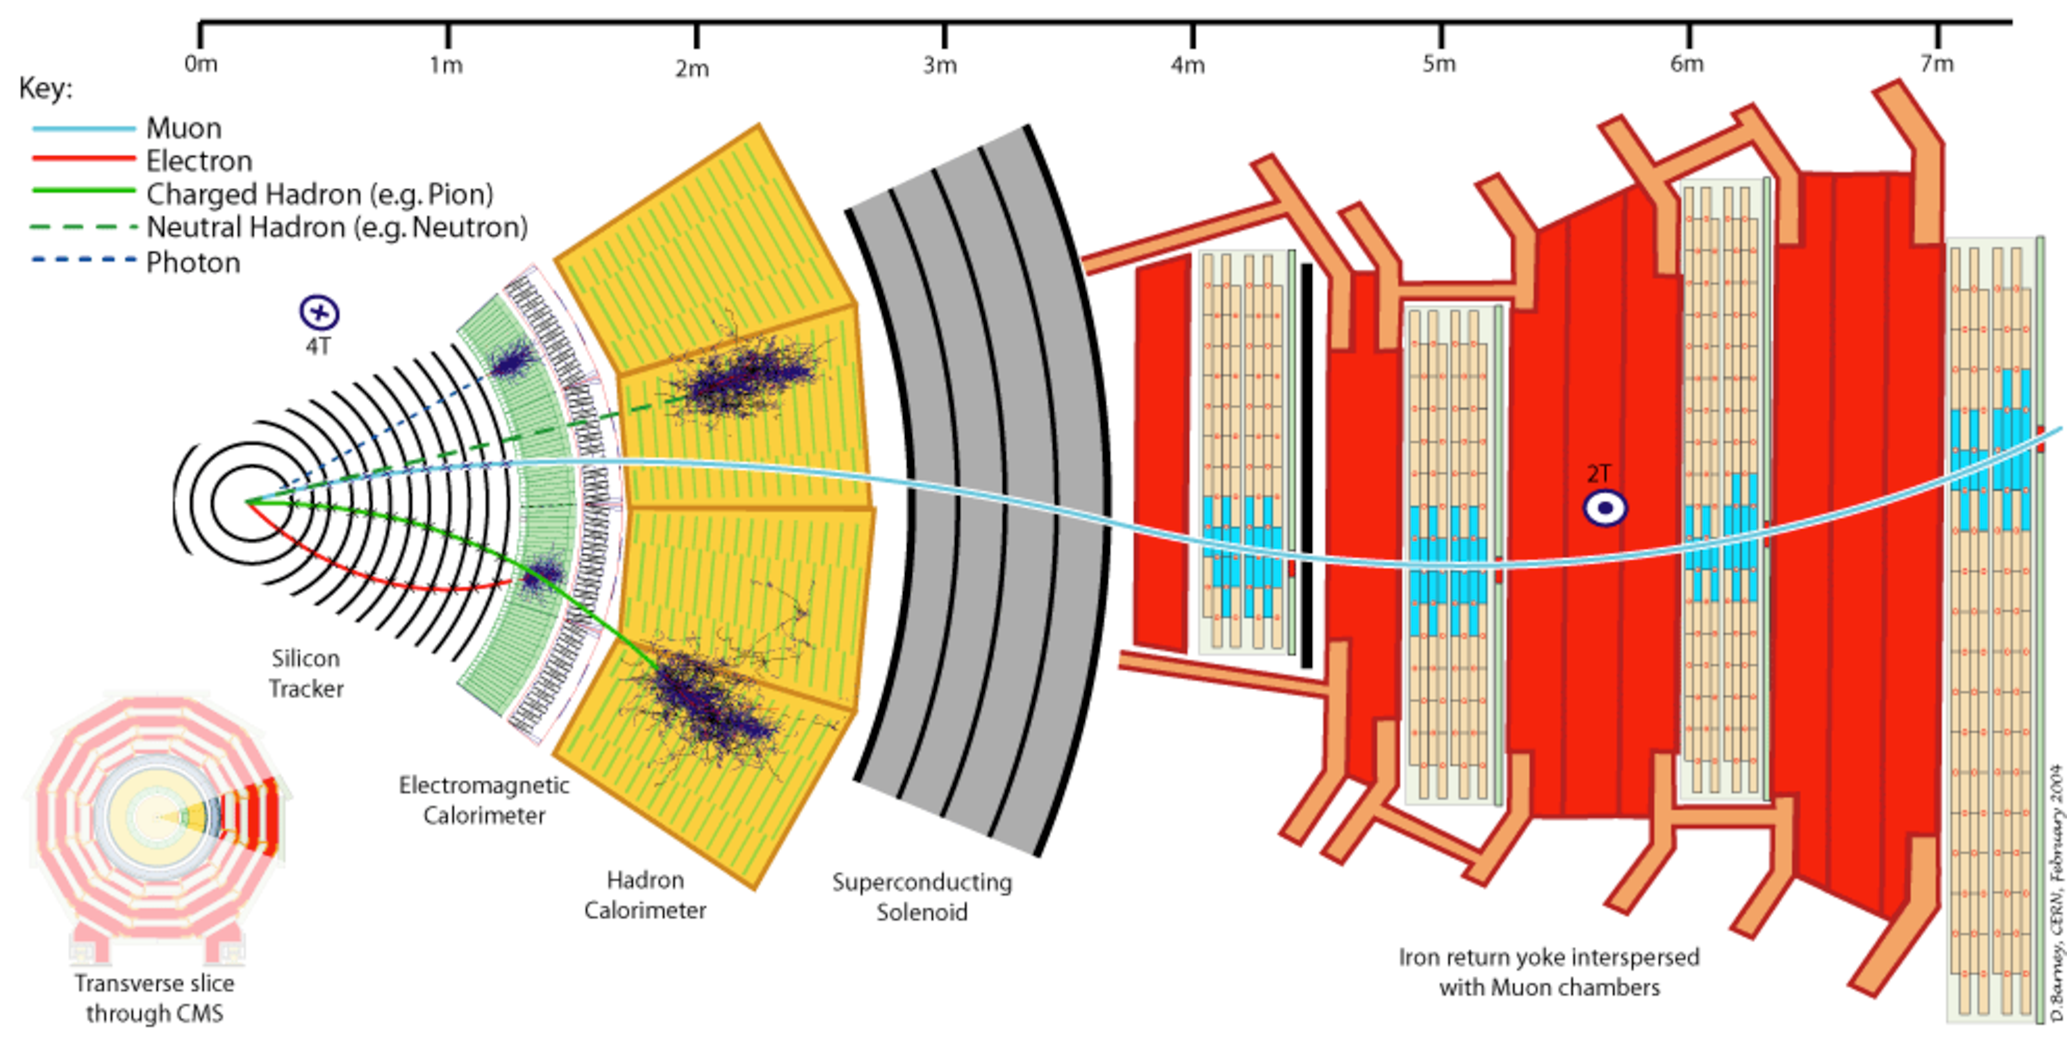
\includegraphics[width=0.9\textwidth]{Figures/detector/CMS_Slice.pdf}
  \caption{A slice of the \ac{CMS} detector is shown, with various particles, or physics objects, traversing it. By combining information from each of the subdetectors, each of the particles produced in an event can be identified and the whole event reconstructed.
}
  \label{fig:CMSslice}
  \end{center}
\end{figure}

Particles can then be identified by combining tracking information with data from the calorimeters and muon system.
If there is an energy deposit in the \ac{ECAL}, the only way to distinguish between a photon or electron is by looking to see if there are hits in the tracker, leading to the position of the electromagnetic shower in the calorimeter. 
Similarly, the momentum measurement of the electron, determined using the curvature of the track it leaves (also used to reconstruct its charge), can be combined with the energy measurement made using the amount of scintillation light produced in the \ac{ECAL} to get a better resolution.
If there is no track leading to the electromagnetic shower, a photon is instead reconstructed.
Hadronic showers in the \ac{HCAL} due to charged and neutral incident hadrons can also be distinguished by their tracks.
A muon will leave the tell-tale sign of hits in the tracker, and hits in the outer muon chambers, where position, momentum and charge measurements from both ensure the initial track in the silicon tracker matches up to the track in the muon system. Dual measurements also lead to enhanced resolution.


Below is a summary of the object reconstruction most relevant to the physics analysis described in Chapter~\ref{chap:sus13009}. 
More information can be found in Ref.~\cite{TDRVOL1}.


\subsection{Jets}
Copious numbers of quarks and gluons are produced during pp collisions in \ac{CMS}, a consequence of the huge \ac{QCD} cross section.
Through the strong interaction they fragment and immediately hadronise, and a spray of hadrons is produced in the direction of an initial quark or gluon.
Various algorithms have been developed in order to group the spray of hadrons into a ``jet'', and assign an energy, direction and transverse momentum to it.

In the analysis presented in this thesis (and in general at \ac{CMS}), the anti-k$_{\mathrm{t}}$ algorithm~\cite{bib:akjets} is used with a distance parameter, $R = 0.5$.
It behaves like an idealised cone algorithm, using a distance parameter to cluster particles into cone shapes, with a radius $R$. Soft particles are clustered with nearby hard particles rather than with themselves, leading to conical jets, which --- crucially --- are resilient to soft radiation on the boundary of the cone.
Likewise, the area of the jet is unaffected by soft radiation on the boundary, and is equal to $\pi R^{2}$. 
These features make the anti-k$_{\mathrm{t}}$ algorithm the preferential jet algorithm at \ac{CMS}, due to its insensitivity to soft radiation that arises from sources such as \ac{PU}; see Figure~\ref{fig:antikT_PU}. 

%picture
\begin{figure}[htbp]
  \begin{center}
  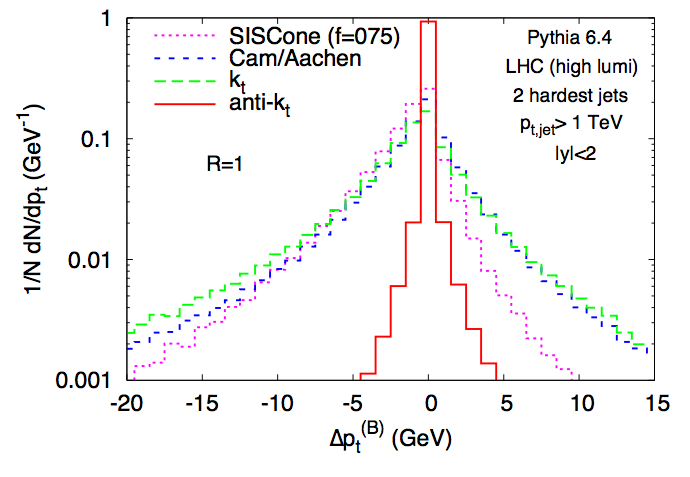
\includegraphics[width=0.7\textwidth]{Figures/detector/PUantiKT}
  \caption{The relative insensitivity of the anti-k$_{\mathrm{t}}$ algorithm to \ac{PU} is shown, compared to other common jet algorithms. The distribution of back reaction, corresponding to the net change in \pt to each of the two hardest jets (where each jet has $\pt>200~\GeV$), when adding \ac{PU}$\sim 25$ to the event, corresponding to \ac{LHC} running conditions in the next phase of data taking starting in 2015. Taken from~\cite{bib:akjets}.}
  \label{fig:antikT_PU}
  \end{center}
\end{figure}

Several types of jets exist at \ac{CMS}, in which the anti-k$_{\mathrm{t}}$ algorithm is given different inputs.
Calorimeter (Calo) jets use information from the calorimeter only.
\ac{ECAL} crystals are grouped in $5\times5$ arrays into ``towers'', which measure $0.087\times0.87$ in $\Delta\phi \times \Delta \eta$ space (in the barrel region) and are matched to aligning blocks of \ac{HCAL}.
The sum of the energy deposits in both layers of calorimeter are used as inputs to the jet algorithm, where towers are treated as massless and an $\eta$ dependent energy threshold has been placed on each tower to reduce the effect of instrumental noise. 

The \ac{PF} algorithm~\cite{PFT-09-001} creates a list of all stable particles in an event: photons, electrons, muons, neutral hadrons and charged hadrons.
Particle momentum, direction and type are determined using all of the subdetectors of \ac{CMS}, 
which, with its silicon tracker, highly granular \ac{ECAL} and strong magnetic field is ideally suited to the task.
The reconstruction of the fundamental constituents of a typical jet --- largely photons, charged hadrons and neutral hadrons --- uses charged particle tracks and calorimeter clusters, termed ``elements''.
A traversing particle is expected to give rise to one, or several elements arising from separate subdetectors. 
%For example, a charged hadron could make one charged particle track and a calorimeter cluster. 
To reconstruct a particle, these elements are therefore grouped into ``blocks'': links of one, two or three elements
that have arisen due to the same object.
Blocks can then be interpreted as individual particles, and the resulting list of reconstructed particle flow particles 
gives a global description of each event.
This list of particles is used as the input to the anti-k$_{\mathrm{t}}$ algorithm, producing \ac{PF} anti-k$_{\mathrm{t}}$ jets.

The energy of a typical jet consists of energy from charged particles (65\%), photons (25\%) and neutral hadrons (10\%).
Therefore, typically, 90\% of the jet energy can be reconstructed with good precision, utilising measurements from the high resolution silicon tracker and \ac{ECAL}. 
Only 10\% of the energy, arising from neutral hadrons, is reconstructed using the relatively poor resolution hadron calorimeter. 
Therefore, \ac{PF} jets, made of reconstructed particles, are much closer to jets made of simulated, \ac{MC} generated particles than those that rely just on calorimeter information alone (such as Calo jets), see Figure~\ref{fig:PFturnOns}.
\ac{PF} jets consequently have excellent position and energy resolution. 
Jet momentum resolution, defined as the ratio $(\pt^{\mathrm{rec}} - \pt^{\mathrm{gen}})/\pt^{\mathrm{gen}}$, (where ``rec'' is for reconstructed, i.e. \ac{PF} or Calo jets, and ``gen'' is for jets taken from simulation) 
is shown in Figure~\ref{fig:PFmomRes}.
It is because of the excellent performance of the \ac{PF} algorithm, as input to the anti-k$_{\mathrm{t}}$ that it is used most commonly across \ac{CMS} analyses, including in the analysis presented in this thesis.

%picture
\begin{figure}[htbp]
  \begin{center}
  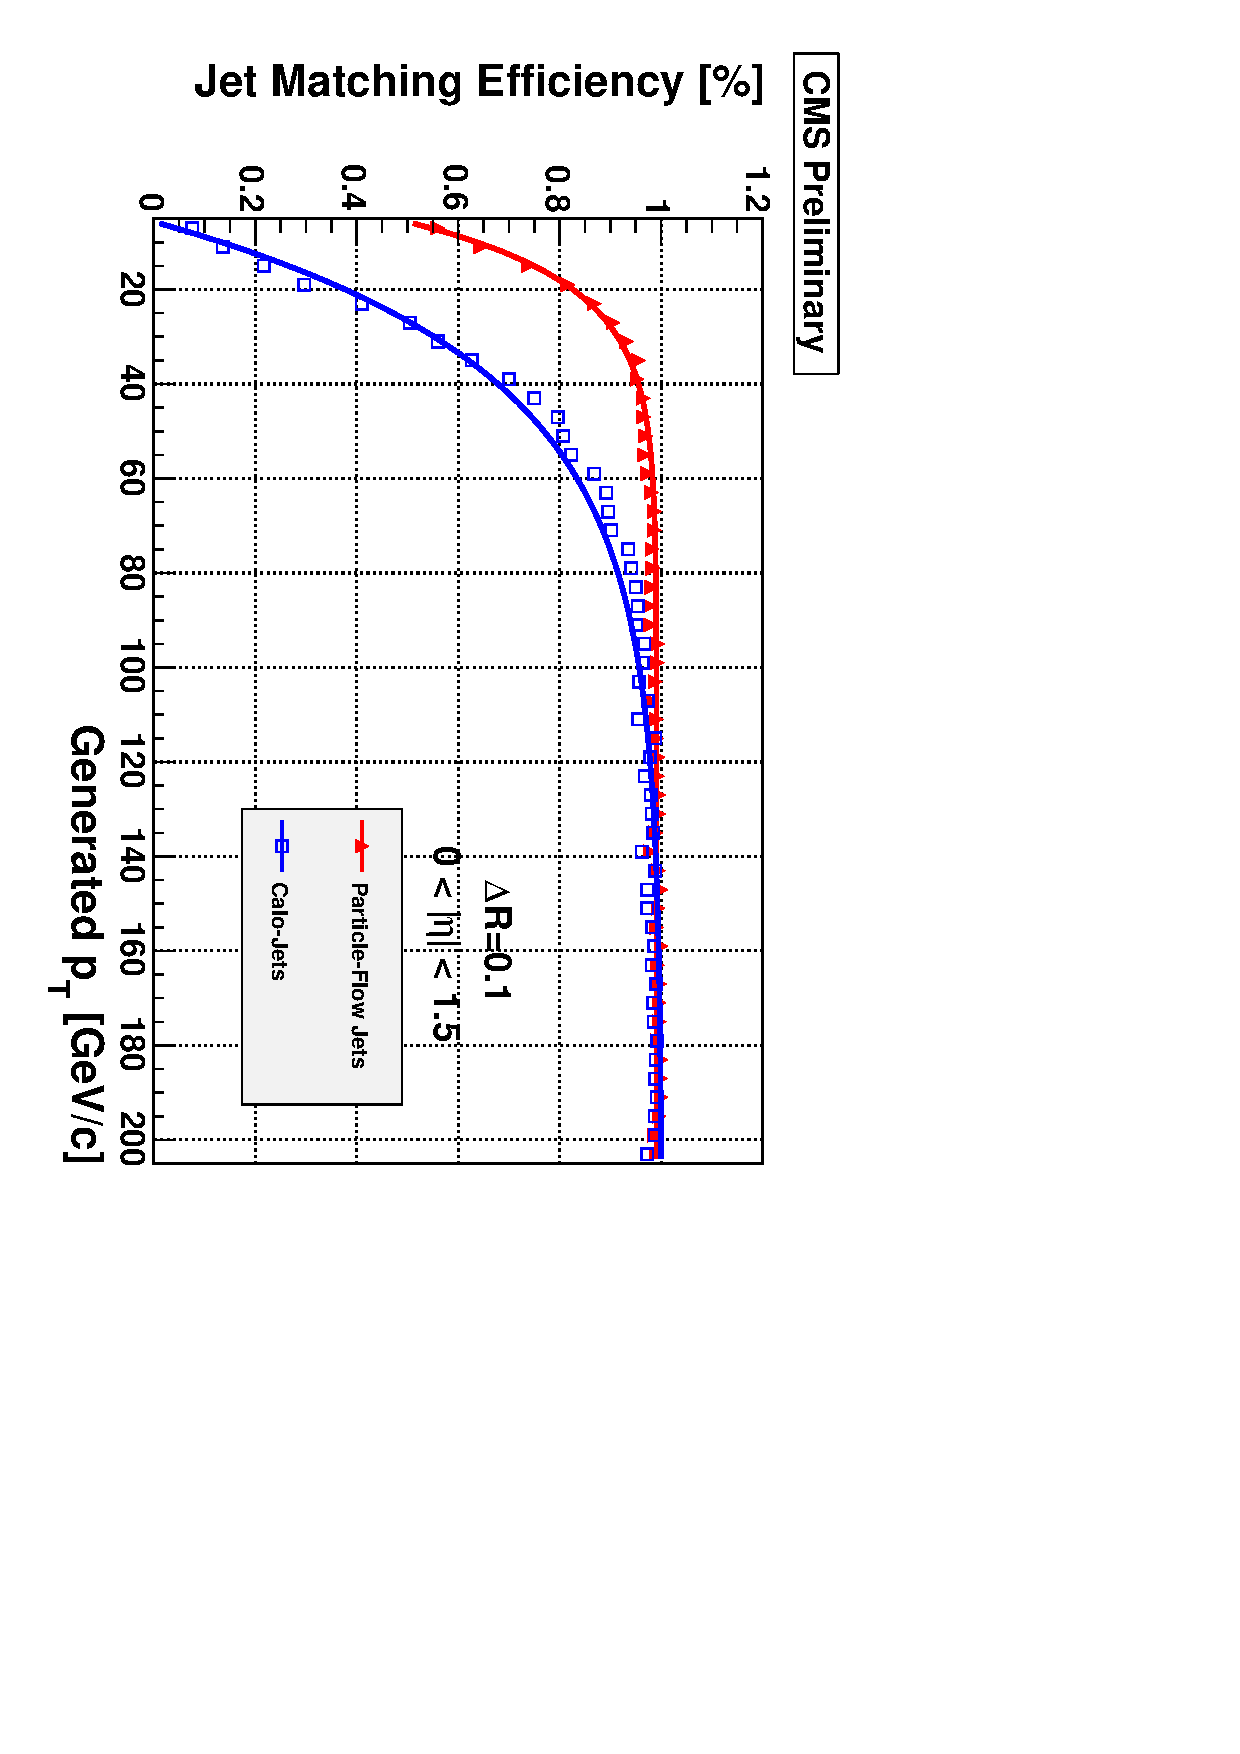
\includegraphics[width=0.33\textwidth, angle =90]{Figures/detector/PFjetvsCalo0p1}
  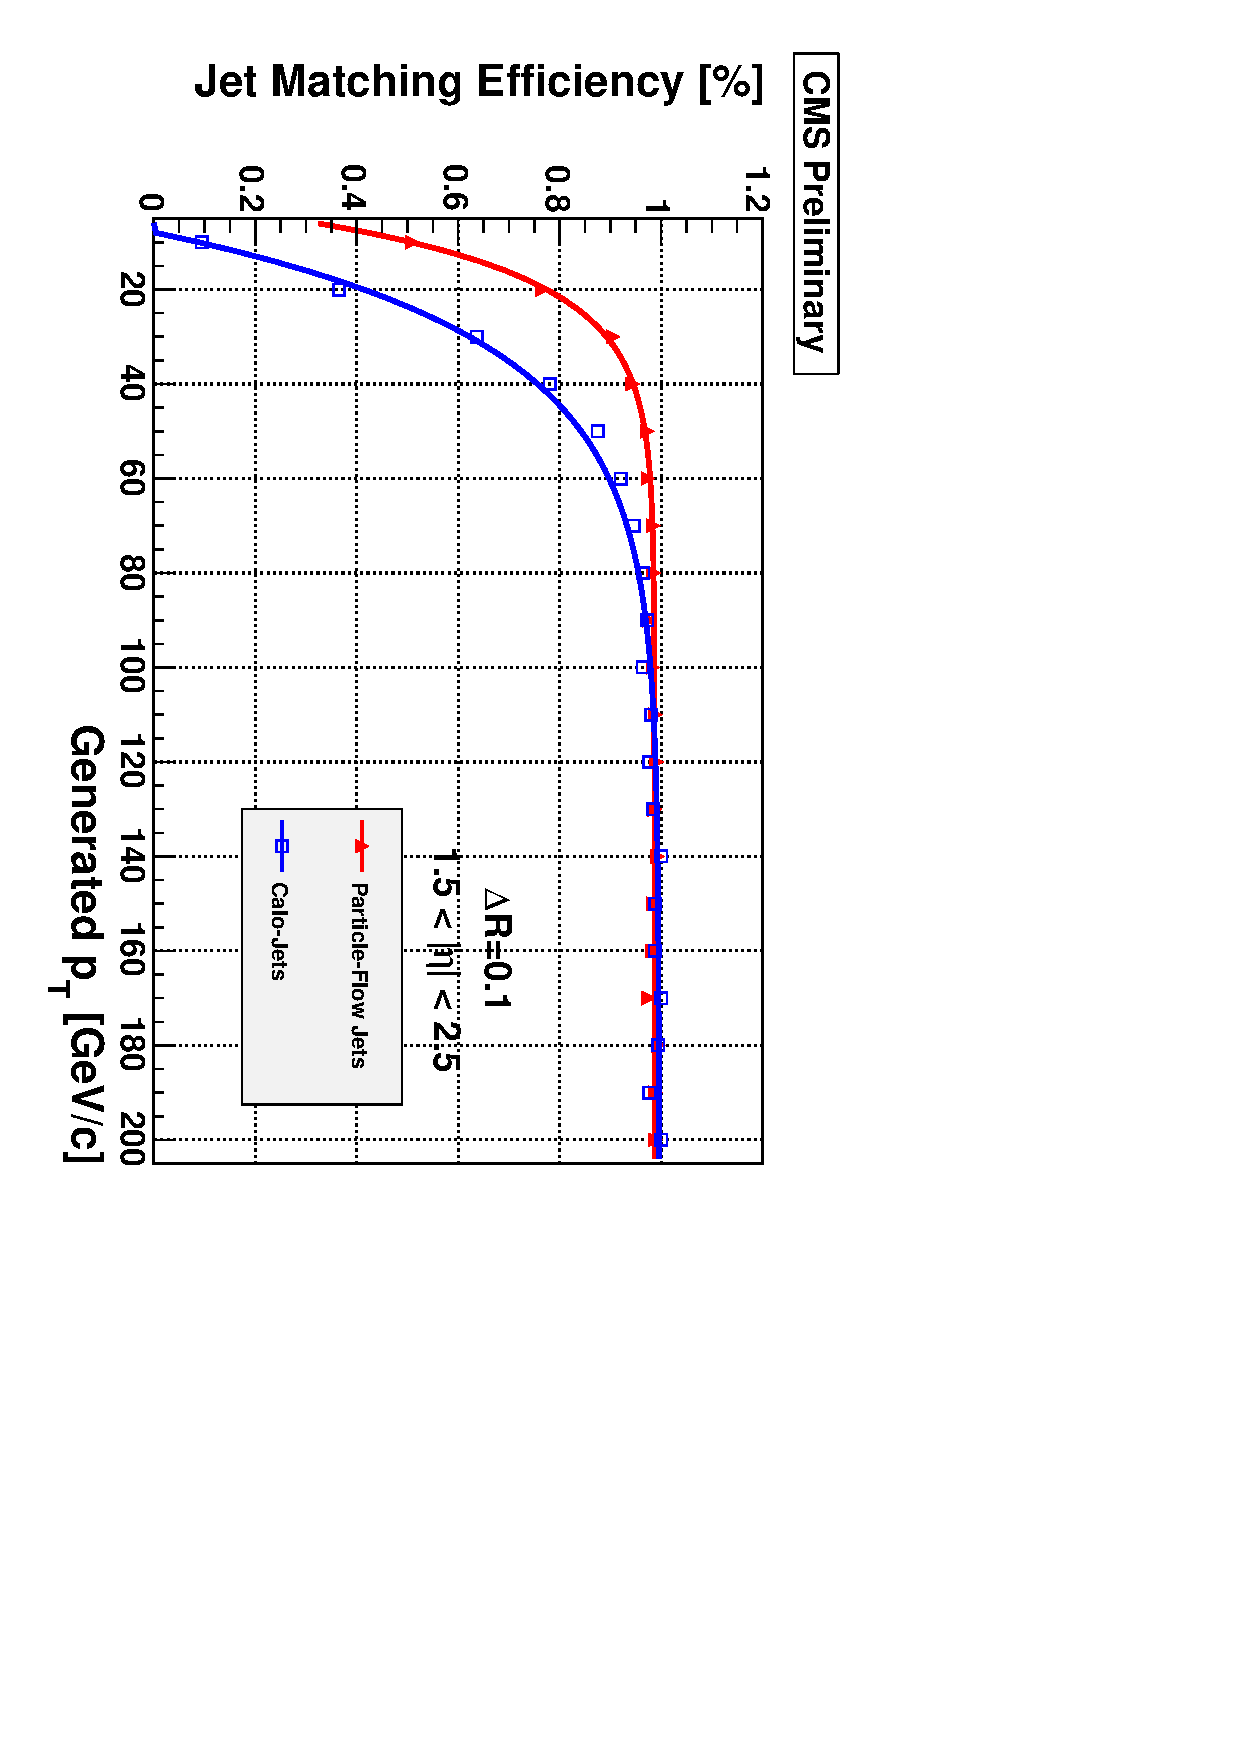
\includegraphics[width=0.33\textwidth, angle =90]{Figures/detector/PFjetvsCalo0p1end}
  \caption{The efficiency of \ac{PF} jets, and Calo jets, matched to generated jets in the barrel region (left) and the endcap (right), taken from~\cite{PFT-09-001}. The superior performance of \ac{PF} jets is evident because they are more efficiently matched to the generator, ``truth'' jets, at a lower \pt threshold: termed a sharper turn-on.}
  \label{fig:PFturnOns}
  \end{center}
\end{figure}

%picture
\begin{figure}[htbp]
  \begin{center}
  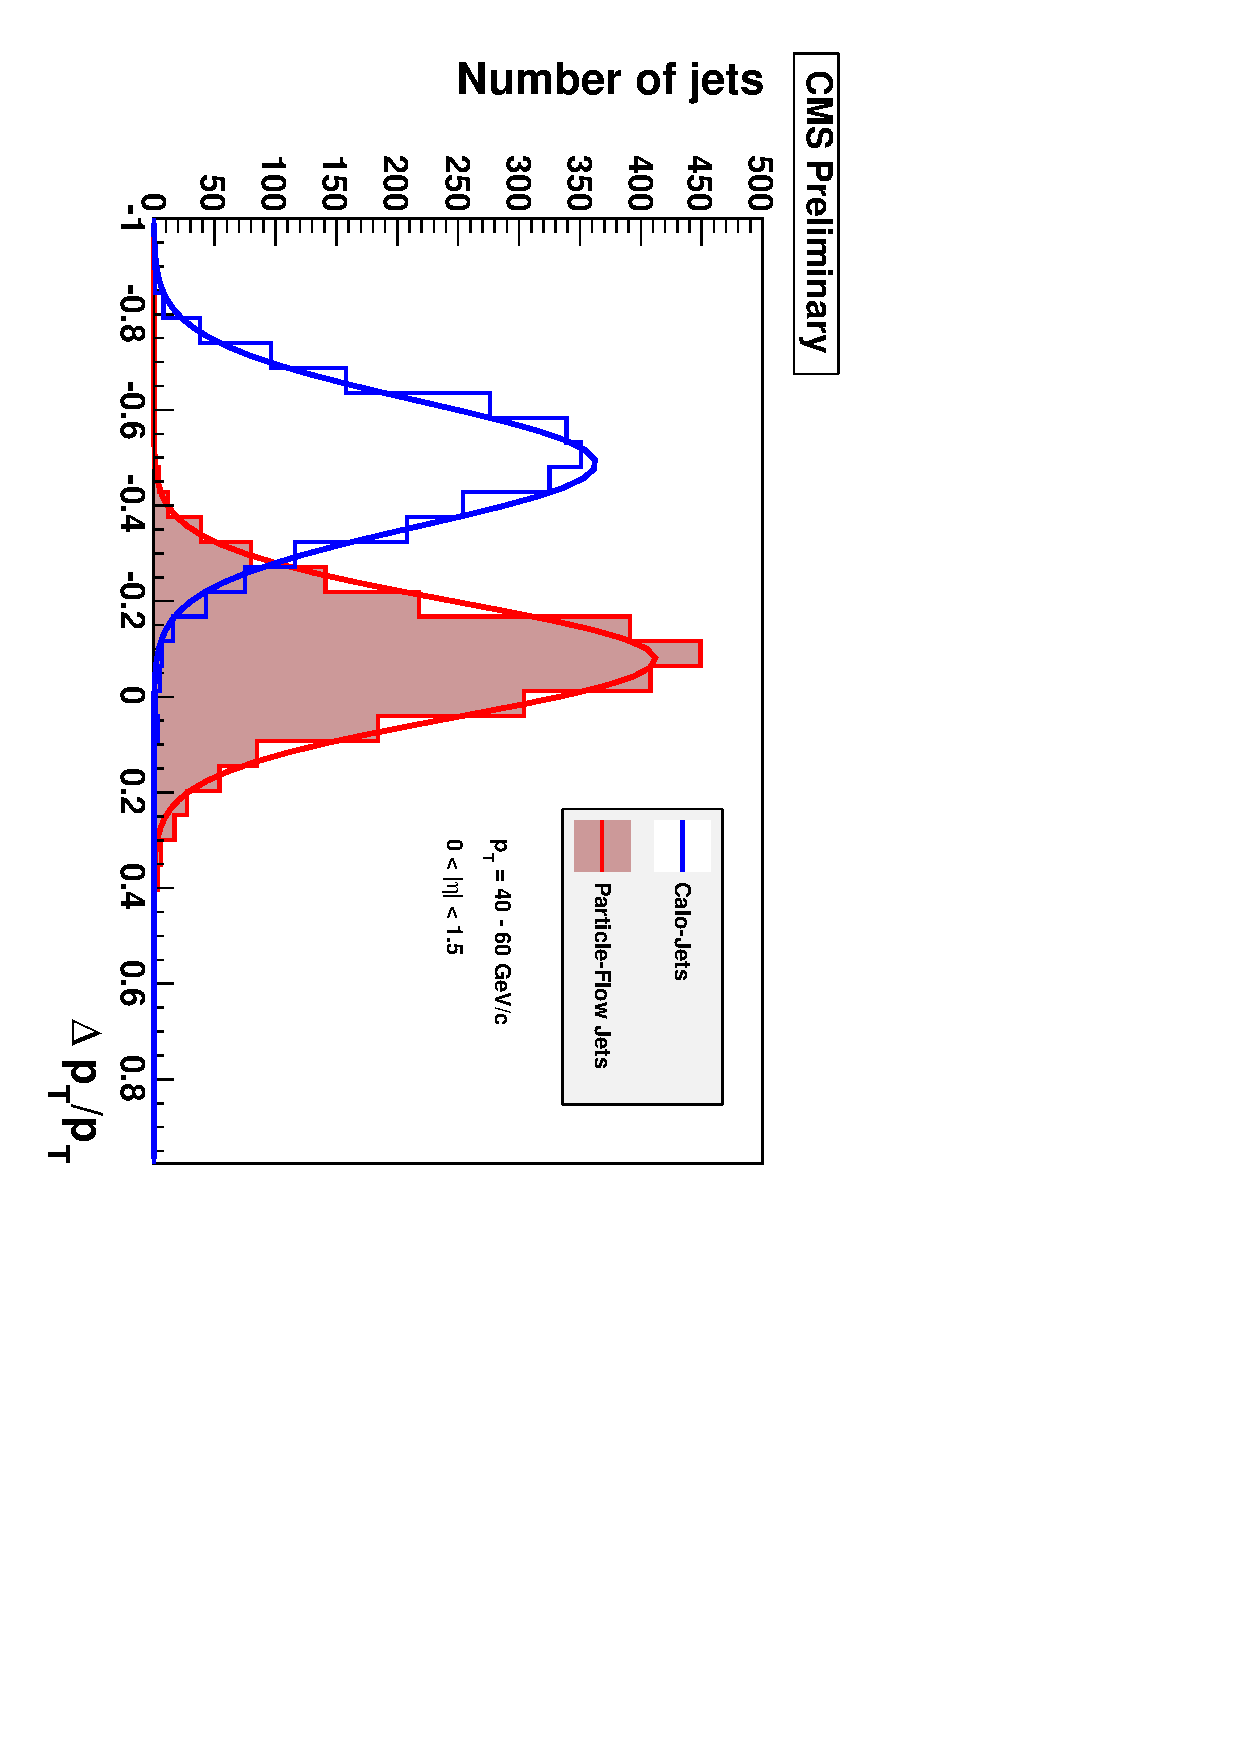
\includegraphics[width=0.33\textwidth, angle =90]{Figures/detector/MomResPFjetCaloJet_lowPt.pdf}
  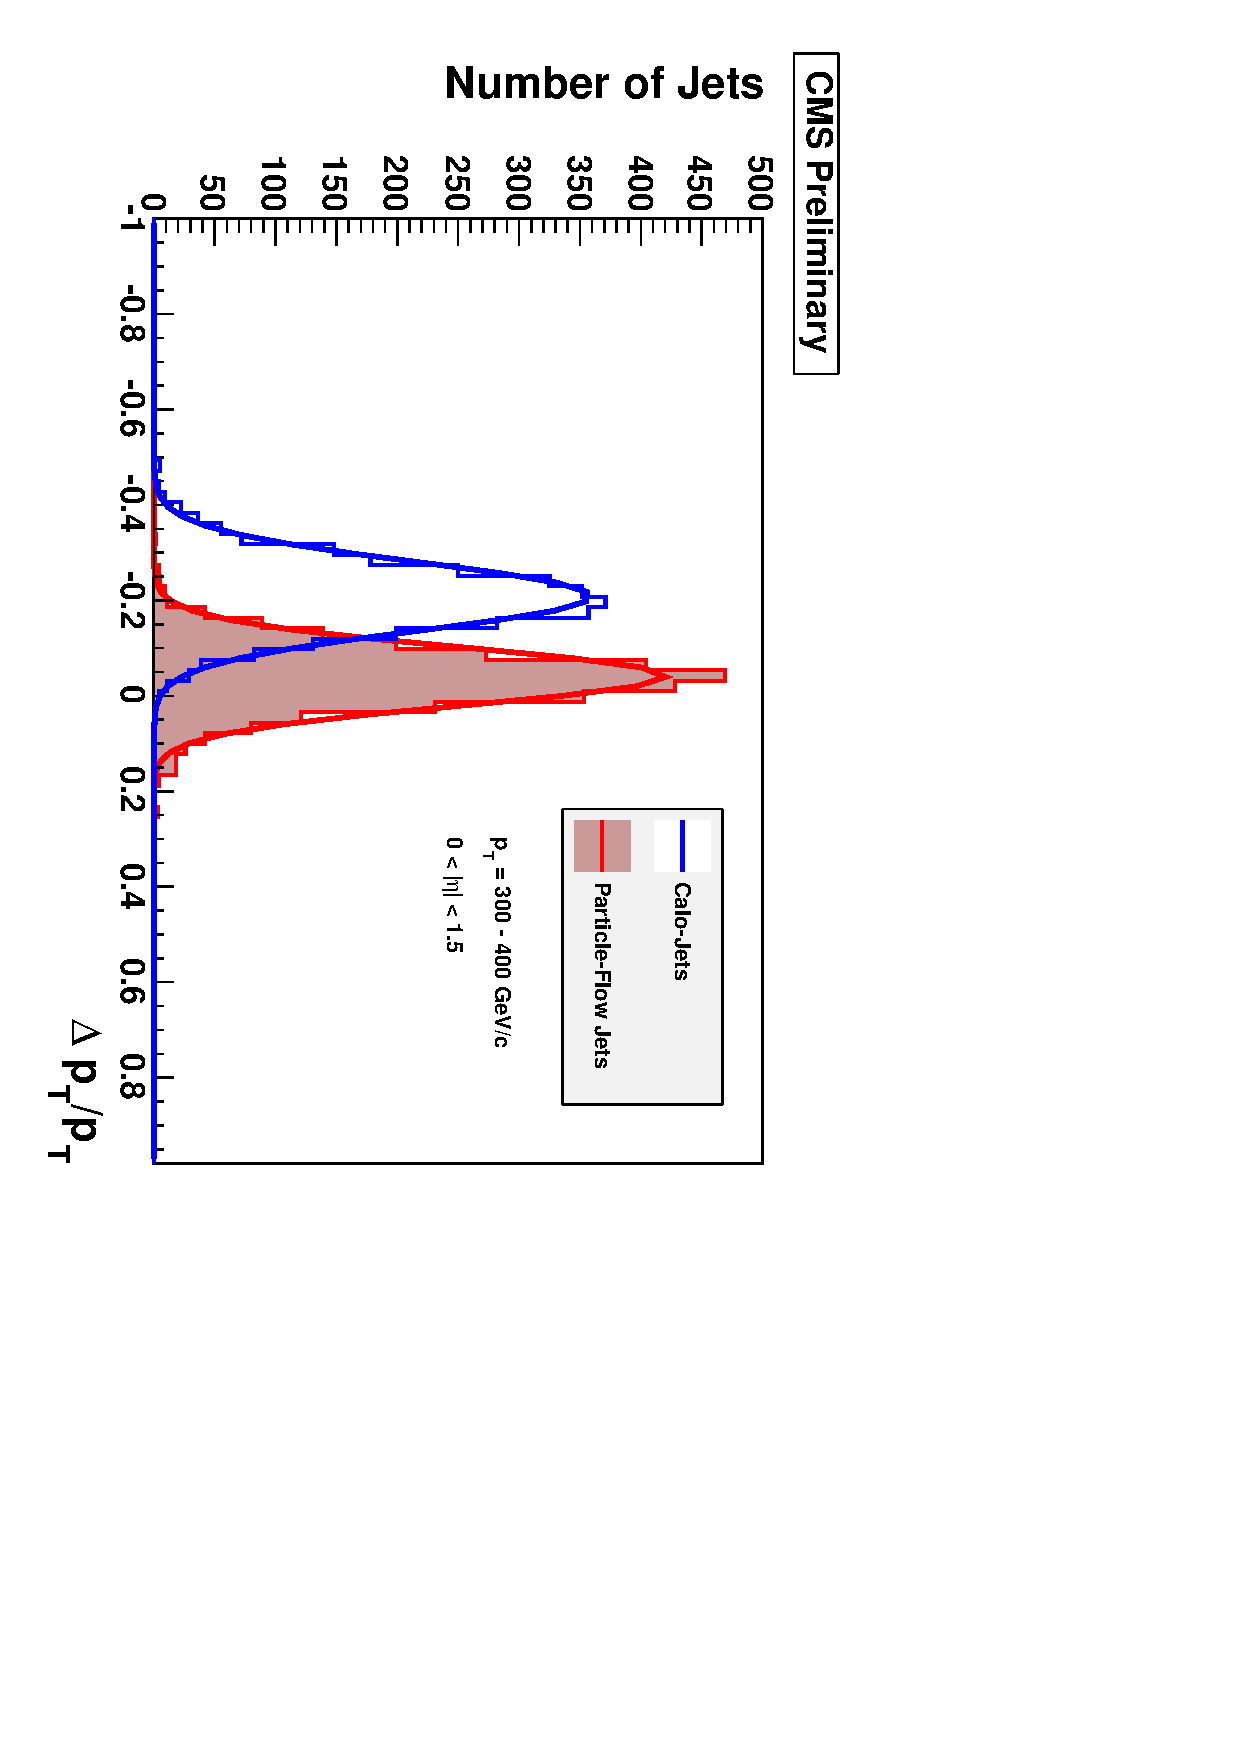
\includegraphics[width=0.33\textwidth, angle =90]{Figures/detector/MomResPFjetCaloJet_highPt.pdf}
  \caption{The momentum resolution, $(\pt^{\mathrm{rec}} - \pt^{\mathrm{gen}})/\pt^{\mathrm{gen}}$ of \ac{PF} jets, and Calo jets, for low energy jets ($40~\GeV<\pt<60~\GeV$) (left) and for high momentum jets ($300~\GeV<\pt<400~\GeV$) (right) in the barrel region, taken from~\cite{PFT-09-001}. Not only are the peaks sharper for \ac{PF} jets, meaning a smaller (and therefore better) overall momentum resolution, but it is also peaking much closer to zero, meaning the jet measurement is much closer to the generated jet momentum.}
  \label{fig:PFmomRes}
  \end{center}
\end{figure}


\subsection{Missing Transverse Energy}

As discussed in the previous sections, \ac{CMS} is nearly hermetic, has coverage up to $|\eta| = 5$ and excellent particle reconstruction; a very complete picture of each event is available. 
As such, is it very well suited to make measurements of weakly interacting particles, such as neutrinos, that do not leave any trace within any subsystem of the detector; and are only evident through an imbalance of transverse momentum.
New physics processes, such as R-parity conserving \ac{SUSY}, would also lead to signatures involving a large imbalance in transverse momentum as the weakly interacting \ac{LSP} exits the detector. \ac{DM} production would also lead to such a signature.
Measurements of missing transverse energy and momentum are therefore crucial to the search for new physics at \ac{CMS}, as they have been crucial in previous discoveries --- for example of the W boson~\cite{bib:Wdiscovery}, and in searches for other processes~\cite{Albajar:173124,Albajar:173125}. 

The missing transverse energy vector, $\METv$ is formed by adding the transverse energy vectors $\sum \ETv$ of all the particles formed in an event. The missing transverse energy vector $\METv = - \sum \ETv$, where $|\METv| = \MET = |\sum \ETv|$; i.e., it is equal in magnitude and opposite in direction to the total visible energy in the event.
In an analogous way to jets (and usually using such jets), $\MET$ can be built using various algorithms. 
Calorimeter (Calo) \MET, in the same way as Calo jets, is built from calorimeter information alone while
\ac{PF} \MET is calculated from all of the transverse energies of reconstructed particles in an event. 
In a similar way to the jet algorithms, a better resolution is achieved using the \ac{PF} algorithm over calorimeter information alone, see Figure~\ref{fig:PFMET}
However, because energy measurements of particle flow objects are driven by calorimeter resolution, particularly for large \ET objects, the improvement is less marked.
In the analysis presented in this thesis, \ac{PF} \MET is used, where any muons present have been removed from the  calculation. It therefore mimics Calo \MET, only with an enhanced resolution. 

%picture
\begin{figure}[htbp]
  \begin{center}
  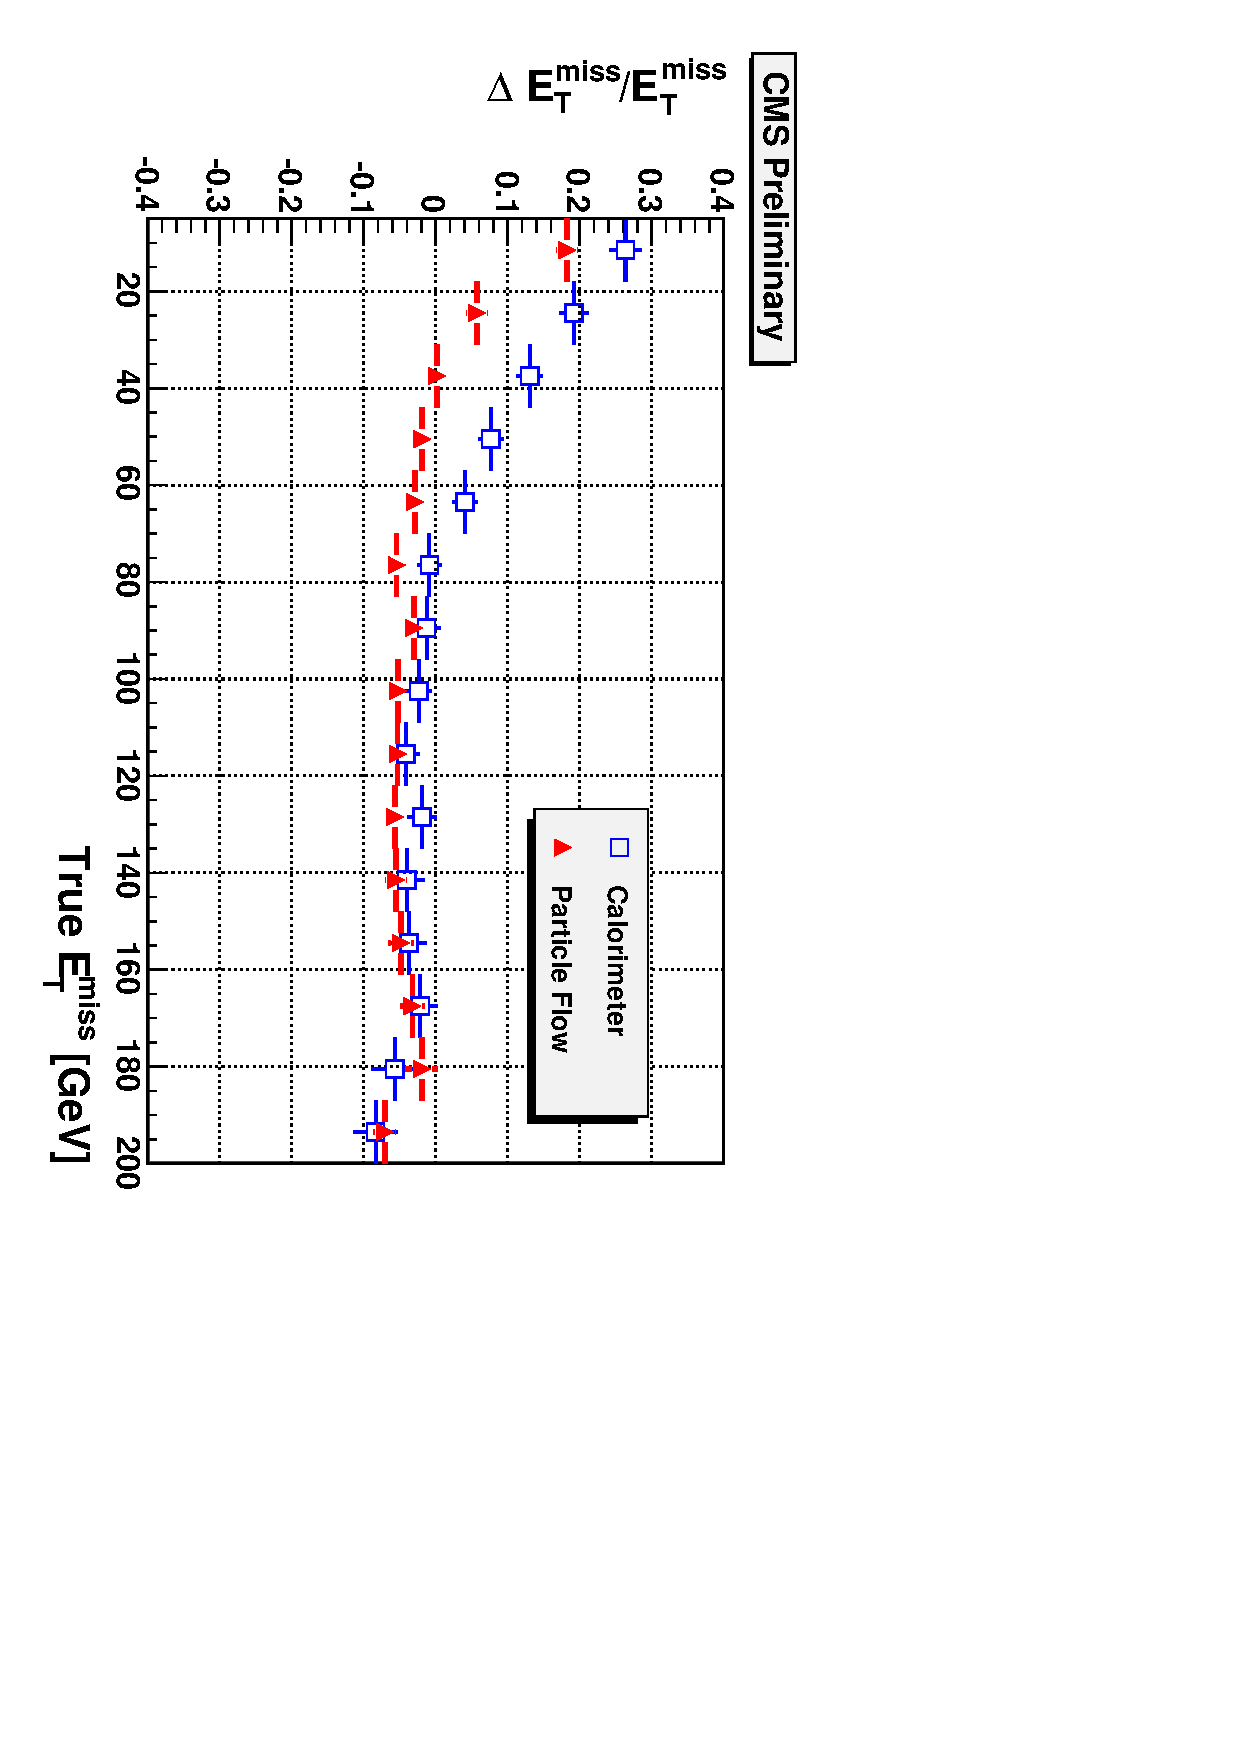
\includegraphics[width=0.53\textwidth, angle =90]{Figures/detector/METresPF.pdf}
  \caption{The momentum resolution, $(E^{\mathrm{miss}}_{T,rec} - E^{\mathrm{miss}}_{T,\mathrm{gen}})/E^{\mathrm{miss}}_{T,\mathrm{gen}}$ of \ac{PF} and Calo \MET, taken from~\cite{PFT-09-001}. An improved resolution is seen using the \ac{PF} algorithm, particularly at low values of \MET. At higher \MET values, energy measurements are dominated by the calorimeter resolution and values using the two different methods converge.}
  \label{fig:PFMET}
  \end{center}
\end{figure}

\subsection{Muons}

Muons are reconstructed using the muon systems and the tracker, and the reconstruction algorithms use the concept of ``regional reconstruction''. 
On the basis of an input or seed from the muon systems, the software only reconstructs the part of the tracker from which the muon causing the seed could originate.
This means that only a very small part (typically a few percent) of the tracker volume must be processed to reconstruct a muon; thereby speeding up the procedure and reducing the CPU power necessary to process an event.

Muon reconstruction has three stages: local, standalone and global reconstruction.
Starting with a seed which defines a region of interest, which could be from the \ac{L1} Trigger seeds (from the \ac{RPC}) or from patterns of hits found in the \ac{CSC} and/or \ac{DT},
a local reconstruction is performed in surrounding compatible muon chambers.
The standalone reconstruction uses information from just the muon system;
measurements of track position, momentum and direction of travel are taken, and extrapolated to the nominal interaction point. 
Global reconstruction then extends the resulting muon trajectories to include hits in the silicon tracker. A track is extrapolated from the innermost muon chamber to the outer tracker surface, and compatible silicon layers determined.
Candidates for the muon trajectory are built from pairs of hits in separate layers of the tracker 
and $\chi^{2}$ of the fit is used to ensure a ``good'' muon candidate; to detect any bremsstrahlung or significant energy loss. 
High energy muons present particular difficulty as they suffer huge energy loss and severe electromagnetic showers in the muon system; the $\chi^{2}$ probability of the fit compared to the the $\chi^{2}$ probability of the tracker only trajectory allows accurate momentum reconstruction of such objects. 

%\subsection{Electrons}

%Electrons (and photons) deposit their energy in the \ac{ECAL} through electromagnetic showers, and approximately 94\% of the energy of an incident electron or photon is contained within a $3\times3$ crystal array.
%Bremsstrahlung and photon conversion in the inner layers of \ac{CMS} lead to an energy spread in $\phi$ under the influence of the magnetic field, which is clustered by building a ``supercluster''~\cite{Cittolin:578006}. 
%Significant energy loss of the incident particle can also occur, depending on the material sitting in front of the \ac{ECAL} at its position, which is taken into account using various $\eta$ reconstruction methods, detailed elsewhere~\cite{Cittolin:578006}.   
%A reconstructed electron is composed of a single track from the interaction vertex matched to a supercluster.





%%%%%%%%%%%%%%%%%%%%%%%%%%%%%%%%%%%%%%%%%%%%%%%%%%%%%%%%%%%%%%%%%%%%%%%%%%%%%%%%%%%%%%%%%%%%%%%
%  _______ _____  _____ _____  _____ ______ _____  
% |__   __|  __ \|_   _/ ____|/ ____|  ____|  __ \ 
%    | |  | |__) | | || |  __| |  __| |__  | |__) |
%    | |  |  _  /  | || | |_ | | |_ |  __| |  _  / 
%    | |  | | \ \ _| || |__| | |__| | |____| | \ \ 
%    |_|  |_|  \_\_____\_____|\_____|______|_|  \_\

%%%%%%%%%%%%%%%%%%%%%%%%%%%%%%%%%%%%%%%%%%%%%%%%%%%%%%%%%%%%%%%%%%%%%%%%%%%%%%%%%%%%%%%%%%%%%%%


\newpage
\section{The Trigger} \label{sec:CMStrig}

%Crucial to the successful operation of \ac{CMS} is the trigger. 
The pp interaction cross section is 100~\mb, while for example, the W boson production cross section is some 6 orders of magnitude less than this, and the rare physics processes that \ac{CMS} was built to search for, such as Higgs boson and \ac{SUSY} production, many times smaller still; see Figure~\ref{fig:ppCrossSec}.
The \ac{LHC} delivers an unprecedentedly high instantaneous luminosity so that such rare physics processes occur, but this also implies that the vast majority of the collisions result in `uninteresting' physics: namely relatively low energy, soft scattering events.
It would be impossible to record the very high volumes of data that come out of \ac{CMS}, some PB s$^{-1}$, and not useful to do so.
Therefore, a very efficient method of recording those events that appear `interesting'
is necessary.% to reduce the 40~\MHz event rate to a more manageable 100~\Hz.
%The two-tier trigger system fulfills this role, via a hardware based online \ac{L1} an software based offline \ac{HLT}.% and is described in Section~\ref{sec:CMStrig}.
%picture

\begin{figure}[htbp]
  \begin{center}
  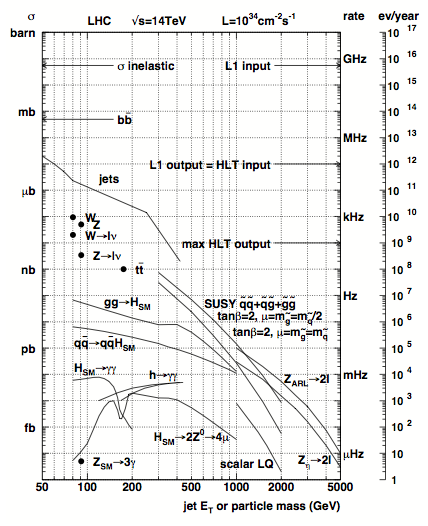
\includegraphics[width=0.49\textwidth]{Figures/detector/ppCrossSections}
  \caption{Inclusive pp cross sections (\sigma) for basic and rarer physics processes, showing some of the phenomena on the physics programme at~\ac{CMS}. Shown on the right are the interaction rates for \ac{LHC} design luminosity, \designLumi. Taken from~\cite{Cittolin:578006}.
}
  \label{fig:ppCrossSec}
  \end{center}
\end{figure}

A two tier trigger system reduces the 40~\MHz \ac{LHC} bunch crossing rate to an output of 100~\Hz, which is then saved offline to be reconstructed ready for physics analysis. 
The hardware based \ac{L1} uses fast algorithms with coarse inputs from the calorimeter and muon system to efficiently select, online (that is at the same rate as \ac{LHC} bunch crossings),
 those events that appear interesting, reducing the 40~\MHz collision rate to 100~\kHz.
A software based \ac{HLT} running on the event filter PC farm at Point 5 takes the output of the \ac{L1} trigger and reduces it further to 100~\Hz, using more sophisticated inputs and algorithms.
Performance of the subdetectors and readiness to collect data, monitored by the \ac{DAQ} system, is supervised by the trigger control system.
Events passing \ac{HLT} selection requirements are sent to the \ac{CERN} Computing Centre where complex algorithms using all the information from the \ac{CMS} detector are used to fully reconstruct the event.
More information on the~\ac{CMS} trigger can be found in Ref.~\cite{Cittolin:578006}.
%%%%%%%%%%%%%%%%%%%%%%%%%%%%%%%%%%%%%%%%%%%%%%%%%%%%%%%%%

\subsection{The L1 Trigger}
Low granularity inputs from the calorimeter and muon system are used to quickly select possibly interesting events, based on predefined and programmable algorithms and criteria.
Parts of the hardware are \ac{FPGA} based, allowing some flexibility in algorithms, while other parts are \ac{ASIC} based, with predefined criteria.
Events are selected if they show signs of interesting physics; for example have jets, electrons/photons, or muons. 
Global quantities such as total transverse energy and total missing transverse energy are also used.  
In order to see if an event contains any of these physics objects above a pre-defined energy threshold or multiplicity, 
the L1 trigger is separated into the Calorimeter Trigger, which looks for jets, photons and electrons, and the Muon Trigger, which looks for muons. 
Global quantities are computed at the \ac{GT} and combined with information from the Calorimeter and Muon triggers, 
and here a decision is made to keep or reject an event.

In the Calorimeter Trigger, information from the \ac{ECAL}, \ac{HCAL} and \ac{HF} are combined.
First, the calorimeter is split into different (geographical) regions, and electron, photon and jet finding algorithms run on the separate parts of the subdetectors at the \ac{RCT}.
Information from the different regions is then combined at the \ac{GCT}.%, where overlaps in the regions are dealt with.
In the Muon Trigger, information from the \ac{DT}, \ac{CSC} and \ac{RPC} are combined.  
Muon track finding algorithms are applied to data from the \ac{DT} and \ac{CSC} at the \ac{RMT},
and the \ac{GMT} combines information from all of the three subdetectors to get an enhanced resolution.
Inputs from the \ac{GCT} and \ac{GMT} are then combined at the \ac{GT}, 
where the decision to keep or discard an event is made.
The architecture of the L1 trigger is shown in Figure~\ref{fig:L1triggerArch}.

There is an inbuilt latency of 3.2~$\mu$s in the \ac{L1} trigger, meaning that on the first bunch crossing, it takes up to 3.2~$\mu$s to transmit the necessary information, and make a decision. 
This is driven by the data storage available for information from the tracker and preshower detectors; 
they need so much data storage that it must be saved before a L1 accept decision, and subsequent event read out, can be made.
The decisions on the rest of the bunch crossings follow at the rate of collisions, and the architecture is ready to accept another event every 25~\ns.


%picture
\begin{figure}[htbp]
  \begin{center}
  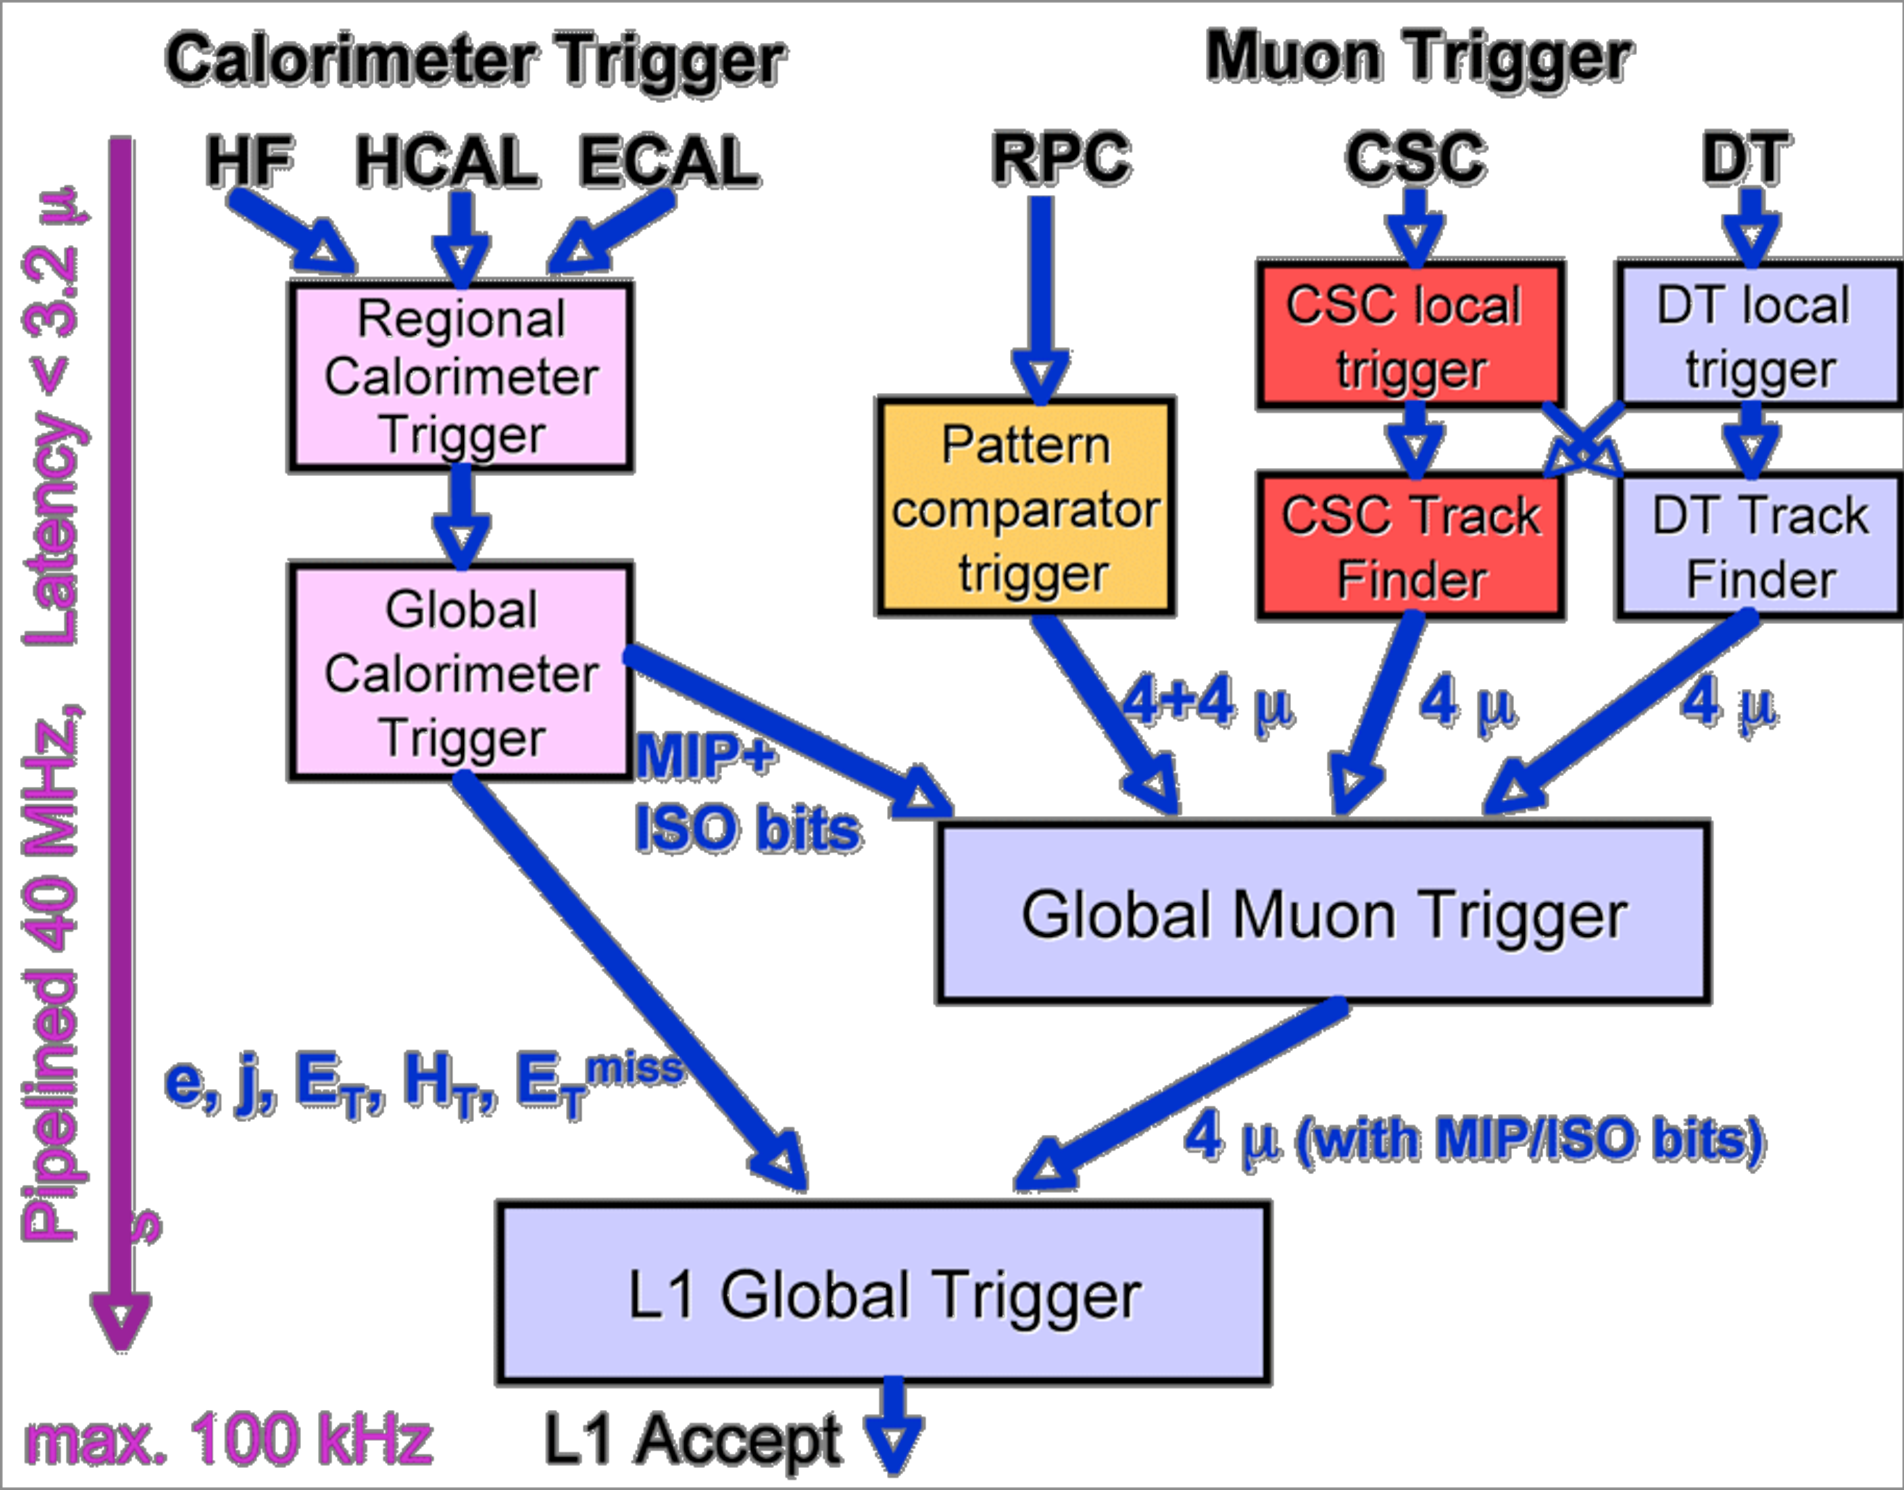
\includegraphics[width=0.6\textwidth]{Figures/detector/L1TriggerArch.pdf}
  \caption{Architecture of the \ac{L1} trigger. The calorimeter trigger takes inputs from the \ac{ECAL}, \ac{HCAL} and \ac{HF}. The muon trigger takes inputs from the \ac{DT}, \ac{CSC} and \ac{RPC}. A decision is made at the L1 \ac{GT}, using inputs from the \ac{GCT} and the \ac{GMT}, of whether to pass an event onto the \ac{HLT} or discard it.
}
  \label{fig:L1triggerArch}
  \end{center}
\end{figure}

A \ac{L1} accept decision is based upon the results of the various physics object reconstruction algorithms.
Typically, every physics analysis has a type of event it is searching for; a particular topology. 
For example, the monojet analysis looks for events with a final state of one high \pt jet and large missing transverse energy. 
At L1, it requires the global variable of an event, total missing transverse energy, above 36, 40 or 50 in \ac{L1} units of energy.
A L1 trigger menu, comprised of all of the required L1 seeds for the whole physics programme at \ac{CMS}, gives a certain bandwidth to each of the seeds. A low threshold seed will typically demand a large amount of bandwidth as more events are likely to be lower in energy, whereas a high threshold will require a lower bandwidth. 
Combined, the output to the \ac{HLT} of all of the L1 seeds in the trigger menu must not exceed the design rate of 100~\kHz.%, limited by the amount of data the \ac{HLT} can process.


\subsection{The High Level Trigger}

When an event is accepted by the L1 trigger, the full detector information for that event (consisting of around 1~MB of data) is passed onto the \ac{HLT}.
On the event filter farm, which consists of over 1000 PC's, all of the detector information for each event is processed.
Information not available at \ac{L1} becomes available. 
The additional computing power and longer time scales mean the full granularity of the calorimeter and tracker information 
(as well as \ac{L1} objects), can be used as inputs to more complex algorithms.
As a result, much more stringent requirements are used to select events of interest, creating datasets which are used for offline analysis.


An analysis will typically use more than one \ac{HLT} trigger, and similarly more than one analysis might use the same trigger (and an event pass more than one trigger).
For example, the monojet analysis %which searches for events which have one high momentum jet and large missing transverse energy,
uses a combination of three triggers which demand large missing transverse energy in every event, or a single high momentum jet in addition to large missing transverse energy.
% The monojet analysis, which searches for events which have one high momentum jet and large missing transverse energy, uses the triggers (or ``paths'')  
% \textsc{\small HLT\_MET120\_HBHENoiseCleaned}
% and
% \newline
% \textsc{\small HLT\_MonoCentralPFJet80\_PFMETnoMu95\_NHEF0p95},
% \newline
% \textsc{\small HLT\_MonoCentralPFJet80\_PFMETnoMu105\_NHEF0p95}.
% The first path requires the missing transverse energy of an event, calculated using calorimeter information only, to be greater than 120~\GeV; in addition, this is quantity is only formed from non-noisy parts of the calorimeter.
% The latter two paths are formed from events which have one jet, reconstructed using the \ac{PF} algorithm~\cite{PFT-09-001}, with transverse momentum above 80~\GeV. Additionally, the missing transverse energy, calculated also with the \ac{PF} algorithm without contributions from muons, must be above 95 or 105~\GeV, and the neutral hadronic energy fraction of the jet must be less than 0.95. 
This allows events with a monojet topology to be selected efficiently; further kinematic and topological selections are applied offline to a dataset formed of events passing these trigger requirements.
Similarly, every physics analysis uses a trigger (or triggers) suited to the topology under investigation.


In the same way that there is a L1 trigger menu, there is also a \ac{HLT} menu 
comprised of all of the \ac{HLT} trigger paths, and the bandwidths they require, which meets the needs of all of the physics analyses at \ac{CMS}.
The total bandwidth of the \ac{HLT} menu must not exceed 100~\Hz or 100 events saved offline per second, limited by the resources necessary to process and store events; namely \ac{CPU}s and disk space available.


  \chapter{Jet Algorithms for the L1 Trigger Upgrade}
\label{chap:l1jets}

In the rich hadronic environment of the \ac{LHC}, the hadronisation of quarks and gluons into jets is a major component of the physics programme of \ac{CMS}. 
Whether for standard model analyses, Higgs searches, \ac{SUSY} searches or exotic analyses,
jet reconstruction is vital for both event selection and offline analysis, for a wide range of jet kinematic requirements.
Efficient and reliable triggering on jets is therefore of key importance
and the first stage of event selection, the \ac{L1} trigger, must have an effective jet algorithm.
This is of particular significance as we look towards the \ac{LHC} upgrade, when running conditions become increasingly challenging. 
Up to double the instantaneous luminosity and centre of mass energy lead to an increase of \ac{PU} up to $\sim 70$ and far higher detector occupancies.
Jet algorithms must maintain a similar performance in this next phase of \ac{LHC} running as exhibited in the previous period of data collection.
A new L1 jet algorithm is proposed, which exploits the full granularity of the calorimeter and uses event-by-event \ac{PU} subtraction to do so. 

\section{LHC Upgrade\label{sec:LHCupgrade}}

Following the tremendously successful operation during Run I in 2010-2012, where the \ac{CMS} and \ac{ATLAS}
experiments collected around 5~\fbinv at 7~\TeV and 20~\fbinv at 8~\TeV,
the \ac{LHC} is currently in a period of shut-down, termed ``Long Shutdown 1'' (LS1). 
Magnet interconnections are being replaced and the dipole magnets are undergoing a quench training programme. 
These improvements to the \ac{LHC} magnets will allow safe acceleration of protons up to 7~\TeV in each beam, and sustained operation at $\sqrt{s}=13~\TeV$, eventually to achieve the design energy of 14~\TeV.
This will nearly double the available centre-of-mass energy as compared to Run I, potentially making Run II a discovery run - opening up more phase space and therefore opportunities for finding new physics.
Instantaneous luminosity will also increase, with the aim of providing the statistics required to search for the rarest processes, as well as shed more light on the properties of the boson discovered during Run 1~\cite{Aad:2012tfa,Chatrchyan:2012ufa,HiggsEvidence}. 
After a period of a year or so of running after LS1 termed ``Run II'', the \ac{LHC} will again undergo a period of shutdown, 
``Long Shutdown 2'' (LS2), in which improvements to the accelerator injector chain will be made - with the aim of providing much greater instantaneous luminosities. 
The potential luminosity performance of two scenarios for future running of the \ac{LHC} is shown in Table~\ref{lumiProgramme}. 

\begin{table}[h]
\begin{tabular}{c|c|c|c|c}
Scenario & \# bunches & $\mathcal{L}$ (cm$^{-2}$s$^{-1}$) & Pile-up & L ($\fbinv$/year) \\ \hline
25~ns & 2760 & 9.2 $\times 10^{33}$ & 21 & 24 \\ 
50~ns & 1260 & 2.2 $\times 10^{34}$ & 40-76 & 45 \\ \hline
\end{tabular}
\caption{\label{lumiProgramme} Two of the possible luminosity performances for \ac{LHC} running during Run II, taken from ~\cite{Tapper:1556311}.}
\end{table}


If the machine operates at 50~\ns, the instantaneous luminosity will double compared to that of Run I, with PU expected to more than double from around 20 inelastic collisions per bunch crossing to in excess of 70.
%As a result, the number of interactions per second will also increase; and detector occupancies and trigger rates will soar.
Not only will the number of interactions per second increase due to the higher instantaneous luminosity, but the increased centre of mass energy means the energy of these interactions will also increase. 
Consequently, for a particular trigger (say, for example a single jet trigger), many, many more events will pass a particular energy threshold as compared to Run I. 
As a result, the trigger rate will soar.

For a single jet trigger, where the jet (reconstructed offline) is required to be above 128~\GeV, 95\% of jets which have been matched to this offline jet and reconstructed using the existing \ac{L1} jet algorithm are above 150~\GeV - where the higher \ac{L1} threshold is due to poorer \ac{L1} reconstruction than offline reconstruction. 
In a typical run during 2012 (PU=15, $\mathcal{L}=0.4 \times 10^{34}$~cm$^{-2}$s$^{-1}$), a \ac{L1} jet threshold of 150~\GeV corresponds to a rate of 1.1~\kHz.
In the high \ac{PU} runs during 2012, this trigger rate rose to 3.6~\kHz (PU=45, $\mathcal{L}=1.1 \times 10^{34}$cm$^{-2}$s$^{-1}$); and simulation shows that in similar conditions but at 14~\TeV, a trigger rate of 14~\kHz is expected.
The total rate of all of the \ac{L1} triggers is capped to 100~\kHz by restrictions from the \ac{HLT}, 
and a balanced trigger menu is desirable to satisfy all of the physics demands of \ac{CMS}.
Therefore, individual trigger rates must be kept reasonably low to ensure the total \ac{L1} trigger rate is acceptable.  
The only way to maintain low trigger rates in the more challenging run conditions is to increase energy thresholds.
Figure~\ref{tab:L1TrigMenuCurrentSystem} shows an illustrative \ac{L1} trigger menu for the upgraded \ac{LHC}, for bunch spacings of 25 and 50~\ns. 
Thresholds have had to be significantly raised to maintain a total rate below 100~\kHz; for example, the single jet threshold is increased to 170~\GeV and 205~\GeV for 50 and 25~\ns bunch crossings respectively.


\begin{figure}[htbp]
  \begin{center}
  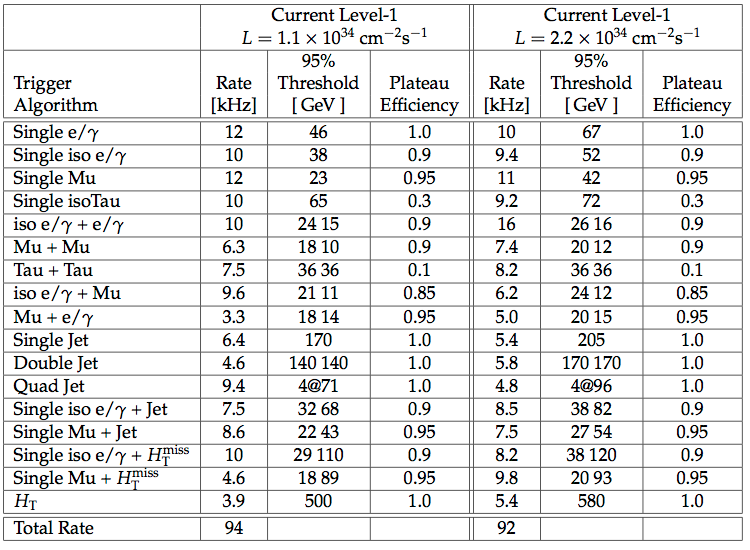
\includegraphics[width=0.95\textwidth]{Figures/l1jets/triggerThresholdCurrentL1Table.png}
  \caption{The projected \ac{L1} trigger menu using the current \ac{L1} system and algorithms, at 14~\TeV, for illustration purposes. In the left hand column, all of the different triggers contributing to the menu are shown. In the centre (right-hand) columns, the projected L1 trigger rate, 95\% threshold and plateau efficiency are shown for running conditions with bunch spacing of 50~\ns, $\mathcal{L}=1.1 \times 10^{34}$~cm$^{-2}$s$^{-1}$, PU=50 (25~ns, $\mathcal{L}=2.2 \times 10^{34}$~cm$^{-2}$s$^{-1}$, PU=50), taken from~\cite{Tapper:1556311}.
}
  \label{tab:L1TrigMenuCurrentSystem}
  \end{center}
\end{figure}


For the physics requirements of \ac{CMS} the necessary increase in \ac{L1} thresholds, and corresponding increase in offline (analysis) thresholds, is an unacceptable compromise as lower energy final states are crucial to many analyses and keeping as much physics, at as low thresholds as possible, is desirable.
To cope with the challenges of the \ac{LHC} upgrades, and to enable new, better performing algorithms to be developed so the physics performance of Run I can be maintained, or bettered, the \ac{CMS} \ac{L1} trigger is also undergoing upgrades. 



\section{CMS Trigger Upgrade}
Upgrades to the electronics of the calorimeter trigger, muon trigger and global trigger are under way in order 
to meet the triggering demands of \ac{CMS}.
These upgrades involve installing additional interconnections between the systems, reducing the current huge diversity of electronics cards to a small number of multi-purpose and adaptable cards, using high bandwidth optical links and modern, high powered \ac{FPGA} processing chips. 
These upgrades not only allow more information from the detector subsystems to be used as inputs to improved (more complex) algorithms, due to increased logic resources and fast links, 
but crucially also allow far more flexibility in the \ac{L1} trigger system. 
In Run I, the ability to adapt the trigger algorithms and menu to evolving \ac{LHC} run conditions proved vital in reducing trigger rates and improving efficiencies. 
Increasing the flexibility by making more of the system adaptable, and more of the cards standardised, will only improve the trigger and enhance its longevity. 
Having the ability to easily update software and firmware, as well as trigger architecture, in response to unforeseen circumstances - not just in the planned \ac{LHC} upgrades to 2016 but far beyond - will put \ac{CMS} in an excellent position for data collection.

The new \ac{L1} trigger is being installed during LS1, and will be commissioned and run concurrently with the existing trigger during Run II. 
Once it's performance has been tested and verified, the upgraded system will be available after LS2, at which point the existing system will no longer be operable.
Here, I discuss in detail the calorimeter trigger upgrade, as this is what the proposed jet algorithm, detailed in this chapter, relies upon.
More information on the muon trigger and global trigger upgrade can be found in~\cite{Tapper:1556311}.



\subsection{Calorimeter Trigger Upgrade}
The calorimeter trigger uses information from the \ac{ECAL} and \ac{HCAL} to look for electrons/photons and jets, as described in the previous chapter.
It currently is based upon a traditional trigger design; where the detector is spatially segmented into different processing nodes, each of which deals with the data from each geographical region, and does so at every bunch crossing.
The desire for far more flexibility in triggering motivates a new approach to the upgrade trigger architecture, known as time-multiplexing.
Instead of splitting the detector into geographical regions and sending the data to different processors at every bunch crossing, 
a \ac{TMT} places all of the data from the detector in a single processor across several bunch crossings.
No data is thrown away at any stage of the process, and all of the data, at its full granularity, is available in the same card making many more algorithms possible.


\subsubsection{Traditional Trigger Architecture}
A conventional trigger architecture is shown in Figure~\ref{fig:tradTrig}.
The calorimeter is split into geographical regions in $\eta-\phi$, 
and at every bunch crossing data from the individual regions are sent to different processors.
Boundaries between these regions must be duplicated in each implicated processor, to ensure that any objects found along the boundary are sufficiently dealt with.
To achieve a compact implementation, at each stage of the trigger process the volume of data is reduced and the minimal information with which to make a decision is passed onto the \ac{GT}. 
Therefore, a lot of the information from an event is discarded before a decision at the \ac{GT} is made.
In addition, the current calorimeter trigger does not use the full granularity of information available, and the combined \ac{ASIC} and \ac{FPGA} hardware, although permitting some flexibility in algorithms and parameters, is restricted by a fixed data flow. 
Not all algorithms can therefore be implemented, and the coarse inputs limit the possible performance.

\begin{figure}[h!]
%\vspace{-1.cm}
\begin{center}
  \includegraphics[scale=0.78]{Figures/l1jets/TraditionalTrigger.png}
\caption{Conventional trigger architecture, showing data processing in regions. Taken from~\cite{RoseTrig}.}
\label{fig:tradTrig}
\end{center}
\end{figure}

Energy clusters are built into physics objects with which the \ac{GT} can make a decision over two processing layers. 
Trigger towers, consisting of groups of $5 \times 5$ crystals in the \ac{ECAL}, and the corresponding blocks of the \ac{HCAL}, are themselves grouped into $4 \times 4$ arrays or ``regions''. 
These regions are used as inputs to the various object algorithms.
In the first layer, the `Regional stages' in Figure~\ref{fig:tradTrig}, the regions, or clusters of transverse energy are assigned a type; electron/photon-like, if energy is predominantly in the \ac{ECAL}, otherwise hadron-like.
In the second processing layer, the `Global Stages', the cluster type is identified as an electron/photon or tau (for high energy or isolated deposits respectively), and non-isolated clusters are grouped together to form jets.
The jet finding algorithm looks for energy deposits in windows of $3 \times 3$ regions, with the requirement that the central region has a larger transverse energy deposit. 
The top four candidates are passed onto the global trigger, with the rest discarded.
Also in this layer of processing, the value and direction of total missing transverse energy are calculated from the sum of energy deposits across the calorimeter, 
and jet candidates above threshold are summed to give the total hadronic energy content, known as $H_{\mathrm{T}}$.    




\subsubsection{Time Multiplexed Trigger}
A time-multiplexed trigger architecture is shown in Figure~\ref{fig:TMTrig}. 
In a similar way as the \ac{HLT}, it will consist of parallel nodes, each of which process individual events concurrently.
All of the data from an event - from the whole $\eta - \phi$ range of the calorimeter and at full granularity - are sent to an individual processor. 
The first processor receives the data from the first bunch crossing over $N$ clock cycles (where the length of a clock cycle is equal to the time between bunch crossings, 25 or 50~\ns).
The data from the second bunch crossing are sent to the second processor, again over $N$ clock cycles, and so on; where there are more than $N$ processors in total, as each processor needs time to process each event.
After the first processor has processed all of the data from the first bunch crossing and passed it on to the next stage of the trigger, the `Demux' in Figure~\ref{fig:TMTrig} (some $N+X$ clock cycles after the first bunch crossing where $X$ is the time taken to process and send on the data), it can then receive data from another bunch crossing.
Developments in large \ac{FPGA} chips and increased rate and volume of data transmission in optical fibres make this kind of architecture possible for the upgraded CMS calorimeter L1 trigger, whereas it was not when the current trigger was designed and built. 
The system latency, $N+X$, is now small enough, due to the increased processing power and bandwidths, that it is viable in hardware for the huge amounts of data and short time-scale that the trigger demands~\cite{TMT_dem}. 

\begin{figure}[h]
%\vspace{-1.cm}
\begin{center}
  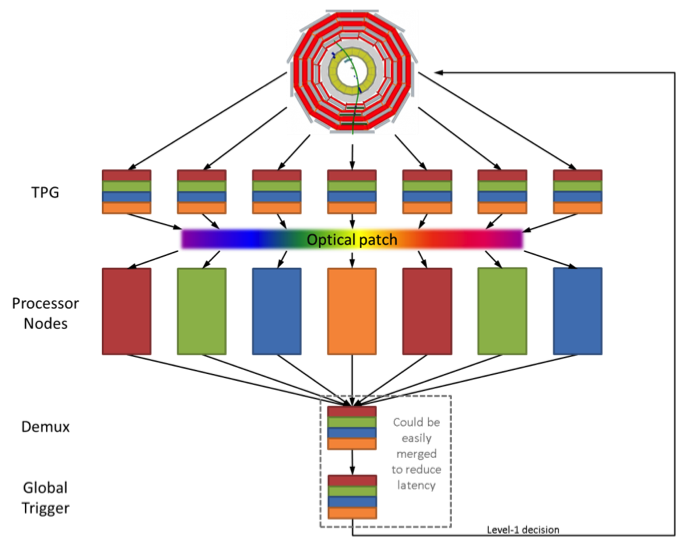
\includegraphics[scale=0.8]{Figures/l1jets/TMTrigger.png}

\caption{Time-multiplexed trigger architecture, showing data pipelining to different processing nodes. Taken from~\cite{RoseTrig}.}
\label{fig:TMTrig}
\end{center}
\end{figure}


With all of the data, at full granularity, in one single processor, many more algorithms for object reconstruction are possible. 
Tower level calorimeter inputs (rather than region level inputs) will be available, increasing the granularity by a factor 4$^{2}$, with similarly improved spatial resolutions.
There is also scope for an array of additional variables, using information from the whole calorimeter. For example, the average energy deposit for each row in $|\eta|$ or ring of $\phi$ can be calculated, and used to give an estimate of \ac{PU} on an event-by-event basis.
In the remainder of this chapter, a jet algorithm is proposed for the upgraded \ac{L1} calorimeter trigger.
More detail on the CMS \ac{L1} calorimeter trigger upgrade can be found in Ref.~\cite{1748-0221-9-01-C01006}.


%%%%%%%%%%%%%%%%%%%%%%%%%%%%%%%%%%%%%%%%%%%%%%%%%%%%%%%%%%%%%%%%%%%%%%%%%%%%%%%%%%%%%%%%%%%%%%%
%        _ ______ _______            _      _____  ____  _____  _____ _______ _    _ __  __ 
%       | |  ____|__   __|     /\   | |    / ____|/ __ \|  __ \|_   _|__   __| |  | |  \/  |
%       | | |__     | |       /  \  | |   | |  __| |  | | |__) | | |    | |  | |__| | \  / |
%   _   | |  __|    | |      / /\ \ | |   | | |_ | |  | |  _  /  | |    | |  |  __  | |\/| |
%  | |__| | |____   | |     / ____ \| |___| |__| | |__| | | \ \ _| |_   | |  | |  | | |  | |
%   \____/|______|  |_|    /_/    \_\______\_____|\____/|_|  \_\_____|  |_|  |_|  |_|_|  |_|
%        
%%%%%%%%%%%%%%%%%%%%%%%%%%%%%%%%%%%%%%%%%%%%%%%%%%%%%%%%%%%%%%%%%%%%%%%%%%%%%%%%%%%%%%%%%%%%%%%

\section{Algorithm for jet reconstruction at L1}
\label{Sec:Algo}
A jet algorithm to reconstruct, filter and calibrate \ac{L1} jets is proposed, for the upgraded \ac{CMS} calorimeter trigger.
It is assumed that all of the \ac{L1} calorimetric information for a single event is available at 
the same time in the same place; that is, all of the information from a single bunch crossing being in one single processing chip.
This is compatible with the \ac{TMT} architecture which will be available after LS2 at \ac{CMS}. 

Using tower level information, the algorithm creates a tunable sized jet at each site on the calorimeter, filters out zero-energy jets and repeats, to get the `best' 13 jet candidates per event. The average jet energy density for each event is calculated, and subtracted from the energy deposited across the calorimeter in order to perform \ac{PU} subtraction on an event-by-event basis. 
The 13 jet candidates are then calibrated to offline energy. 
This algorithm is compared to the current L1 jet algorithm.% and the `best' possible algorithm, which is taken to be the \ac{PF} algorithm with towers used as inputs.
A much improved spatial resolution is seen, as well as enhanced, and crucially, more \ac{PU} independent energy resolution. 
The resulting trigger turn-on curves for various jet energy thresholds, and trigger rates for single and multijet triggers are improved compared to the current algorithm, as well as the global variable \HT.
This jet algorithm was the proposed jet algorithm in the \ac{CMS} \ac{L1} trigger Technical Design Review, Ref.~\cite{Tapper:1556311}.


\subsection{Jet Reconstruction}

The proposed jet algorithm uses the full granularity of the calorimeters available at \ac{L1}; that is, $5 \times 5$ \ac{ECAL} crystals grouped together into towers, with the corresponding block of \ac{HCAL}. 
In the centre of \ac{CMS}, each tower measures $0.087\times0.087$ in the $\eta-\phi$ plane, with the $\eta$ dimension increasing as $\eta$ increases; see Figure~\ref{fig:towerGeo}. 
In total there are 72 towers in the $\phi$ direction, and for $|\eta|\leq3.0$ (the barrel region), 56 towers in the $\eta$ direction.
The sum of energy deposits in both the \ac{ECAL} and \ac{HCAL} at each tower is used as input to the algorithm. 

\begin{figure}[ht]
%\vspace{-1.cm}
\begin{center}
  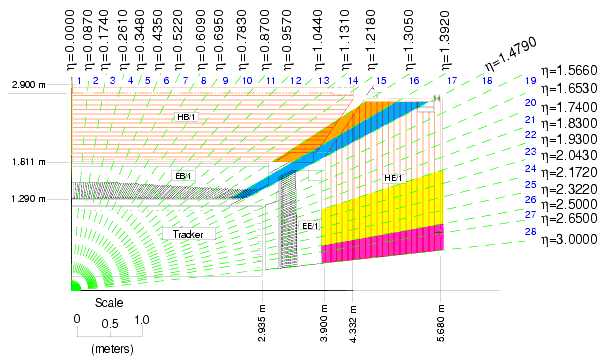
\includegraphics[scale=0.67]{Figures/l1jets/towerGeometry}

\caption{Layout of trigger towers in the $r-z$ projection, for $0<\eta<3.0$. Both \ac{ECAL} and \ac{HCAL} towers are shown.}
\label{fig:towerGeo}
\end{center}
\end{figure}

A group of $n \times n$ towers is combined to form a jet candidate, where the energy of that jet candidate is the sum of the $n \times n$ towers it consists of. 
The jet size, $n$, is completely flexible, as well as the jet shape. 
Jet sizes of $8\times8$ to $12\times12$ were studied, and both circular and square jets. 
This compares with the current \ac{L1} jet algorithm, which consists of equivalent $12\times12$ square jets 
- where the towers are incorporated into regions, each measuring $4\times4$ towers; see Figure~\ref{fig:jetcartoon} for a comparison of the current and proposed upgrade jet geometry.
For circular jets the size $n$ represents the length of the diameter, 
for square jets it represents the length of the side. 

\begin{figure}[ht]
%\vspace{-1.cm}
\begin{center}
  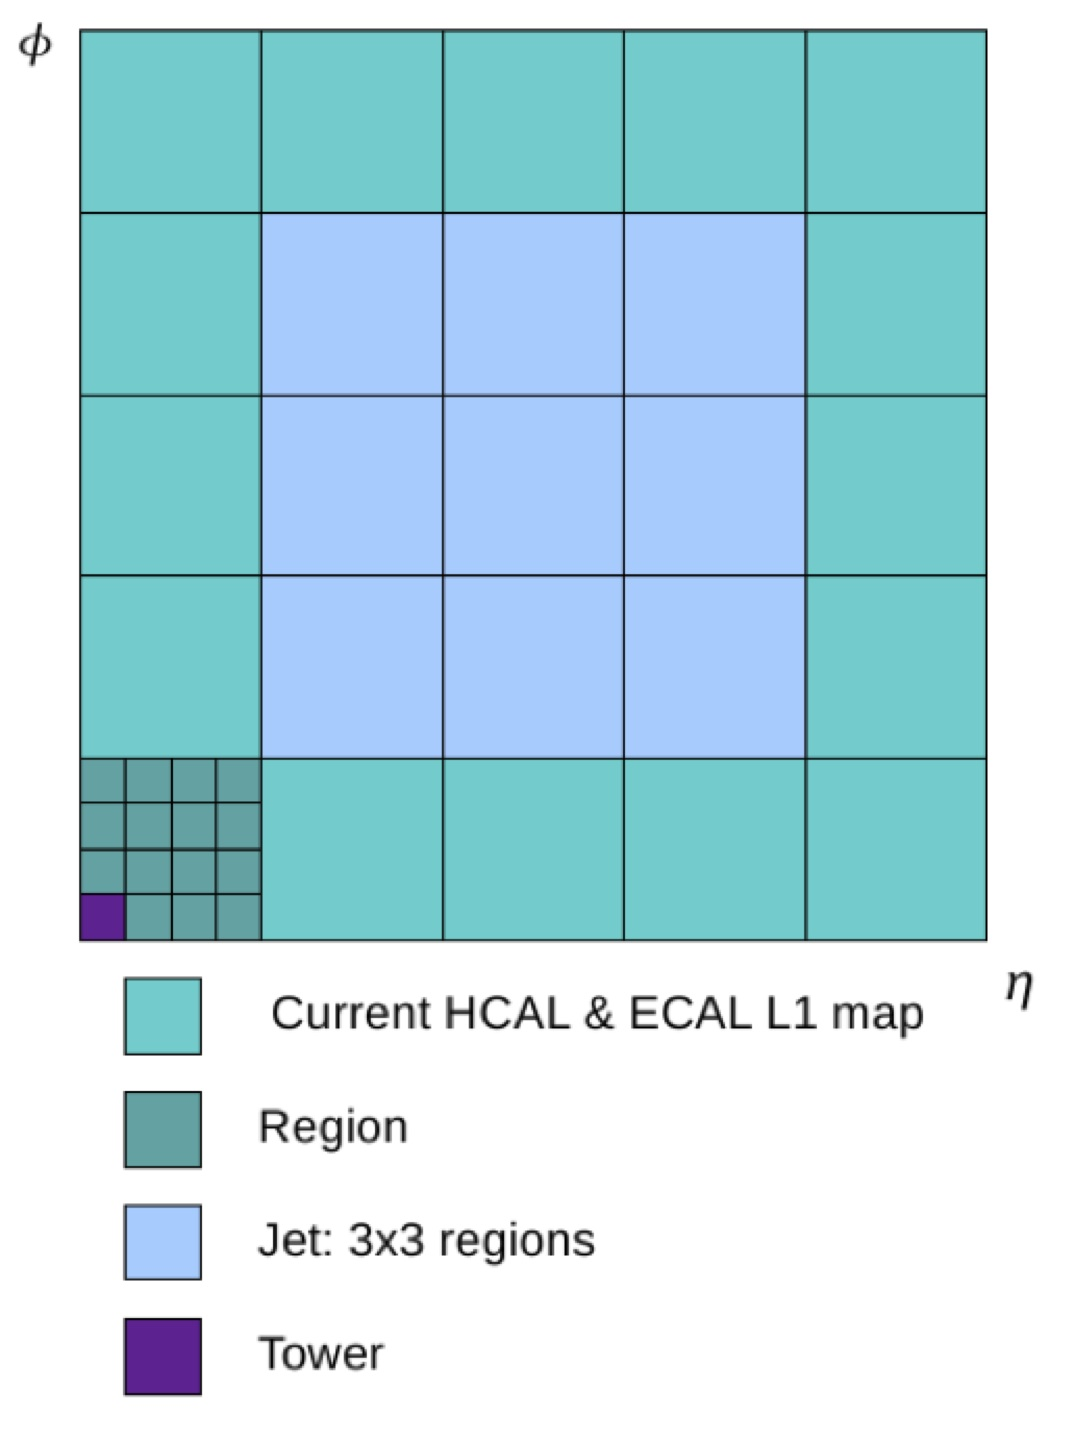
\includegraphics[scale=0.34]{Figures/l1jets/CurrentL1Jet.jpg}
  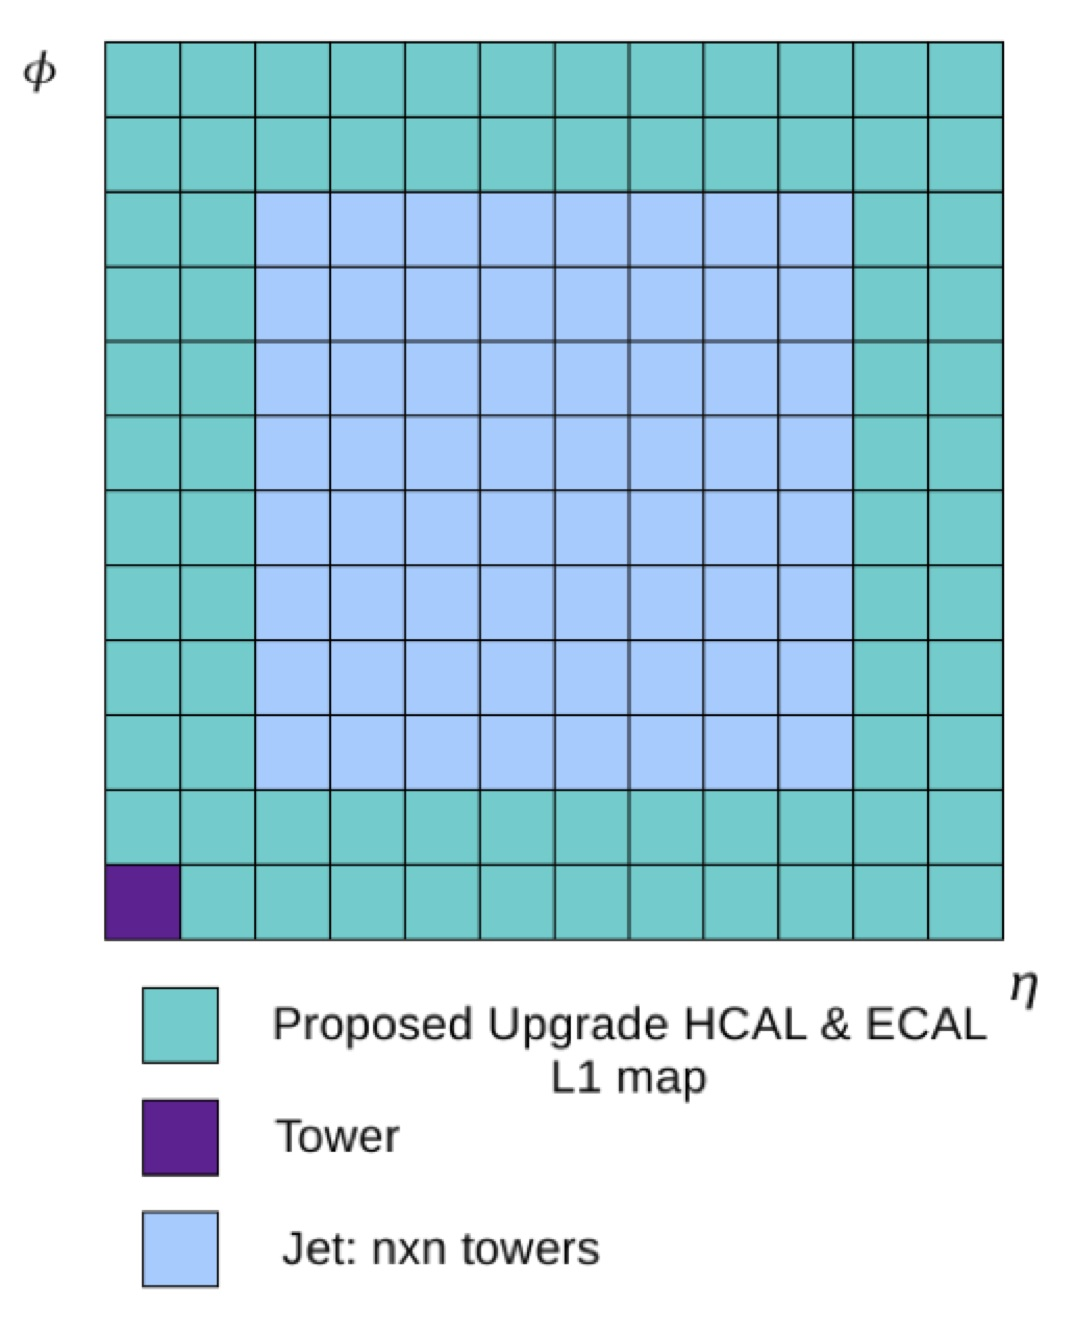
\includegraphics[scale=0.37]{Figures/l1jets/UpgradeJet.jpg} 
\caption{Comparison of the current \ac{L1} jet map, left, with the proposed upgrade jet map, showing a $8\times8$ square jet, right.}
\label{fig:jetcartoon}
\end{center}
\end{figure}


A candidate is created at each individual tower, using a ``sliding window'' approach. 
Only jet candidates with non-zero energies are passed onto the next stage, 
however there remains a huge jet multiplicity at this first stage of jet creation. 
There is a jet for every non-zero tower, and a huge number of overlapping jets as each tower contributes to $n^{2}$ different jets, or, equivalently, each jet candidate has $(2n - 1)^{2}$ overlapping jets.
Figure~\ref{slide} shows some of jet candidates which overlap, shown in red, with a single jet candidate measuring $4\times4$ towers and square in shape, shown in purple.
The window of all overlapping candidates is shown in blue; and measures $10\times10$ towers.
The resulting numerous overlapping jets must be sorted and filtered to find the highest energy jet of the candidates.

\begin{figure}[ht!]
%\vspace{-1.cm}
\begin{center}
%  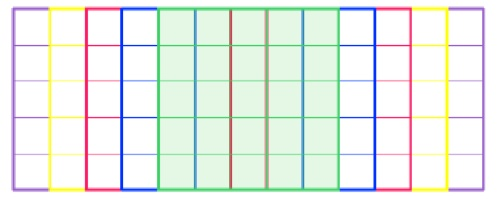
\includegraphics[scale=0.37]{Figures/l1jets/JetOverlaps.jpg}
  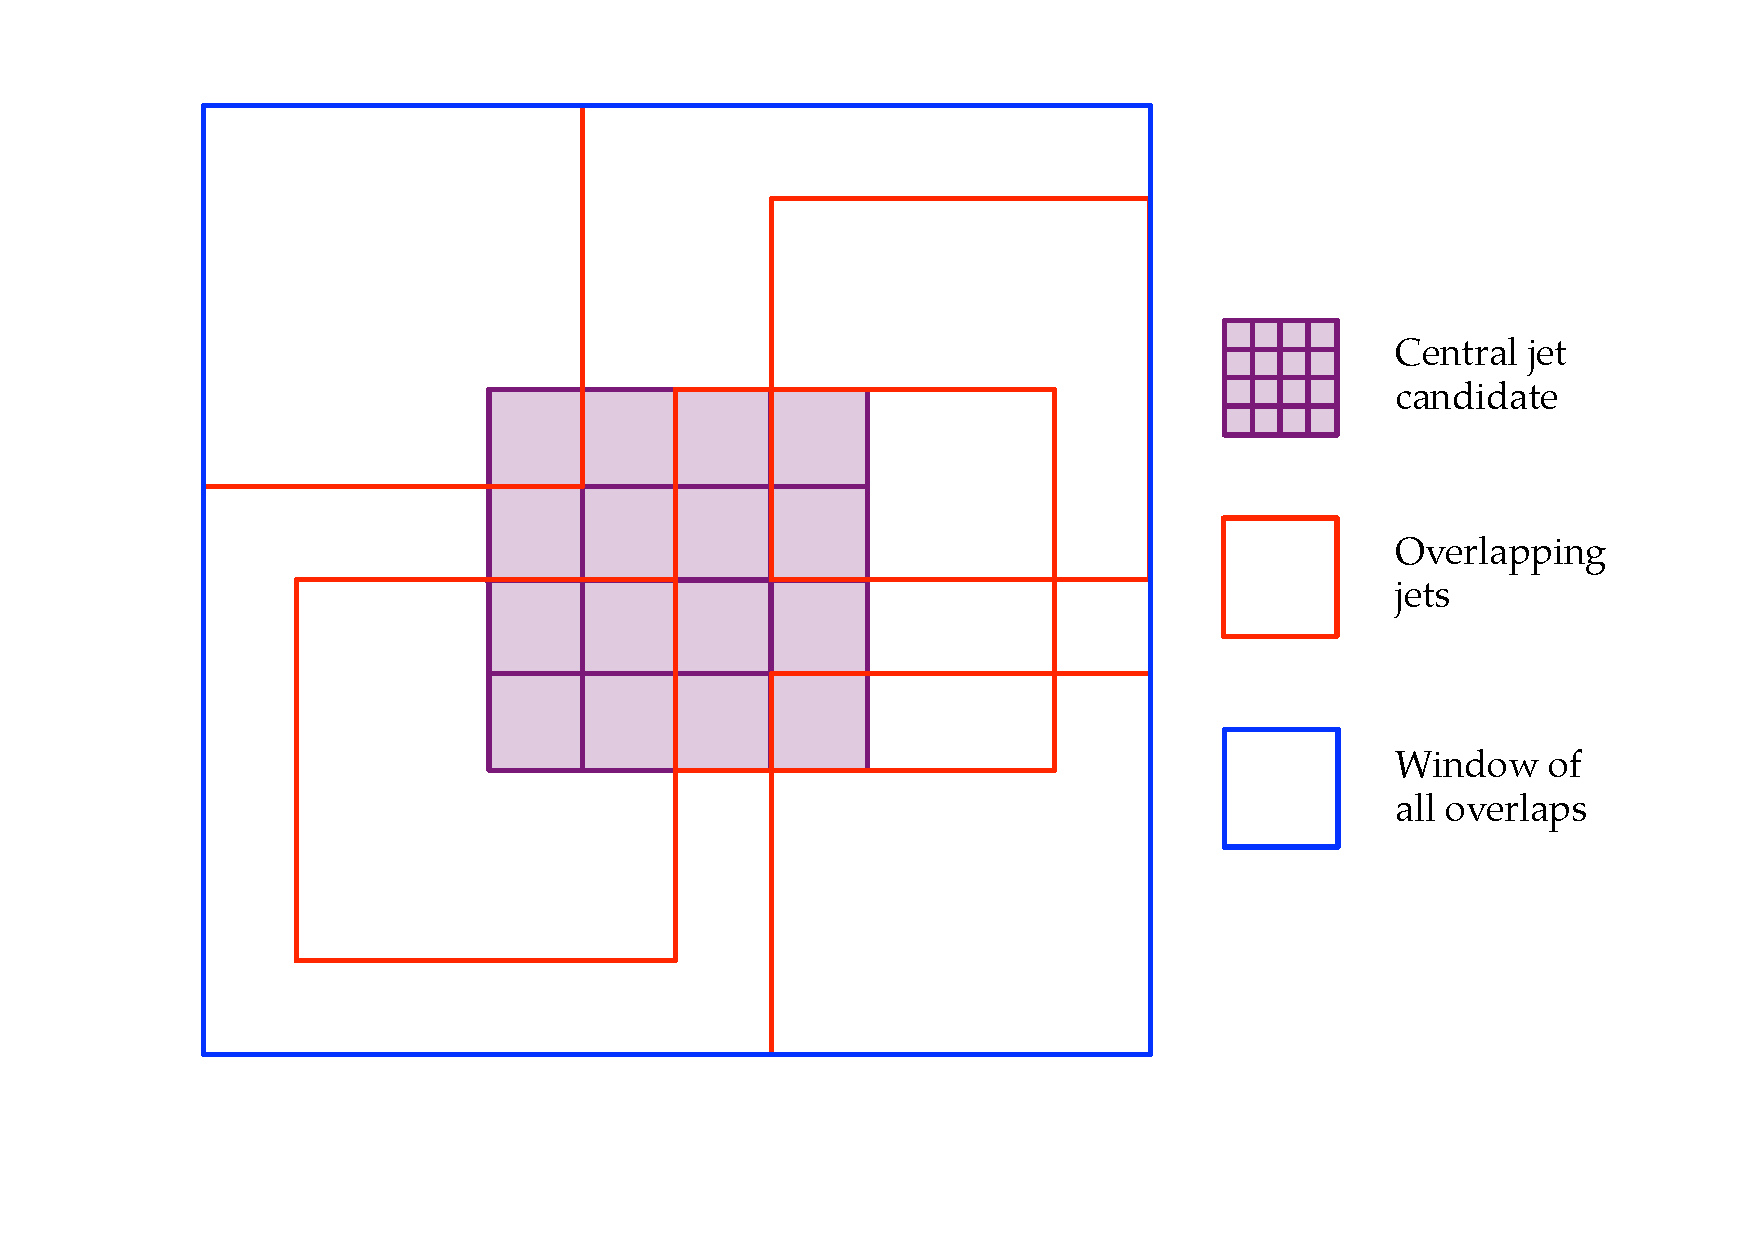
\includegraphics[scale=0.37]{Figures/l1jets/jetoverlaps}
\caption{A few of the overlapping jets of one $4\times4$ jet (centre, purple), are shown in red. The window of all of the jet overlaps is shown in blue, measuring $10\times10$. These overlapping jets must be sorted and filtered to keep only the most energetic jet.}
\label{slide}
\end{center}
\end{figure}

To give the best angular resolution, the $\eta$ and $\phi$ coordinates of the jets are energy weighted,
\begin{eqnarray}
\eta_{jet} &=& \frac{\sum{\eta_{\rm tower} \cdot E_{\rm tower}} } {\sum{ E_{\rm tower} } }  \\
\phi_{jet} &=& \frac{\sum{\phi_{\rm tower} \cdot E_{\rm tower}} } {\sum{ E_{\rm tower} } } . 
\end{eqnarray}
Here, the sum is over all of the towers in a jet window and $\eta_{\rm tower}$, $\phi_{\rm tower}$ are the coordinates of the individual towers within a jet, $E_{\rm tower}$ is the transverse energy deposit in the tower and $\eta_{jet}, \phi_{jet}$ are the coordinates of the jet.


In previous studies diameter 8 circular jets gave the best angular resolution, so these are presented here. 
\textcolor{red}{Remake plots and include here}



\subsection{Jet Filtering} 
The jet collection must be sorted and filtered to remove the numerous overlaps.
Firstly, all jets in each event are ordered in energy using a bitonic sort.
This is a recursive parallel sorting algorithm suitable for implementation in hardware.
It takes $2^N$ inputs and sorts in $N$ steps using a series of bitonic sequences and splits.

However, there is often more than one overlapping jet of a particular energy. 
An asymmetry parameter in $\eta$ and $\phi$ is also considered for each jet when this is the case:
\begin{equation}
 \begin{split}
 A_{\eta, \phi} = & \sum \left( \text{Constituent tower energies in positive } \eta , \phi \right) \\ & - \sum \left( \text{Constituent tower energies in negative } \eta, \phi \right) 
 \end{split}
\label{eqn:Asym}
\end{equation}
A jet with all of its energy in the central tower will have $A_{\eta, \phi} = 0$ 
whereas a jet of the same energy with all energy deposits in an outer tower
 will have large $|A_{\eta, \phi}|$. 
If overlapping jets have the same energy, they are instead sorted 
to give the lowest asymmetry parameter.
The first element in the sorted list is then the most energetic jet, with its energy concentrated most centrally within the $n\times n$ window.

 The sorted list is then filtered to remove jets which overlap with with this first jet.
 The process is repeated until 13 separate jets are found. 
 This number is somewhat arbitrary, and is limited by hardware at some high number.
 
Jets are sorted initially in one dimension, along $\eta$ or $\phi$, and overlaps in one dimension are removed. 
The resulting list of the most energetic jets along or around the calorimeter is then sorted in the other direction to give the final jet collection.


\subsection{Event-by-event estimation of pile-up} 

The measurement of the PU contribution to the jet energy 
is evaluated event by event using a method inspired by the paper of 
Cacciari and Salam~\cite{rho_jetarea} and already used to correct offline jets.
In a pp collision with a large number of overlapping proton-proton interactions, 
a large number of relatively soft jets originate from PU and are distributed roughly 
evenly across the calorimeter.  
The median jet transverse energy is therefore very likely to come from PU, and gives a good estimate of the typical transverse energy of a \ac{PU} jet in the event.
Further, the energy density of the median jet transverse energy gives a good estimation of the energy density due to \ac{PU} across the calorimeter.
The energy released by \ac{PU} per unit area in each event, denoted by $\rho$, can therefore be estimated using the median jet transverse energy, and the area of the jet:
\begin{eqnarray}
 \rho^{\rm L1} &=& \frac{ \langle E^{\text{L1 jet}}_{\rm T} \rangle }{A_{\text{L1 jet}}}
\end{eqnarray}
where $\langle E^{\text{L1 jet}}_{\rm T} \rangle$ denotes the median jet transverse energy, and $A_{\text{L1 jet}}$ denotes the jet area.
The energy of all jets in an event can then be corrected for the energy density due to \ac{PU} by
simply subtracting from all jets in an event using
\begin{eqnarray}
 \text{PU corrected }E_{T} &=& E_{T} - \rho^{\rm L1} \times A_{\text{L1 jet}} ,
 \label{eqn:PUsub}
\end{eqnarray}
because the energy density due to \ac{PU} across the calorimeter is assumed to be uniform. 
This assumption is valid for \ac{PU} values of order $\sim50$, however as \ac{PU} increases above 100 pp collisions in each bunch crossing, simulation shows many more soft \ac{PU} jets are expected to lie in the forward regions of the detector, so an $\eta$ dependent \ac{PU} subtraction may be more suitable for very high \ac{PU} scenarios.
This is not investigated here, but is within the capabilities of the upgraded trigger system.

In the following we show the effect of PU subtraction in the measurement of the
jet energy. The same quantity could also be used to correct contribution of \ac{PU} to quantities used to defined electrons/photons; isolation parameters, and the ratio of transverse energy deposits in the \ac{HCAL} and \ac{ECAL}.


\subsection{Calibration to the jet energy scale \label{jet_calib}}
The raw jet energies from the calorimeter towers must be corrected to the jet energy scale. 
Different regions of the calorimeter give different responses so a set of calibration constants 
in \pt and $\eta$ are derived. %: so-called "L2L3 corrections".
A non linear regression method is used on an independent subsection of 
20,000 events collected using single muon trigger; that is, events which contain a least one muon, 
which often implies hadronic activity in the opposite hemisphere to the muon and so the data sample provides a sufficient number of jets to do a statistically meaningful calibration. 

Once the \ac{L1} upgrade jets have been created, sorted and filtered, the value of the average energy density due to \ac{PU}, $\rho^{\rm L1}$, 
is calibrated to the jet energy scale by comparing it with $\rho$ calculated offline for each event.
The corrected \ac{PU} subtraction parameter is applied to the \ac{L1} jets in the event according to Equation~\ref{eqn:PUsub}, in order that they 
can be calibrated to the offline jets which have been similarly \ac{PU} subtracted.
The leading offline jet in each event, where the jet is formed using the anti-k$_{\rm T}$ algorithm with radius parameter of 0.5 and inputs from the calorimeter alone, ``AK5 Calo jets'', is matched to a L1 jet within a cone of 
$\Delta R = \sqrt{ (\eta_{L1} - \eta_{offline})^2 + (\phi_{L1} - \phi_{offline})^2} < 0.5$.
The use of AK5 Calo jets gives reconstructed offline jets as close as possible to those created at \ac{L1}, as both are built using calorimeter information alone.
The values of \pt and $\eta$ for the matched \ac{L1} and offline jets are used as inputs to a multi-variant analysis.  
This provides a lookup table of multiplication factors binned in values of the L1 jet $\eta$ and $\pt$. 
Applying this calibration to the \ac{L1} jets gives a calibration independent of PU. 

The distribution of L1 jet \pt, where each jet has been matched to an offline jet, before and after the calibration has been applied is shown in Figure~\ref{prepostCalib}. 
Momenta are much more closely matched after the calibration has been applied.

\begin{figure}[t!]
\begin{center}
  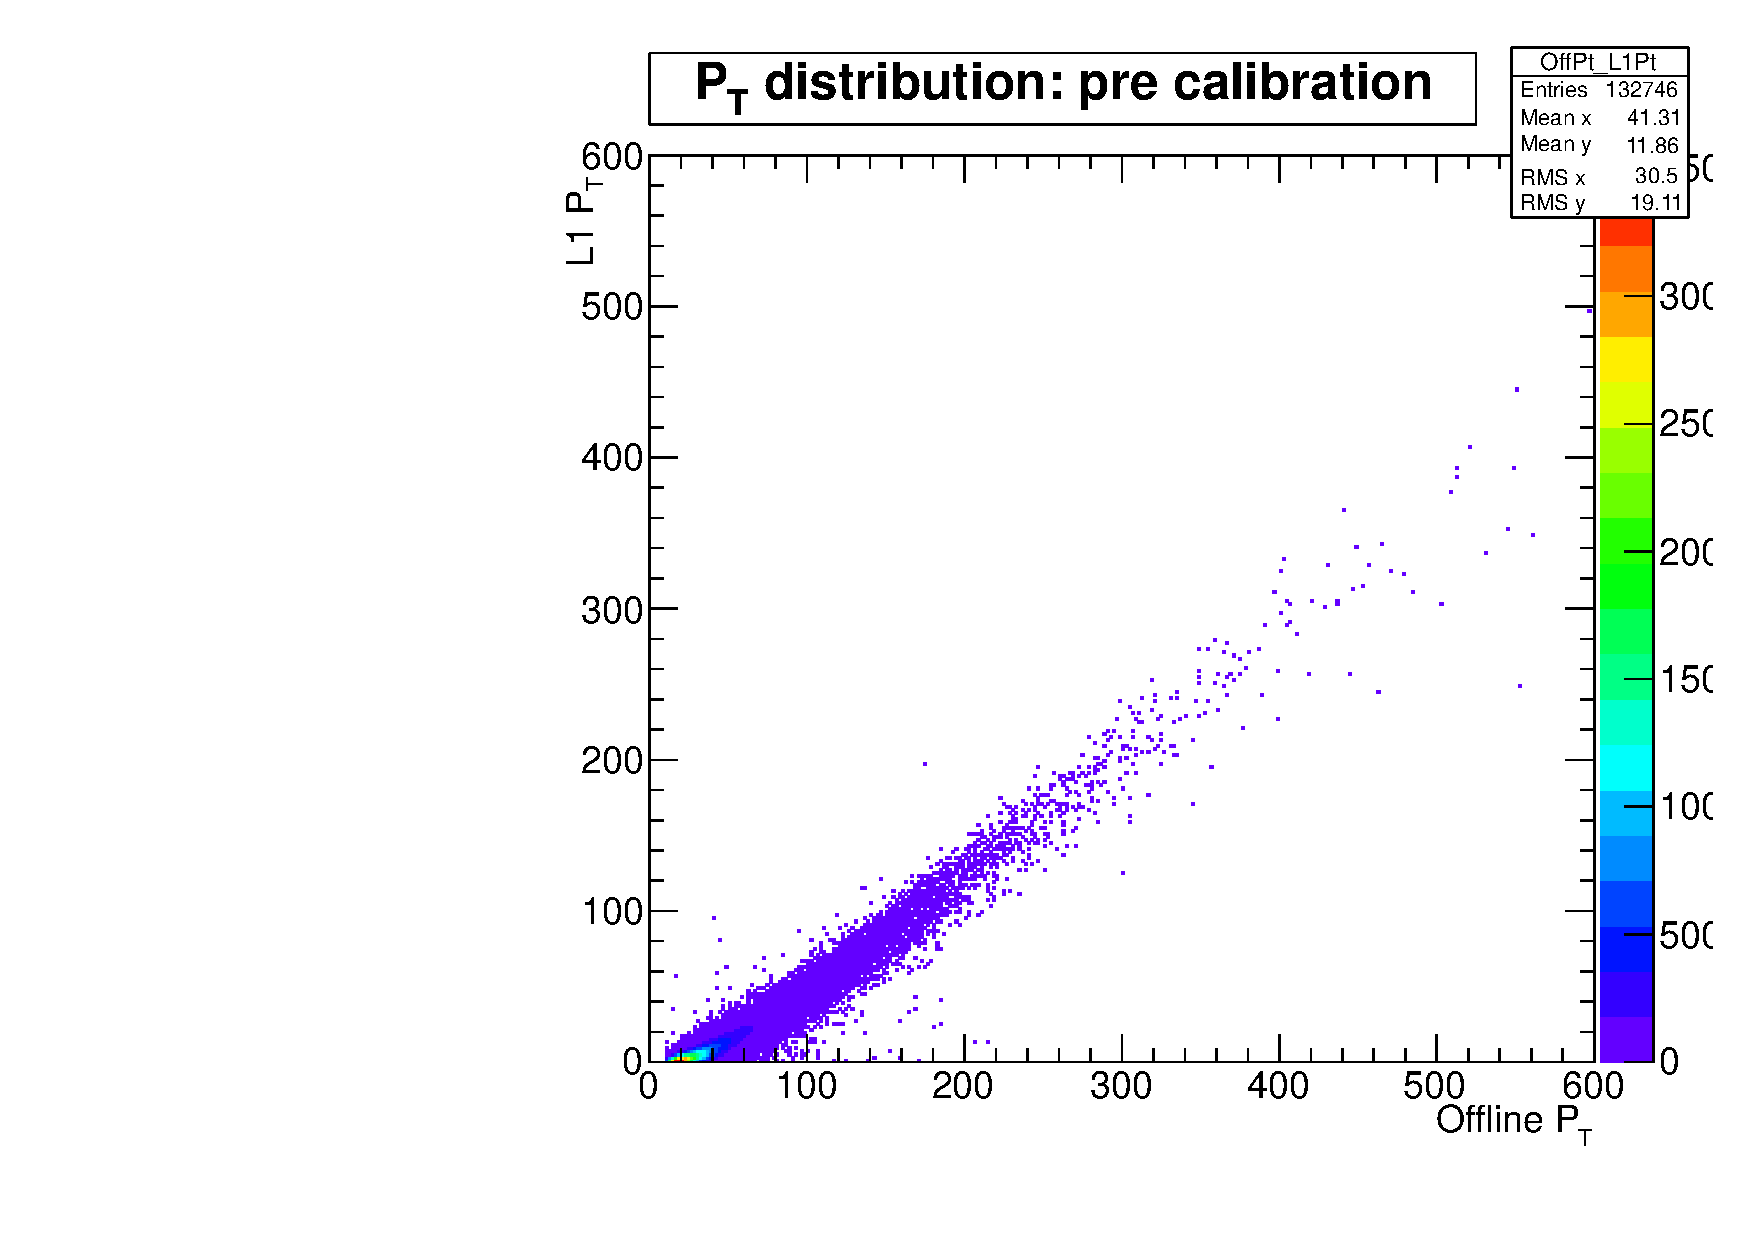
\includegraphics[scale=0.32]{Figures/l1jets/PreCalib.pdf}
  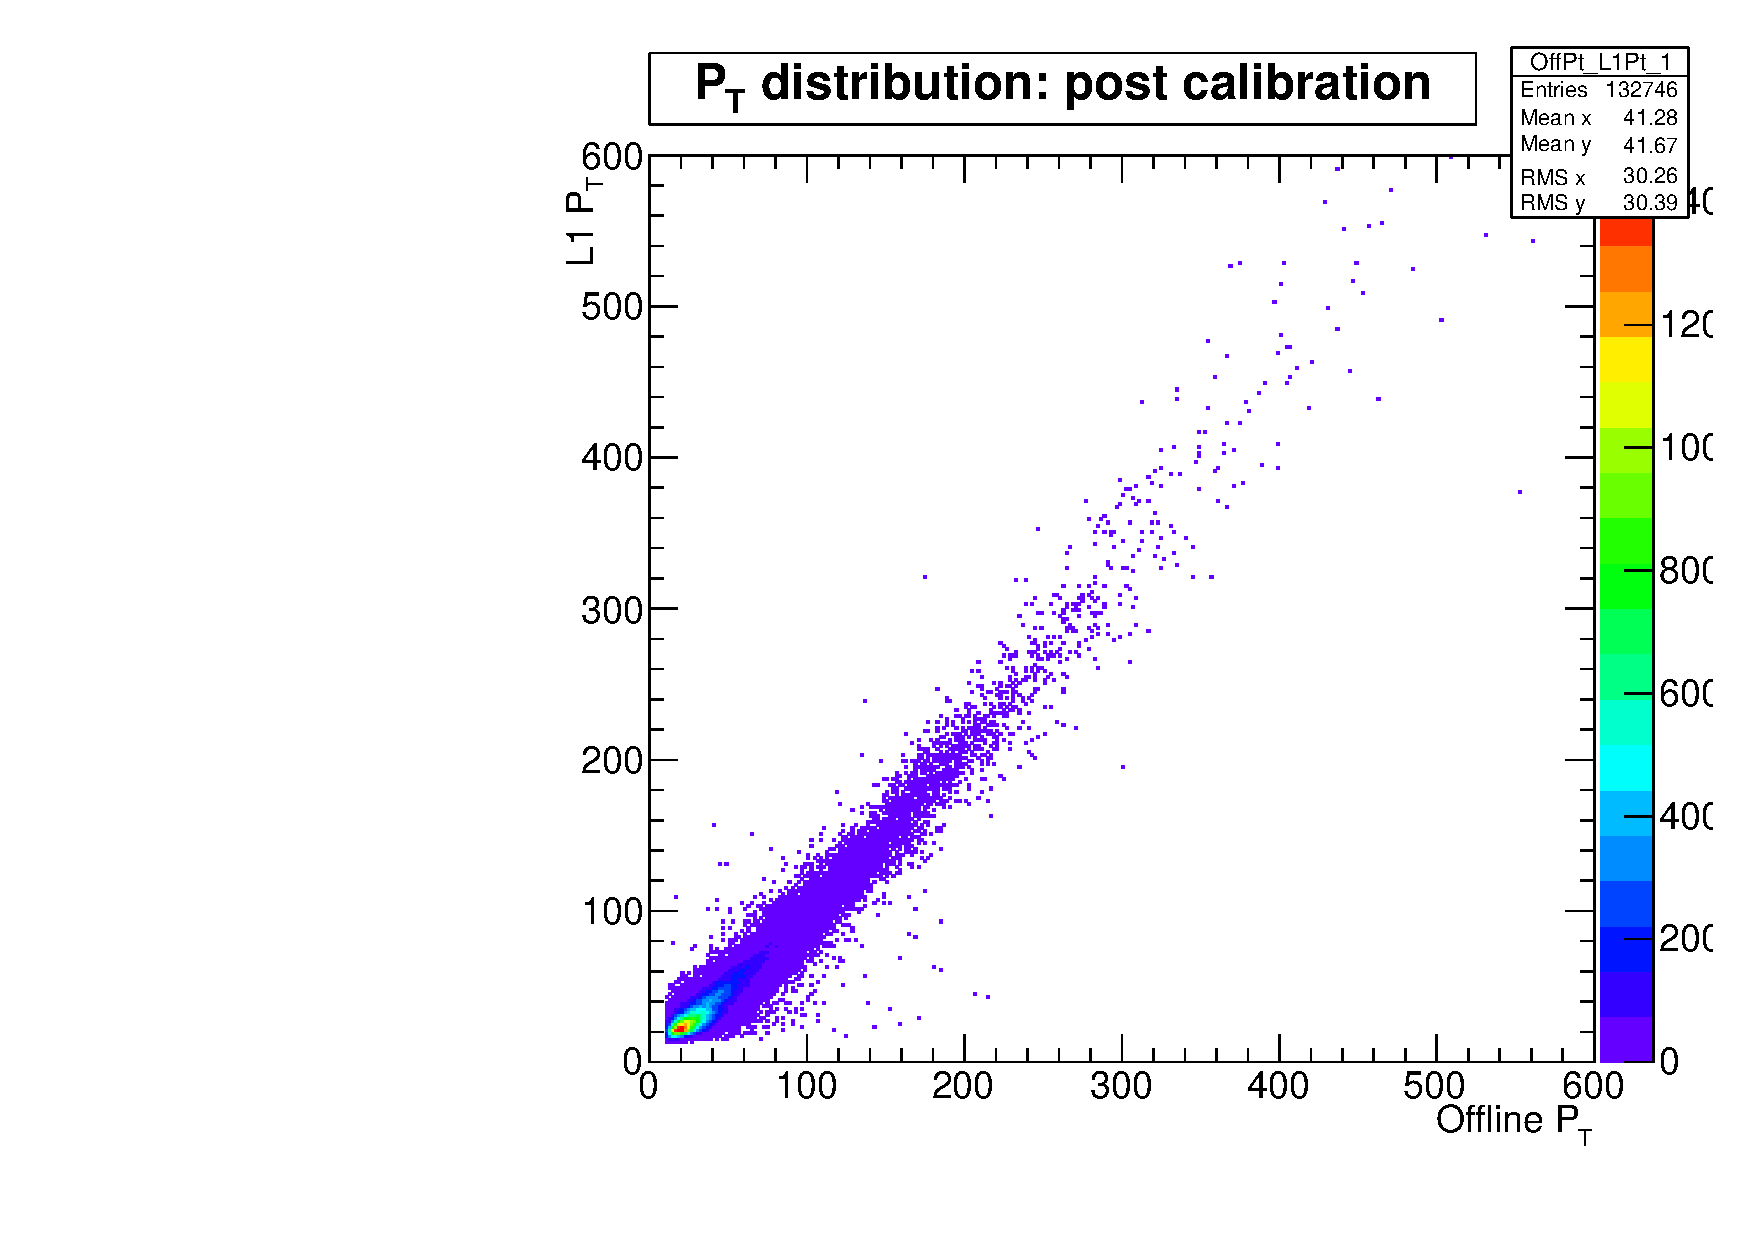
\includegraphics[scale=0.32]{Figures/l1jets/PostCalib.pdf}
\caption{The \pt distribution of \ac{L1} jets that have been matched, within a cone of $\Delta R<0.5$, to offline jets reconstructed with the anti-k$_{\rm T}$ algorithm using a radius parameter of 0.5 and calorimeter information as input only. The distribution shown before a \pt and $\eta$ calibration has been applied is shown on the left, and after the calibration has been applied on the right. In both distributions, \ac{PU} has been subtracted from both jet collections. }
\label{prepostCalib}
\end{center}
\end{figure}



\section{Upgrade L1 Jet Algorithm Performance}
Jet performance can be characterised by angular and energy resolutions, efficiency of reconstruction and trigger rates. The proposed upgrade \ac{L1} jets were simulated using data that was collected in high \ac{PU} conditions during 2012, where no triggers were applied. The \ac{LHC} run used for the study had an average of 45 primary vertices per bunch crossing.  

\subsection{Angular and Energy Resolutions}

Resolutions are measured as compared to offline AK5 Calo jets, as described in Section~\ref{jet_calib}. 
The leading offline jet (which must have $\pt > 20$~\GeV) is matched to a L1 jet within $\Delta R < 0.5$, and the resolutions are defined as:
\begin{eqnarray}
\sigma_{\eta} &=& \eta_{offline} - \eta_{L1} \\
\sigma_{\phi} &=& \phi_{offline} - \phi_{L1}\\
\sigma_{\pt} &=& \frac{ \pt^{L1} - \pt^{offline} } { \pt^{offline} } 
%\Delta_{\rho} &=& \frac{\rho_{AK5Calo} - \rho_{L1} } {\rho_{AK5Calo}}
\end{eqnarray}  

Angular and energy resolutions of the proposed upgrade algorithm compared to the current system are shown in Figure \ref{JetRes}.
There is a much improved angular resolution as the upgrade jets take advantage of the full granularity of the calorimeter. In high PU data, the energy resolution is improved due to the PU subtraction. 
With the current \ac{L1} jet algorithm, there are a significant number events in which the leading offline jet has been matched to low energy PU L1 jets, giving a negative value of $\sigma_{\pt}$ and giving rise to the significant negative tail in the distribution.

\begin{figure}[t!]
\begin{center}
  \includegraphics[scale=0.32]{Figures/l1jets//etaRes.pdf}
    \includegraphics[scale=0.32]{Figures/l1jets//phiRes.pdf}
       \includegraphics[scale=0.32]{Figures/l1jets//ptRes.pdf} 
\caption{Resolution of $\eta$, $\phi$ and \pt for high \ac{PU} data taken by the \ac{CMS} detector in 2012. There is a clear improvement with the upgrade jets, plotted in blue, in both angular resolutions and energy resolution.}
\label{JetRes}
\end{center}
\end{figure}

Crucially, the energy resolution of the upgrade jet algorithm shows a much reduced dependence on \ac{PU}, shown in Figure~\ref{JetResPU}.
This is evidence that the event-by-event \ac{PU} subtraction has the intended effect, 
reducing the worsening effect of additional primary vertices on the jet energy resolution, 
and the upgrade jet algorithm is therefore is expected to show a reduction in rates as compared to the current algorithm.

\begin{figure}[t!]
\begin{center}
  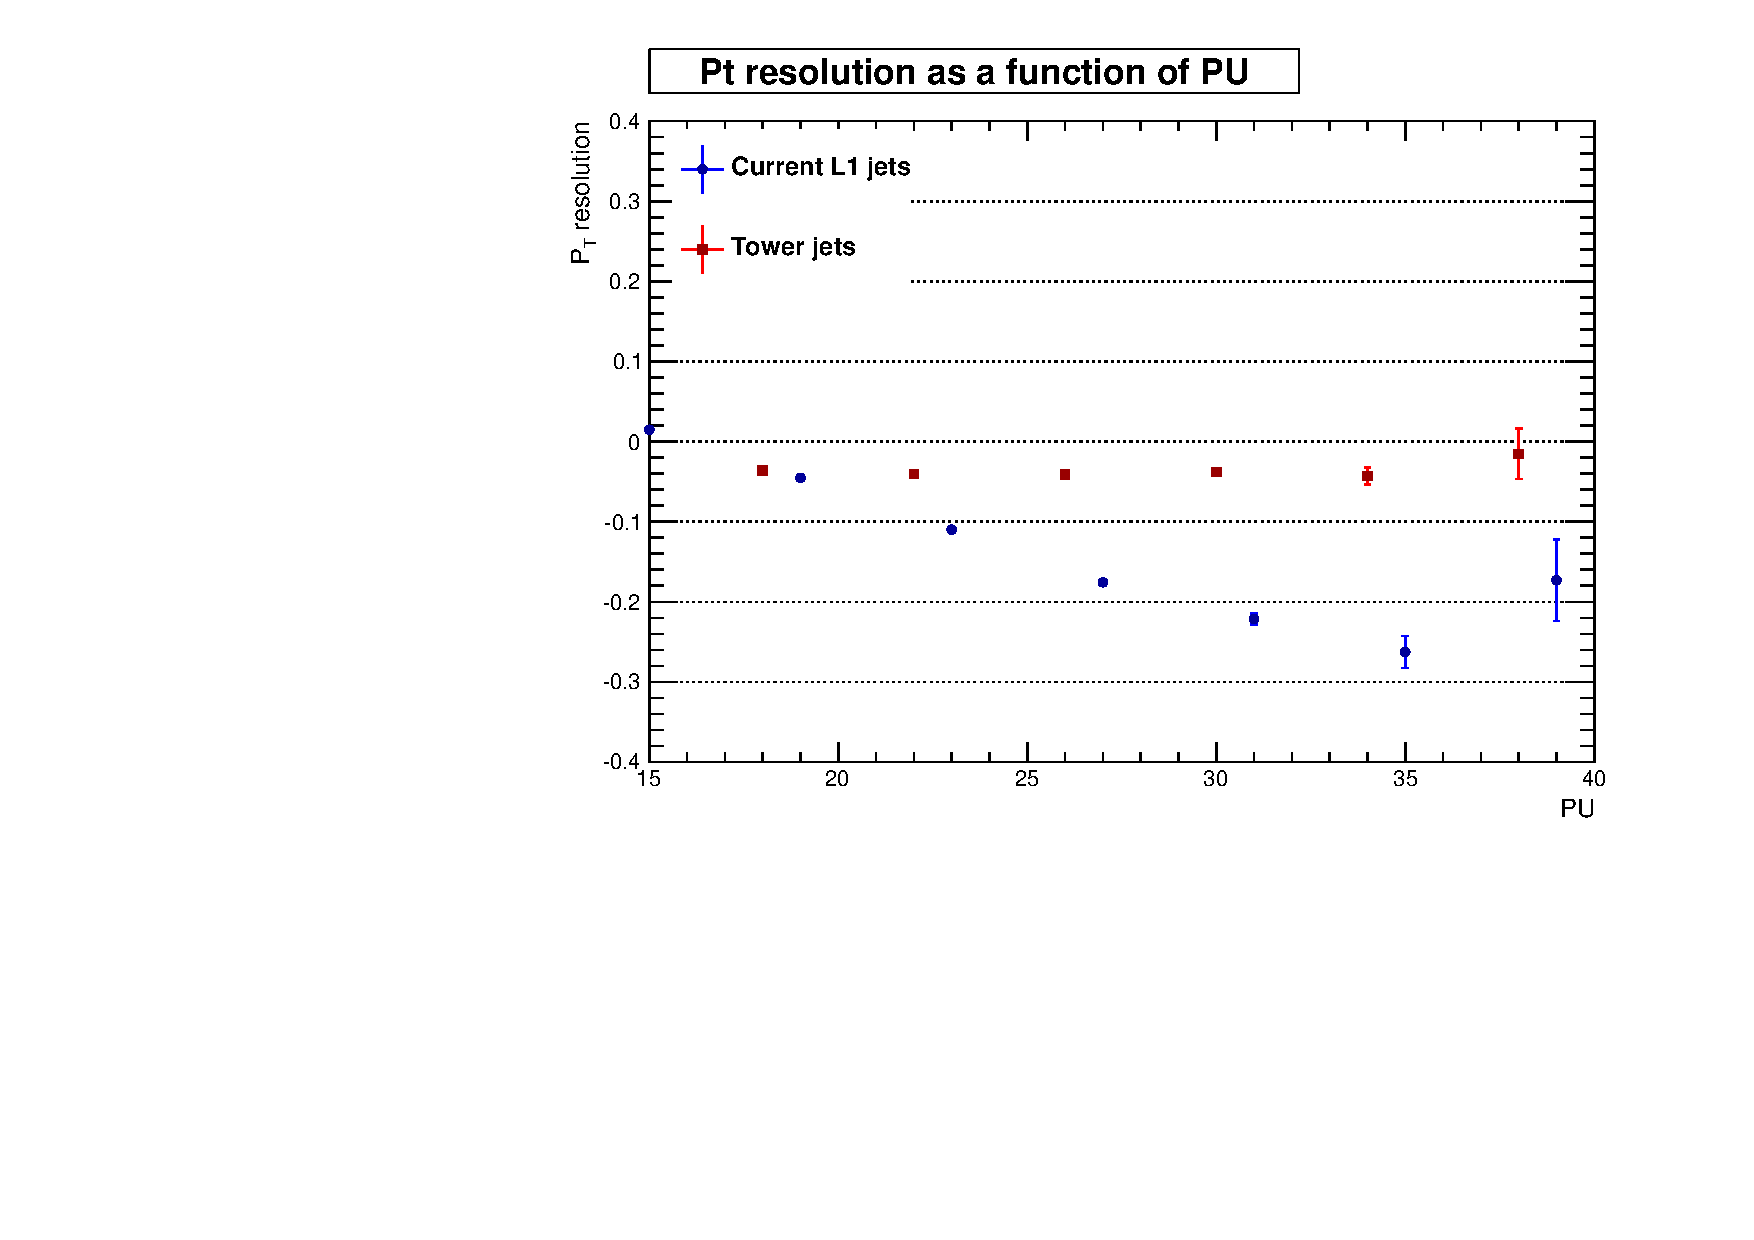
\includegraphics[scale=0.52]{Figures/l1jets/Ptres_vsPU.pdf}
\caption{The \ac{PU} dependency of the \ac{L1} jet energy resolution for both the current algorithm and the upgrade algorithm, where the resolution is taken as the RMS of the PU distribution shown in Figure~\ref{JetRes}, for different \ac{PU} bins. There is a clear improvement with the upgrade jets, plotted in blue, which shows independence of \ac{PU} up to \ac{PU}$\sim$40.}
\label{JetResPU}
\end{center}
\end{figure}

\subsection{Trigger efficiencies}
The trigger efficiencies for various L1 jet transverse energy thresholds are measured, as compared to AK5 Calo jets, to show the effectiveness of the proposed algorithm at reconstructing jets which have been measured offline, which are treated as the ``truth''.
If the leading \ac{L1} jet in each event above a certain energy threshold is matched to an offline jet, the energy of the matched offline jet is plotted. 
All matched offline jet energies are also plotted. 
By taking the ratio between these two distributions we attain trigger turn on curves, shown in Figures~\ref{JetTO_lowPU} and \ref{JetTO_highPU}.

The sharpness of the turn on curve is due to the energy resolution of the jet algorithm.
If all of the \ac{L1} jets have reconstructed energies that exactly equal the energies of the offline jets to which they are matched,
i.e. $\sigma_{\pt} = 0$, there would be a delta function at the value of the jet energy threshold of the trigger.
The turn on would be instant at the specified trigger threshold.
%
The plateau efficiency of the turn on is dictated by the matching efficiency of the jet algorithm.
If all \ac{L1} jets are perfectly matched to offline jets then the algorithm is fully efficient at reconstructing jets at \ac{L1} and the plateau efficiency is 1.

The turn on curves shown in Figure~\ref{JetTO_lowPU} are taken from data taken using the same single muon trigger as was used for jet calibration, where the presence of at least one muon in each event implies there is often hadronic activity in the opposite hemisphere of the detector to the muon. 
This is a relatively low \ac{PU} set of events, with approximately 20 p-p interactions per bunch crossing. 
Figure~\ref{JetTO_highPU} shows the performance at \ac{PU} of approximately 45, a data sample which has lower statistics.
The sizeable negative tail shown in the momentum resolution for the current algorithm in Figure~\ref{JetRes} is 
evident in the bump at low momentum in the left hand plot.
Events in which relatively soft jets due to \ac{PU} have been reconstructed above threshold at \ac{L1} are 
matched to very soft \ac{PU} jets reconstructed offline and cause the behaviour at low \pt.
Because the soft \ac{PU} jets have effectively been removed from the upgrade \ac{L1} jet collection, this is not the case for the upgrade trigger turn ons.


\begin{figure}[t!]
\begin{center}
  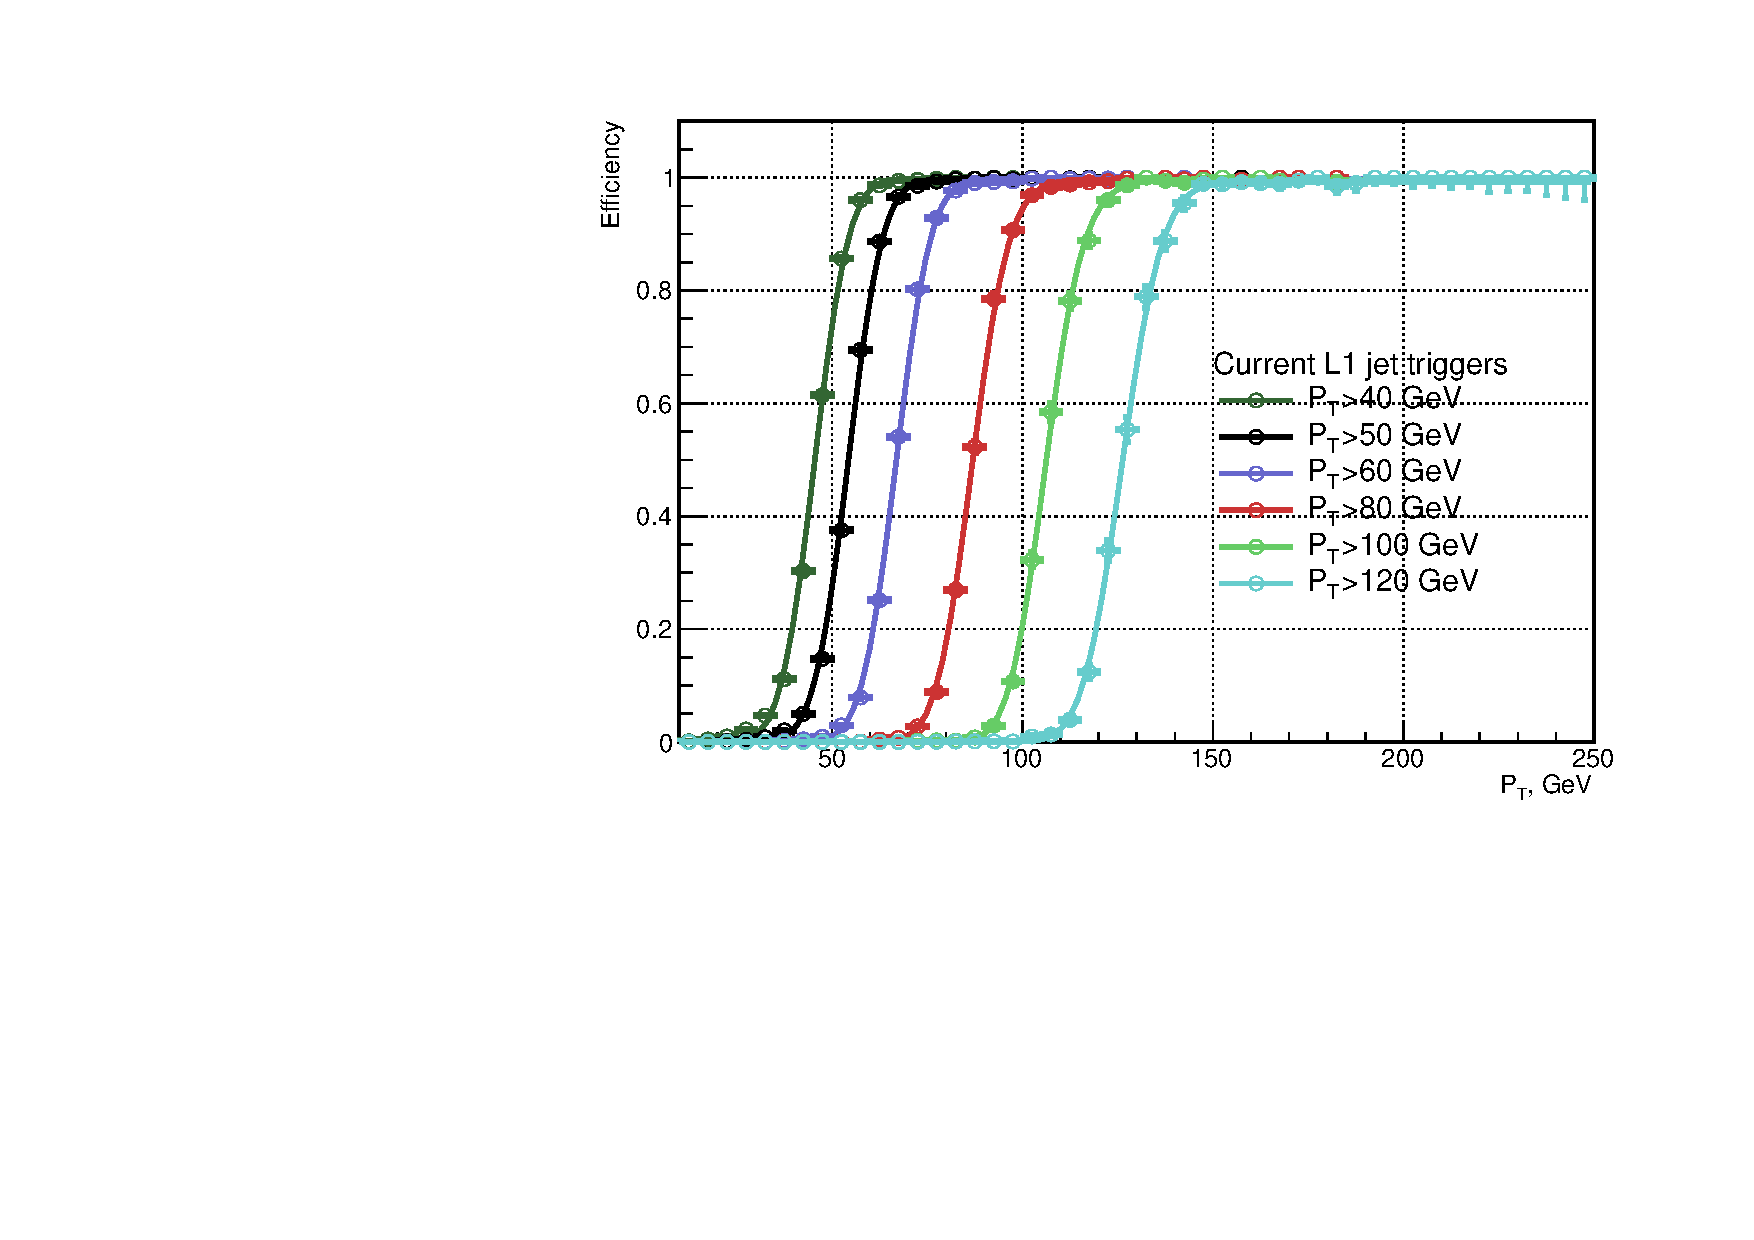
\includegraphics[scale=0.37]{Figures/l1jets//CurrentL1JetTriggers.pdf}
    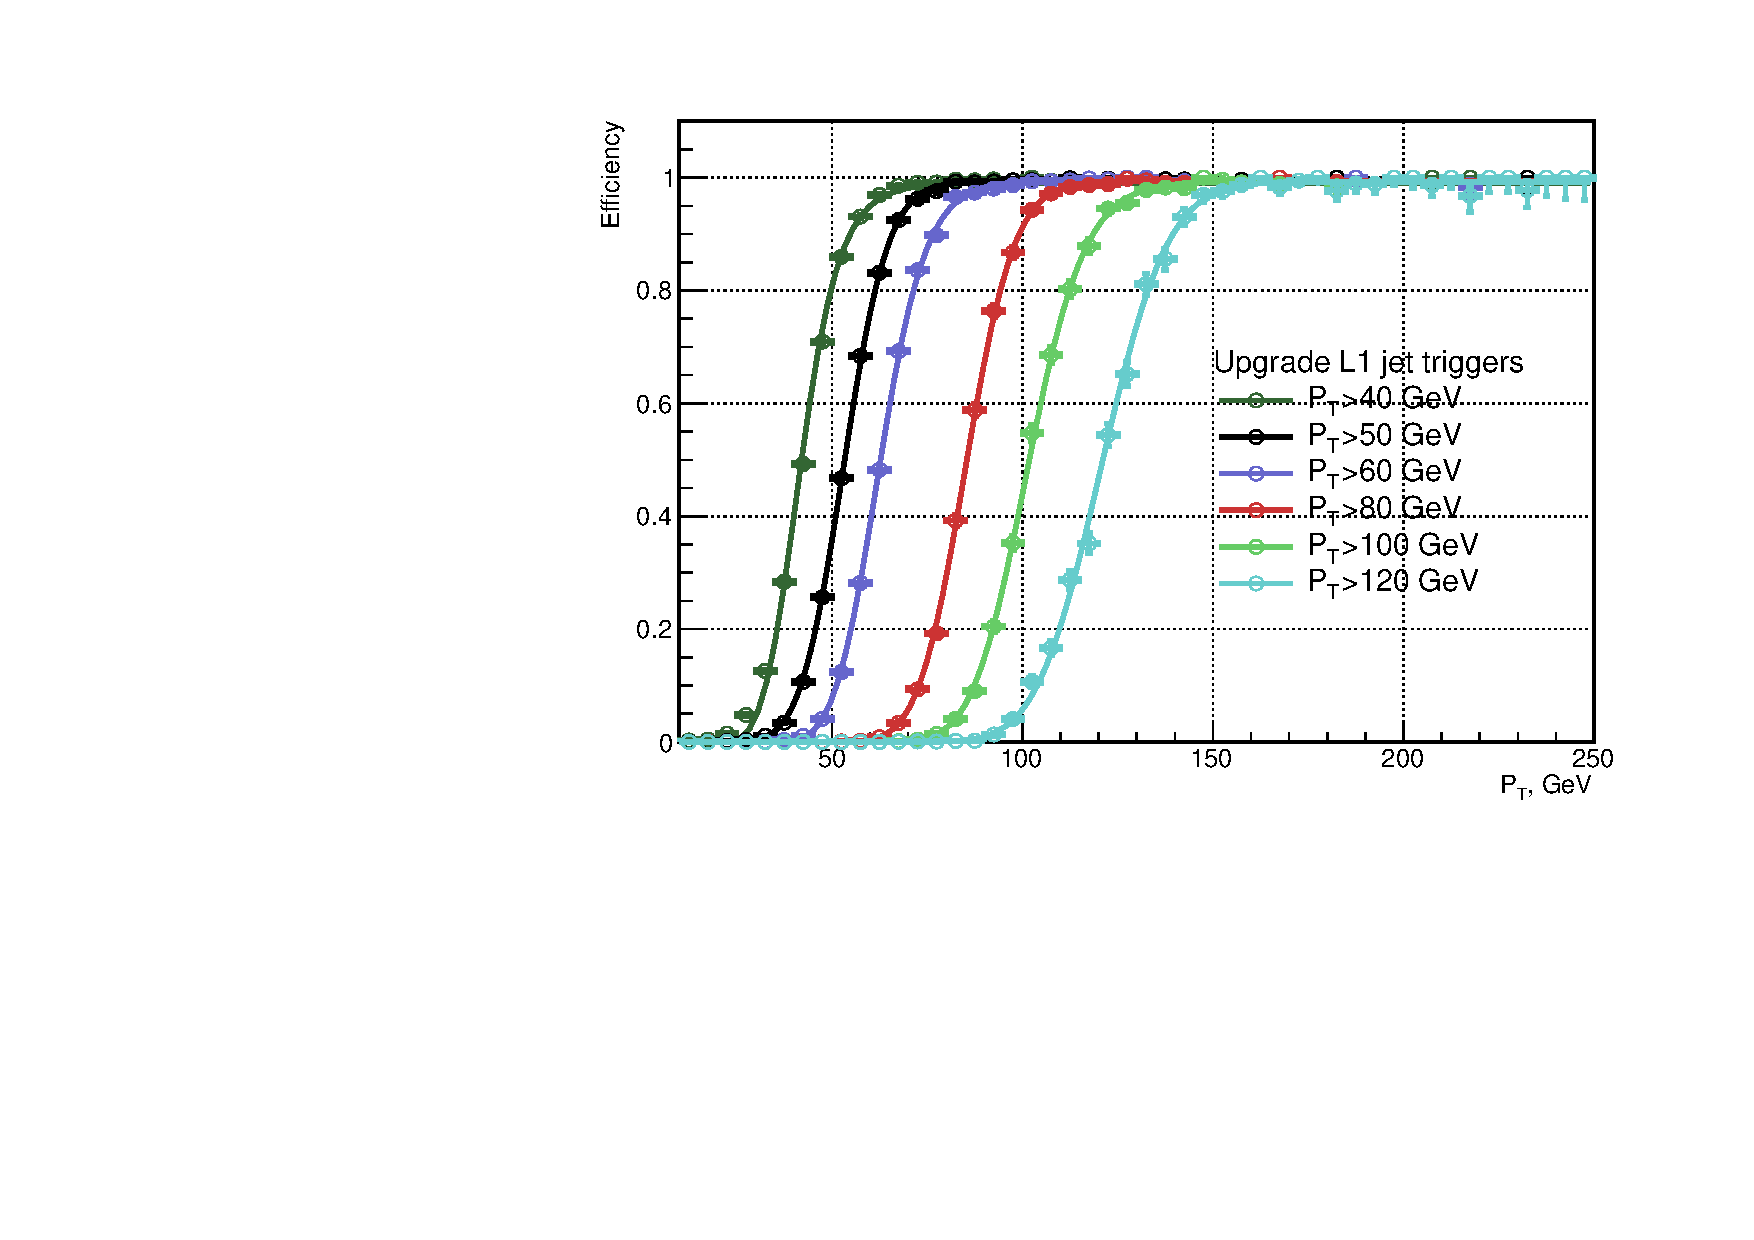
\includegraphics[scale=0.37]{Figures/l1jets//UpgradeL1JetTriggers.pdf}
\caption{On the left are the trigger turn on curves for the current jet algorithm and on the right are the trigger turn on curves for the upgrade jet algorithm, for various single jet trigger thresholds, and were calculated using relatively low \ac{PU} data.}
\label{JetTO_lowPU}
\end{center}
\end{figure}

\begin{figure}[t!]
\begin{center}
  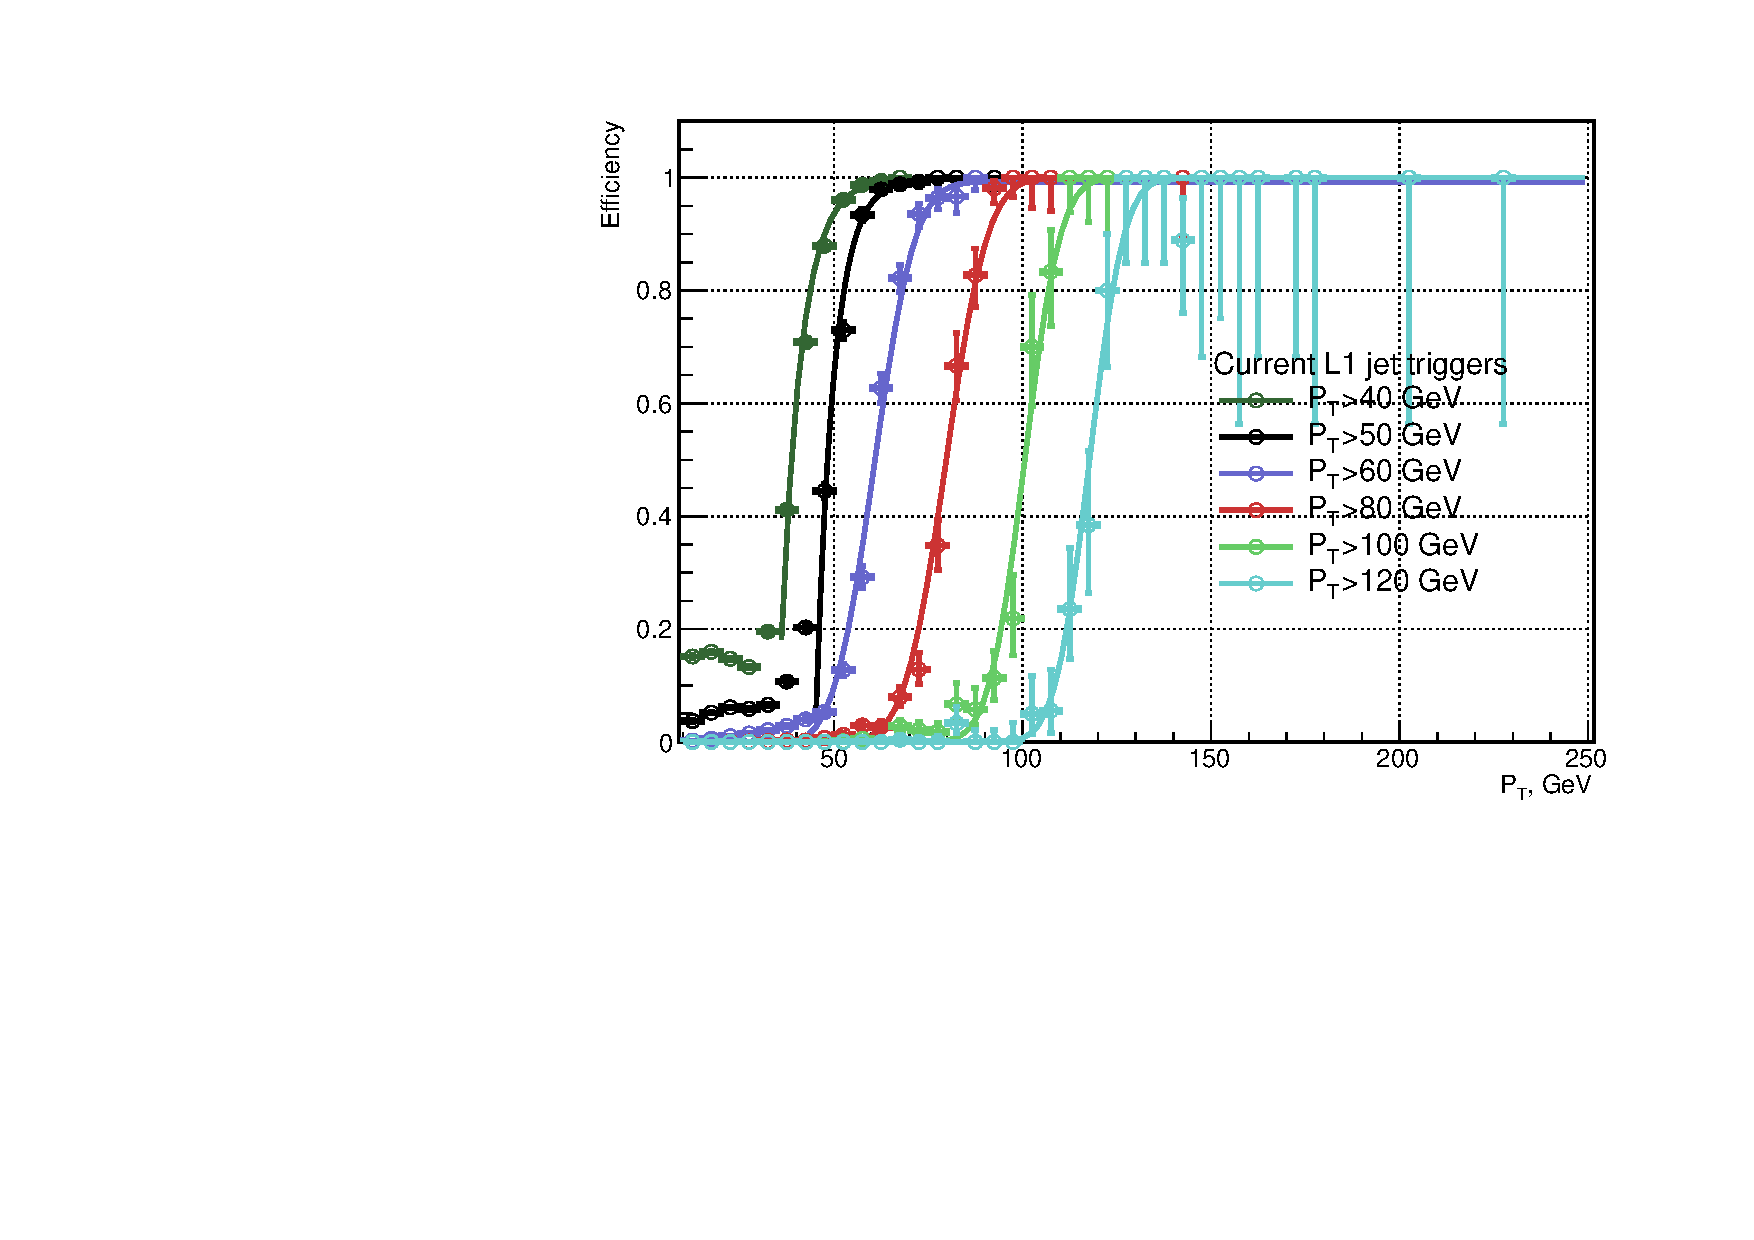
\includegraphics[scale=0.37]{Figures/l1jets//CurrentL1JetTriggersHPU.pdf}
    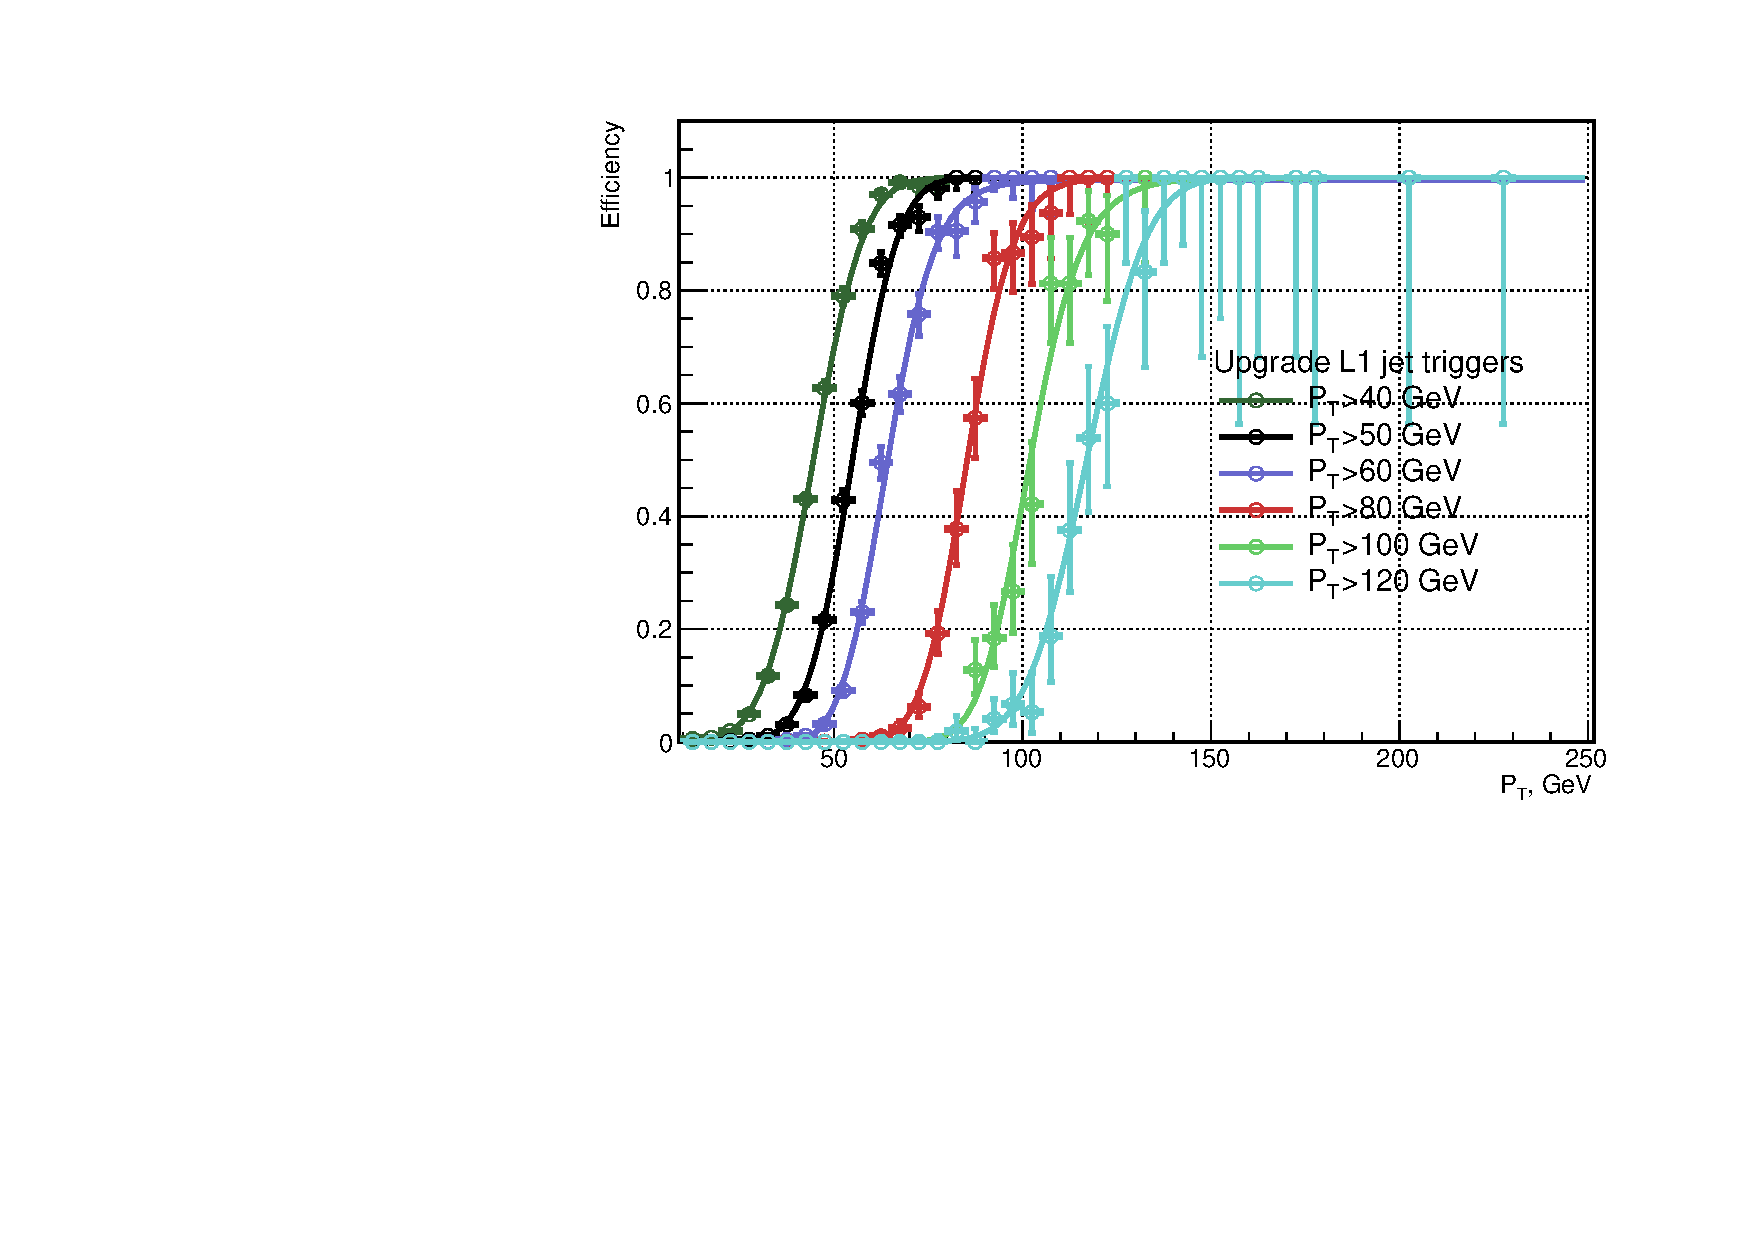
\includegraphics[scale=0.37]{Figures/l1jets//UpgradeL1JetTriggersHPU.pdf}
\caption{On the left are the trigger turn on curves for the current jet algorithm and on the right are the trigger turn on curves for the upgrade jet algorithm, for various single jet trigger thresholds, using relatively high \ac{PU} data.}
\label{JetTO_highPU}
\end{center}
\end{figure}

The \ac{PU} subtraction of the proposed upgrade algorithm is also evident in the upward shift in energy of the turn on curves, going from the current algorithm to the upgrade algorithm. 
For a requirement of, for example, one 40~\GeV jet at \ac{L1}, the offline value at which 95\% of events pass the 
trigger is 51.4~\GeV for the current algorithm in the high \ac{PU} dataset; and 62~\GeV for the upgrade algorithm.
Table~\ref{tab:trigTO} shows the offline transverse momentum value at which the trigger is 95\% efficient for the various turn on curves shown in Figure~\ref{JetTO_highPU}.
A lower typical hadronic energy at \ac{L1} in events reconstructed using the upgrade algorithm, 
due to the \ac{PU} subtraction, drives the 95\% efficiency values up.
Plateau efficiency values are 1 in both algorithms, meaning the upgrade jet algorithm (like the current algorithm) is fully efficient at large jet \pt values.

\begin{table}[htb]   
    \begin{center}
        \caption{The 95\% efficiency values for various \ac{L1} jet transverse momentum thresholds, in~\GeV, and plateau efficiency values for the current and upgrade algorithm, for turn on curves taken in high \ac{PU} data and shown in Figure~\ref{JetTO_highPU}.}\label{tab:trigTO}
        {%\small
            \begin{tabular}{c|cc|cc} 
            %\hline
 &   \multicolumn{2}{c|}{Current L1} &  \multicolumn{2}{c}{Upgrade L1} \\ \hline 
         L1 threshold  & 95\% efficiency & Plateau & 95\% efficiency & Plateau \\ \hline
         40  & 51.4 & 1 & 62.0 & 1 \\
         50  & 59.5 & 1 & 70.9 & 1 \\
         60  & 75.4 & 1 & 83.7 & 1 \\
         80  & 94.1 & 1 & 103  & 1 \\
        100  & 112.9 & 1 & 123.6 & 1 \\
            %\hline
            \end{tabular}
        } 
    \end{center}
\end{table}


\subsection{Jet trigger rates}
As discussed in Section~\ref{sec:LHCupgrade}, the purpose of building a new trigger is to be able to better 
control the trigger rates at reasonable energy thresholds in the future \ac{LHC} running, which is not possible with the current system. 
The projected trigger rates of the proposed jet algorithm in the next phases of \ac{LHC} running are therefore compared to the current system, in order to show the improvement in rates, and subsequent reduction in energy thresholds possible with the upgraded \ac{CMS} \ac{L1} calorimeter trigger.

Without any requirements on events that are recorded, i.e. when data is collected where no trigger has been applied, the rate is 
equivalent to the instantaneous luminosity multiplied by the inelastic proton-proton cross section, $R = L\times \sigma_{pp}$. 
In events where there are additional primary vertices in the bunch crossing, \ac{PU}$>1$, it takes the number of interacting vertices to get the process in question to occur, so there is an inverse proportionality to the \ac{PU}, $R = L\times \sigma_{pp}/PU$.
The rate of events to pass a particular trigger at \ac{L1}, $\text{R}_{\text{L1}}$, for a given luminosity and \ac{PU} scenario can then be written as
%
\begin{equation}
\text{R}_{\rm L1} = \text{R}_{\text{ev}} \cdot \frac{L\times \sigma_{pp}}{\ac{PU}},
\end{equation}
%
where $\text{R}_{\text{ev}}$ is the normalised trigger pass rate per event, which for a given set of events is simply the number of events passing a certain trigger divided by the total number of events.
%
Using this equation, the \ac{L1} trigger rates can then be extrapolated to a given luminosity and $\ac{PU}$ scenario.


The rates for several jet triggers are plotted in Figure~\ref{JetRate_L1}, in terms of the \ac{L1} jet energy.
%
Usually, the offline cut used in analysis is dictated by the allowed trigger rate, which corresponds to a particular \ac{L1} threshold, and therefore to a 95\% efficiency value - where the 95\% efficiency value is a low as possible to maintain as much phase space as possible (given the rate restrictions).
It is therefore also helpful to show the rate in terms of the 95\% efficiency, which enfolds both trigger rate and efficiency of the proposed algorithm and enables a fair comparison between the current and proposed upgrade algorithm.
The conversion from the online, \ac{L1} jet energy to offline 95\% threshold is taken from the turn on curves shown in Figure~\ref{JetTO_highPU}, using the linear conversion function shown in Figure~\ref{JetRate_conv}.
Figure~\ref{JetRate_95} shows the single and quad jet (where four jets are required) trigger rates vs the 95\% efficiency. 
The current and upgrade single jet rates are comparable, as the PU subtraction does very little to the leading jet in the event, whereas the multi jet triggers, such as the quad jet trigger, see a significant reduction in rate as PU jets are removed from the event.     

\begin{figure}[t!]
%\vspace{-1.cm}
\begin{center}
  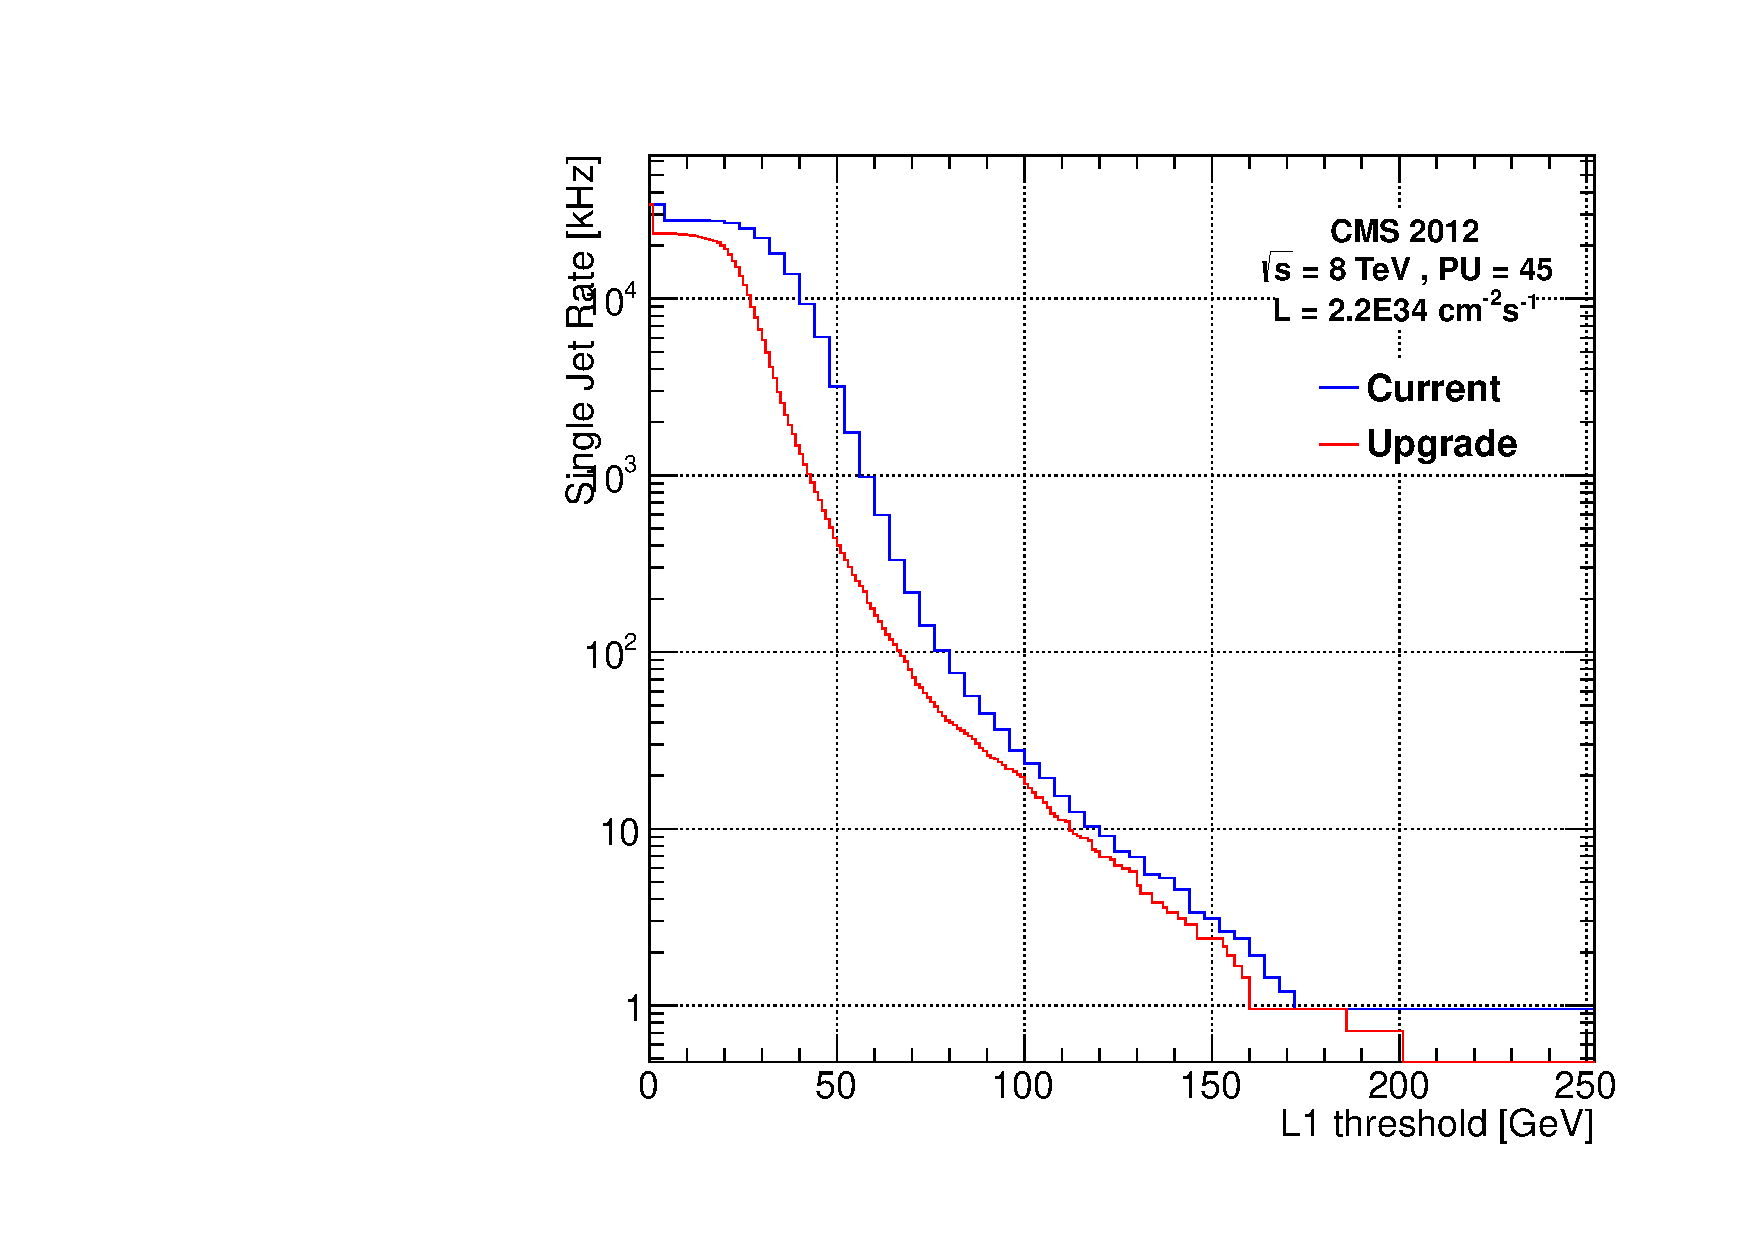
\includegraphics[scale=0.3]{Figures/l1jets/singleJetRates_2e34.pdf}
    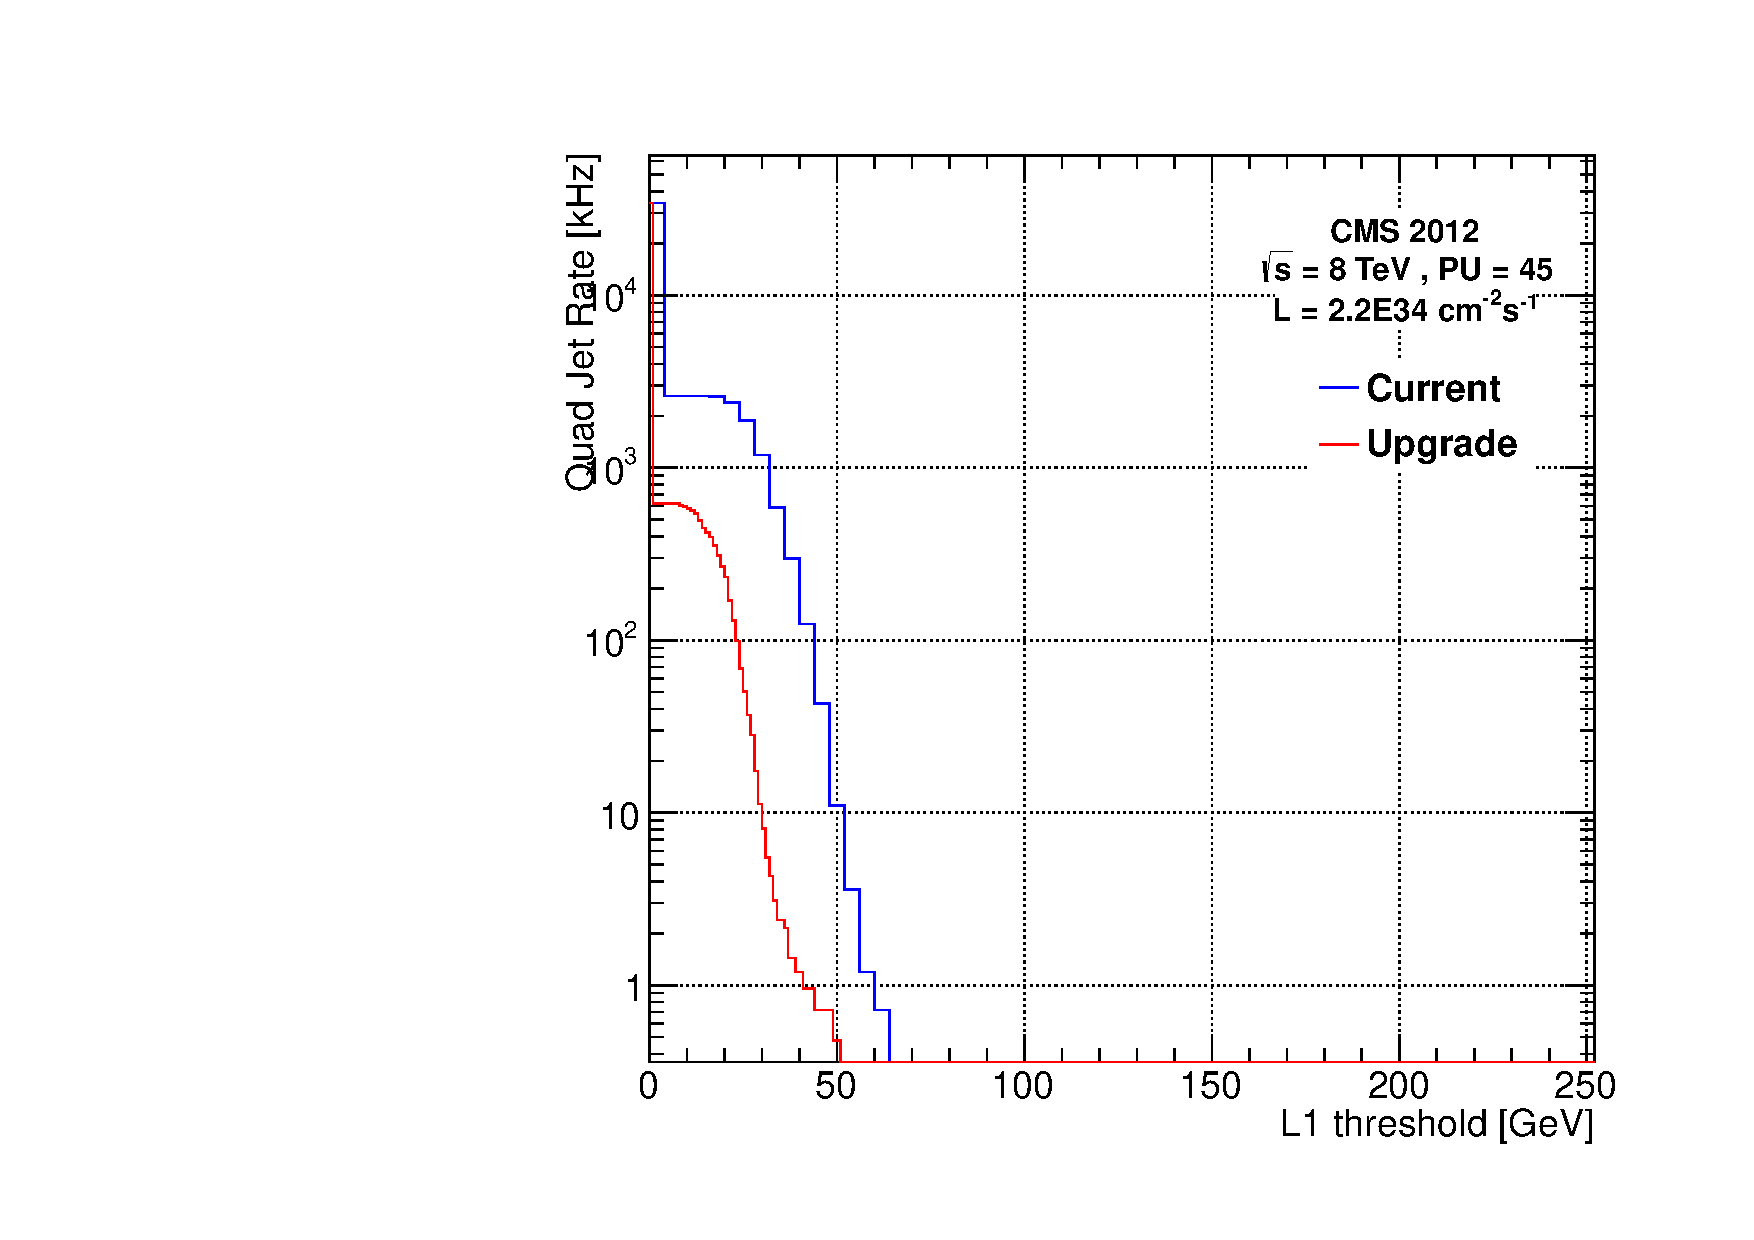
\includegraphics[scale=0.3]{Figures/l1jets/quadJetRates_2e34.pdf}
\caption{Rates of single and quad jet triggers. The single jet trigger shows similar performance to the current system, while the multi-jet trigger show a large reduction in rate}
\label{JetRate_L1}
\end{center}
\end{figure}

\begin{figure}[t!]
%\vspace{-1.cm}
\begin{center}
  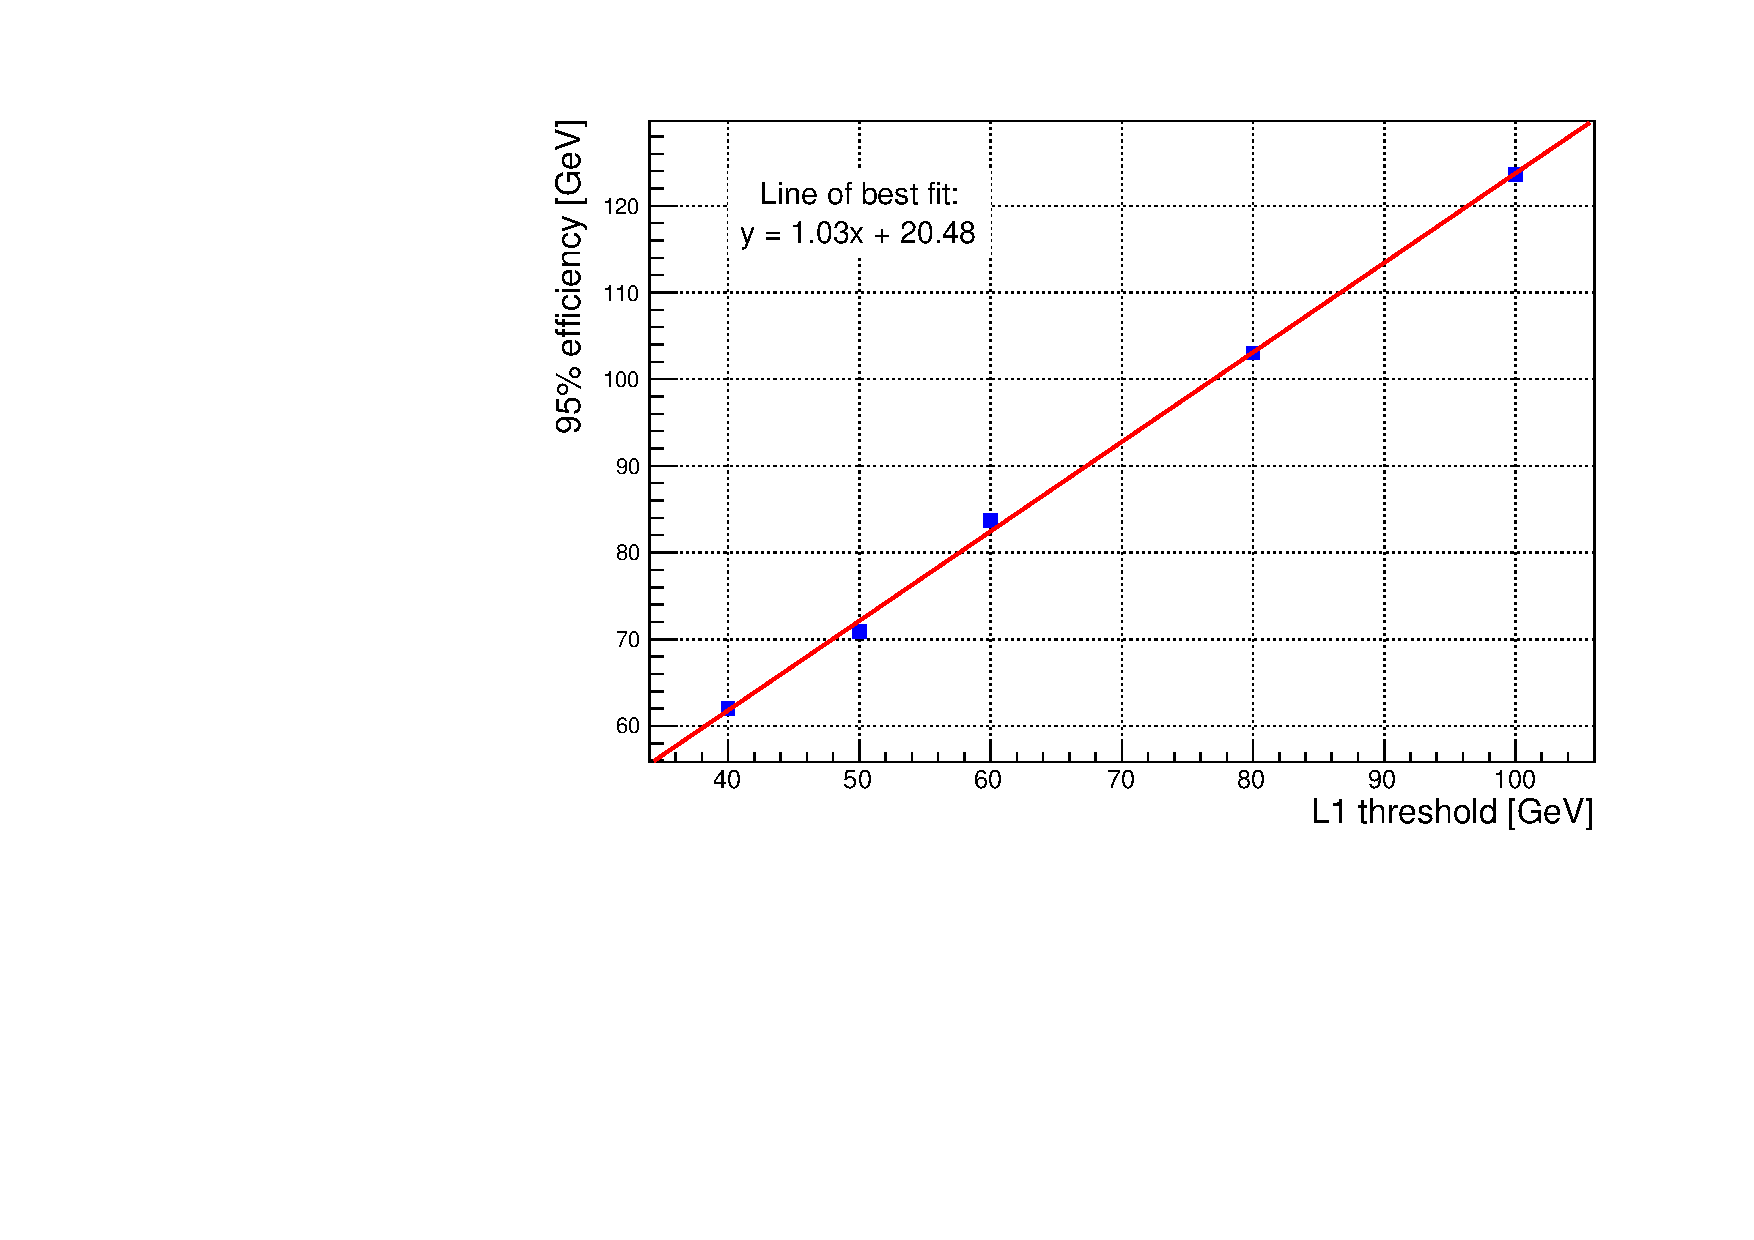
\includegraphics[scale=0.37]{Figures/l1jets/makePlot/jet_95threshold_conv.pdf}
\caption{Conversion between the \ac{L1} jet threshold and the 95\% efficiency as measured offline, for the proposed upgrade jet algorithm, using the turn on curves shown in Figure~\ref{JetTO_highPU}. }
\label{JetRate_conv}
\end{center}
\end{figure}

\begin{figure}[t!]
%\vspace{-1.cm}
\begin{center}
  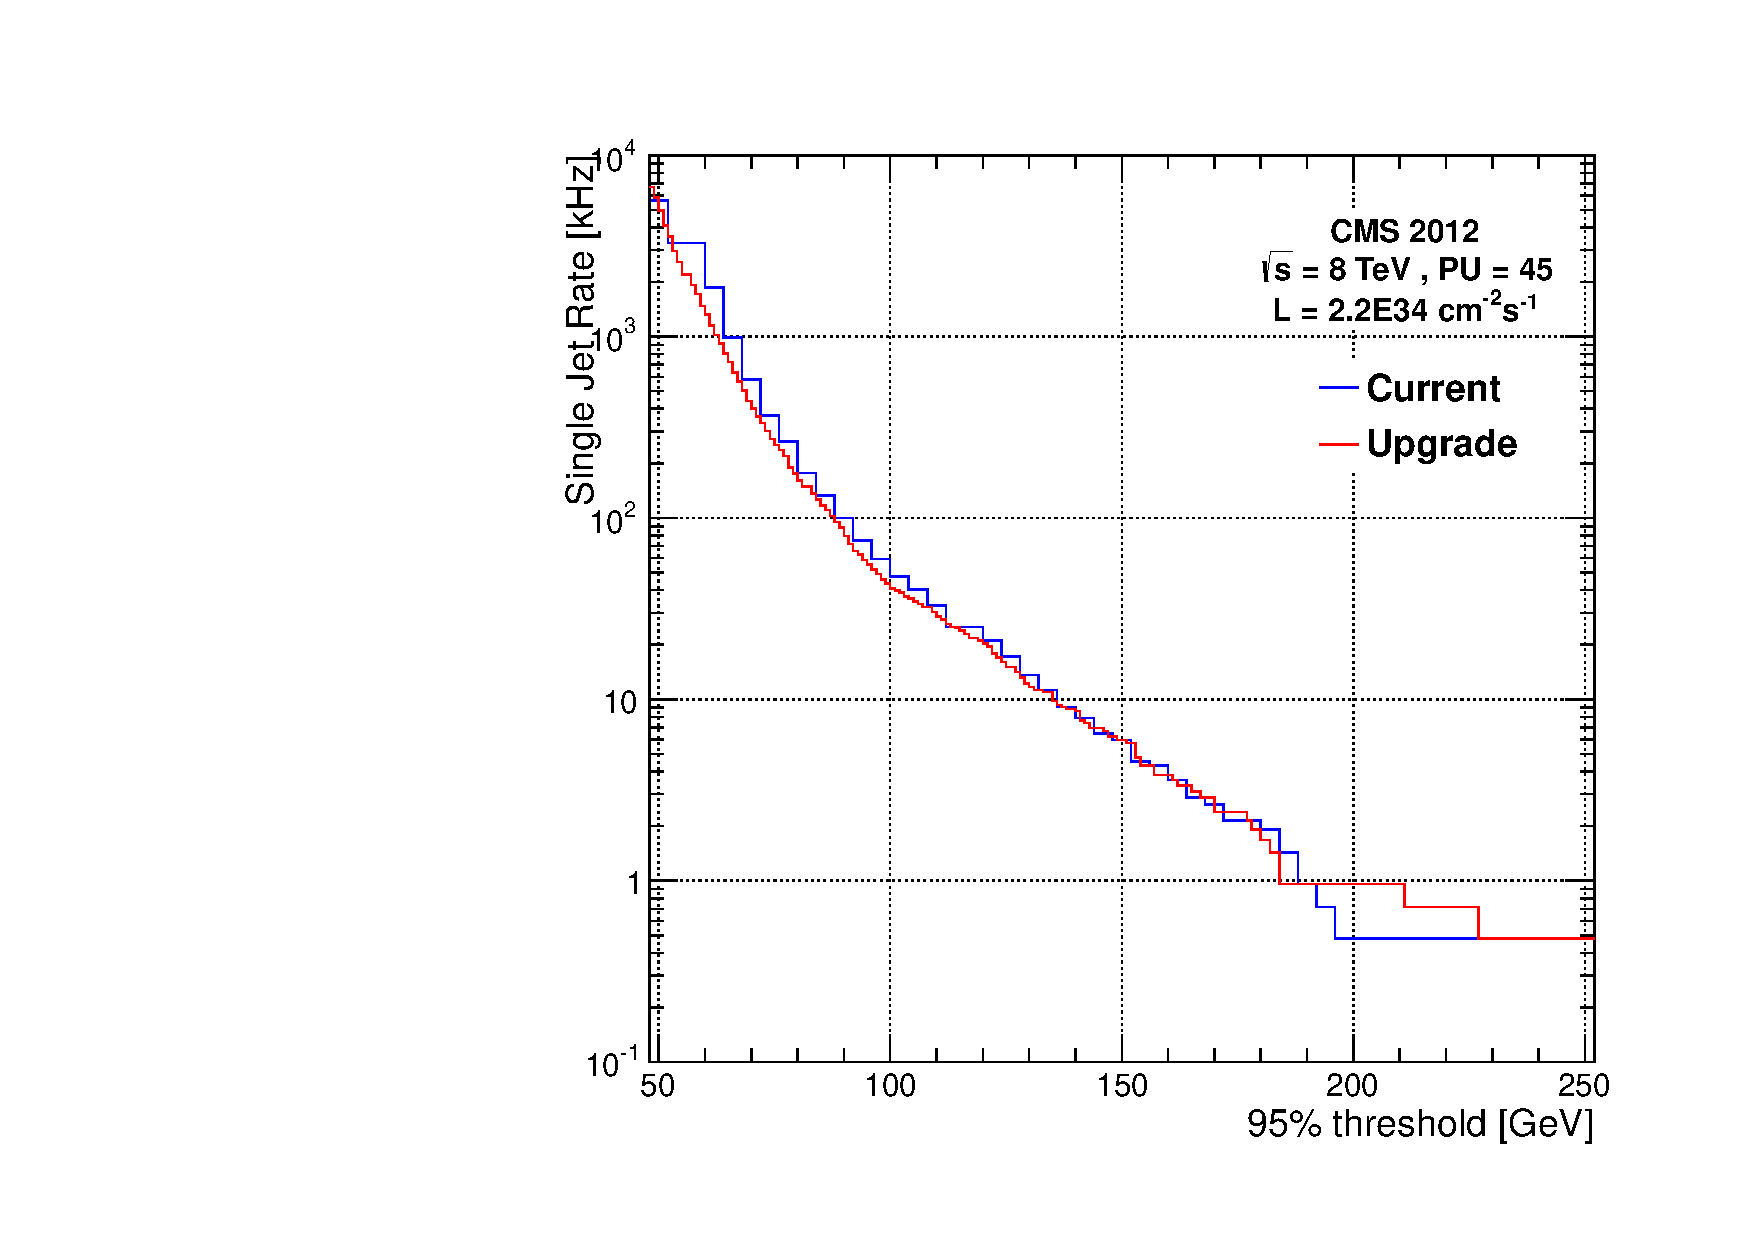
\includegraphics[scale=0.3]{Figures/l1jets/singleJetRates_95thresh_2e34.pdf}
    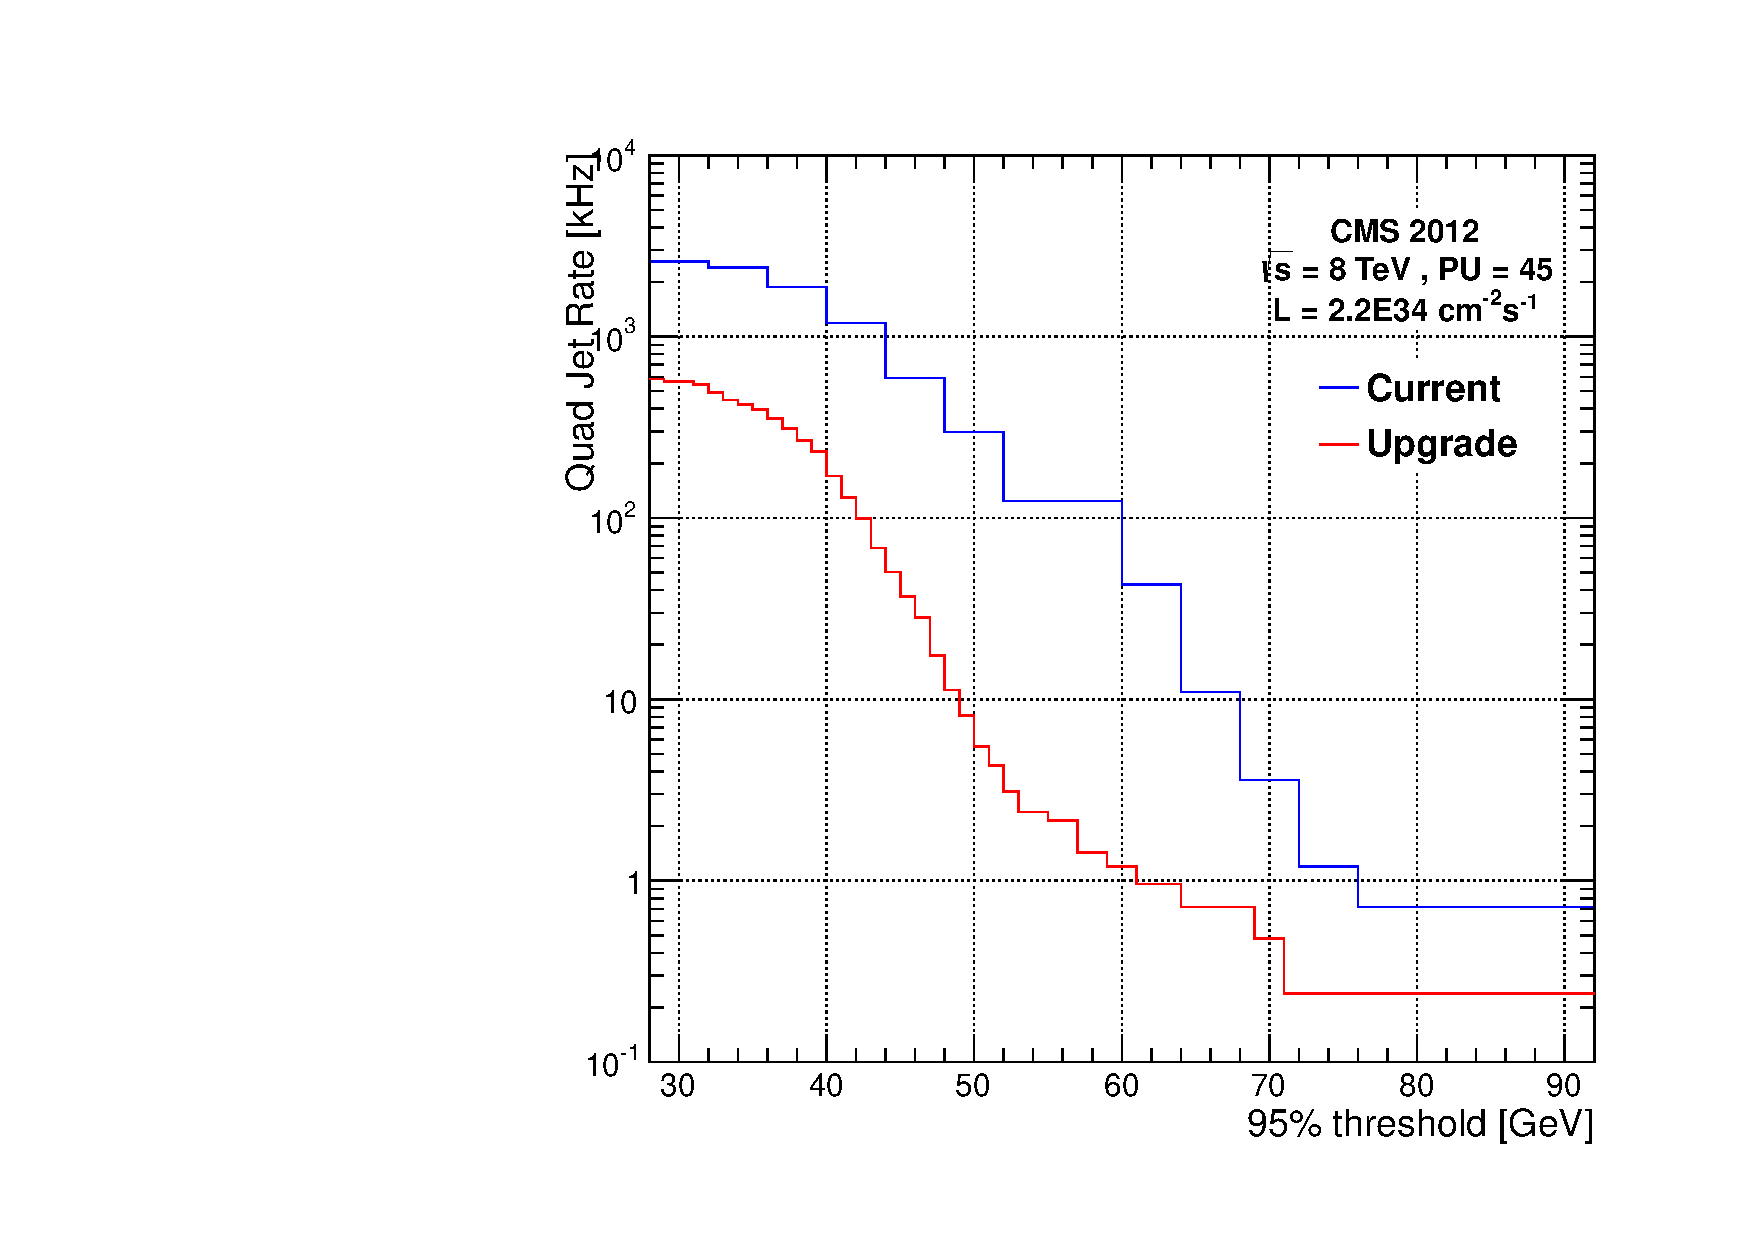
\includegraphics[scale=0.3]{Figures/l1jets/quadJetRates_95thresh_2e34.pdf}
\caption{Rates of single and quad jet triggers. The single jet trigger shows similar performance to the current system, while the multi-jet trigger show a large reduction in rate}
\label{JetRate_95}
\end{center}
\end{figure}


\subsection{Other jet variables}
Other offline variables, constructed from jets, have been widely used in the data analyses at \ac{CMS} at 7 and 8~\TeV, both at trigger level and offline.
They therefore also will also benefit from the upgraded calorimeter trigger, and shown here are the improvements in rates for \HT, the transverse hadronic energy which is defined as the scalar sum of jet transverse momenta in each event:
%
\begin{eqnarray}
\HT &=& \sum{|\pt^{\text{ jet}}|} %\\ 
%\MHT &=&  \sum{\ptv^{\text{ jet}}},
\end{eqnarray}  
where the sum is over all jets in each event.
\HT is commonly used for analysis which search for \ac{SUSY}, for example in Ref.~\cite{alphaT}.
It gives a good indication of the amount of hadronic energy in an event and so the energy transfer in the original inelastic p-p collision, which should be high for new physics processes to occur.
It is particularly sensitive to the number of primary vertices in each bunch crossing, as soft \ac{PU} jets are included in the sum.
The addition of \ac{PU} subtraction on an event-by-event basis in the proposed upgrade jet algorithm therefore has the potential to lead to significant improvements in the rate.
The trigger turn on curves for various \HT thresholds using the upgrade jet algorithm are shown in Figure~\ref{HTRate_conv} together with the conversion between the \ac{L1} threshold and the 95\% offline efficiency. 
The trigger rate of the \HT in terms of both the \ac{L1} threshold and the 95\% efficiency are shown in Figure~\ref{HTRate}, which shows a rate reduction of nearly an order of magnitude when using the upgrade algorithm compared to the current algorithm, in terms of the 95\% efficiency. 
This is a much fairer comparison between the two algorithms than the rate in terms of the \ac{L1} threshold, as the current \HT and \MHT values at \ac{L1} are not corrected to the jet energy scale.


\begin{figure}[t!]
%\vspace{-1.cm}
\begin{center}
  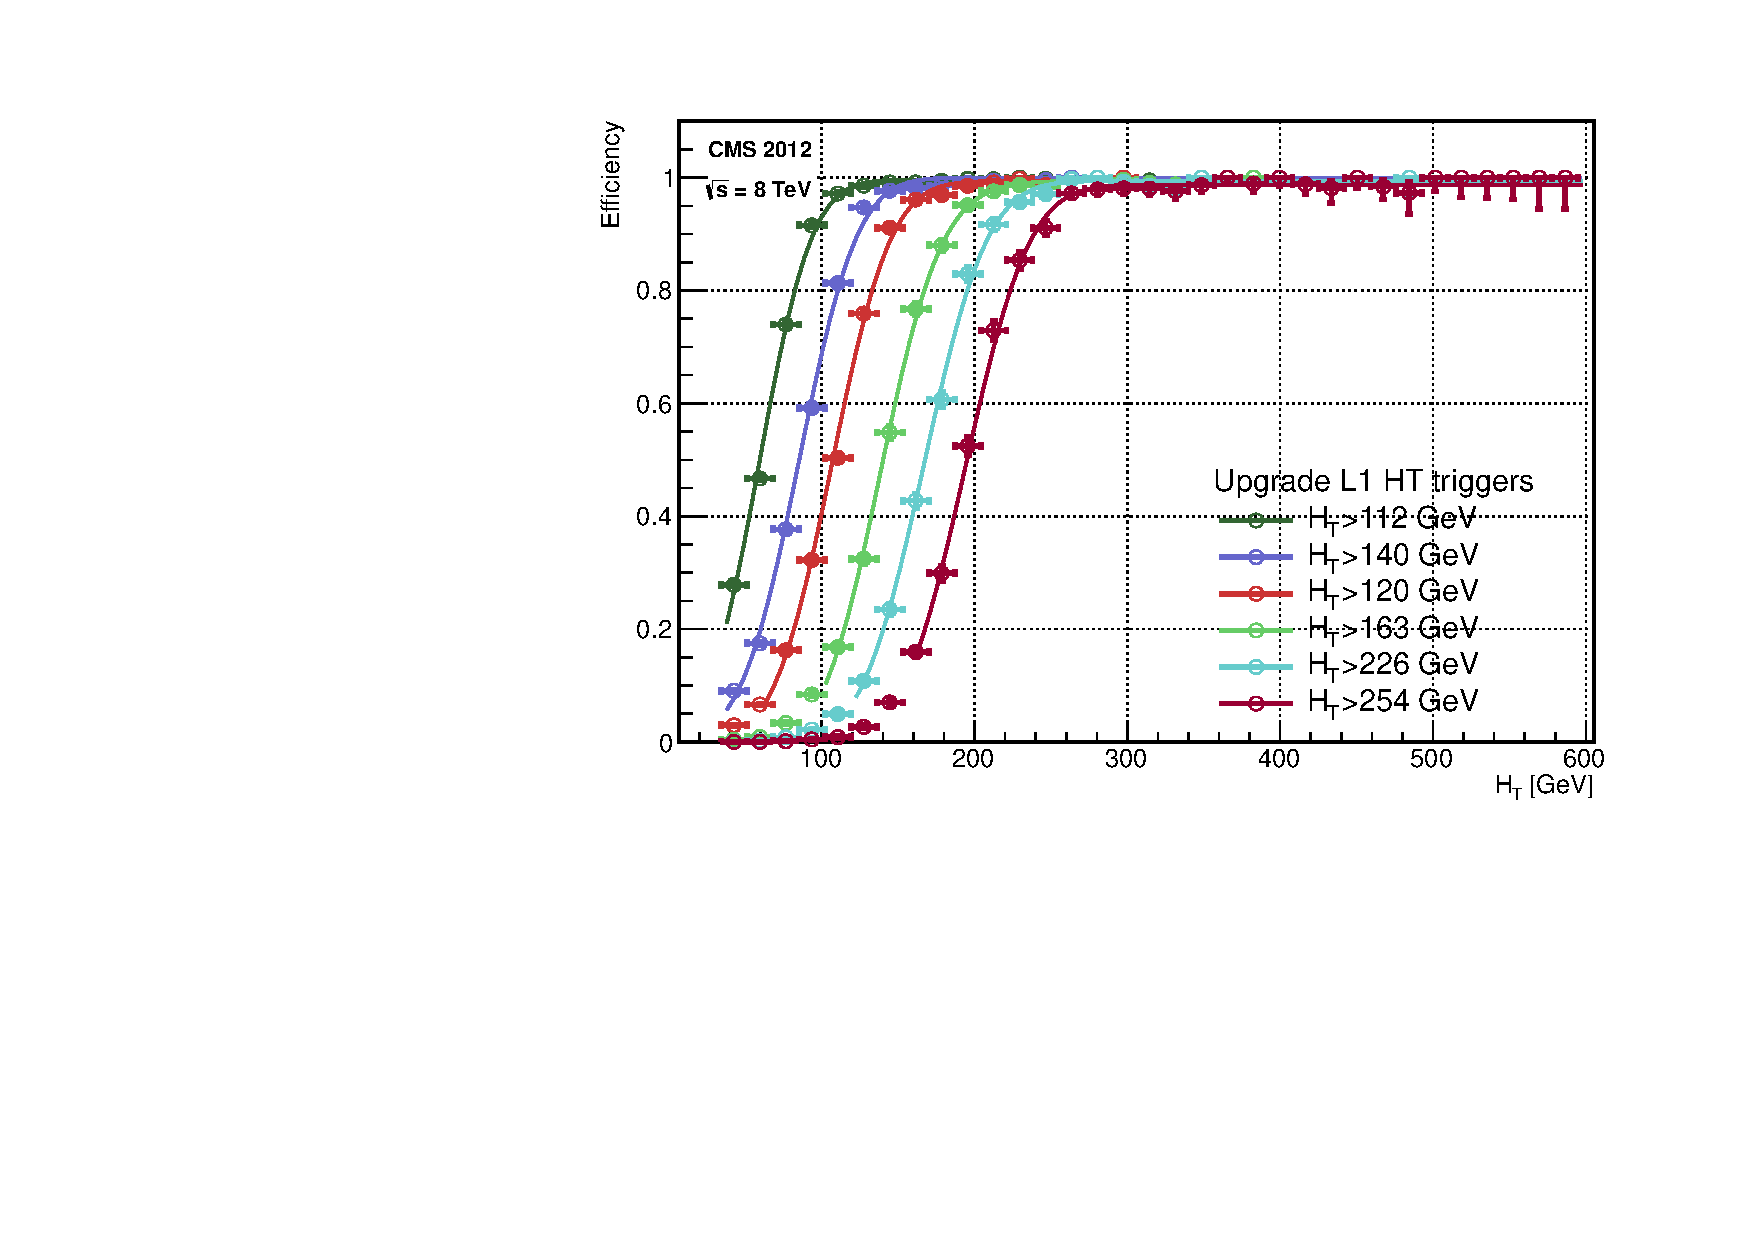
\includegraphics[scale=0.37]{Figures/l1jets/UpgradeL1HTTriggersfixed.pdf}
  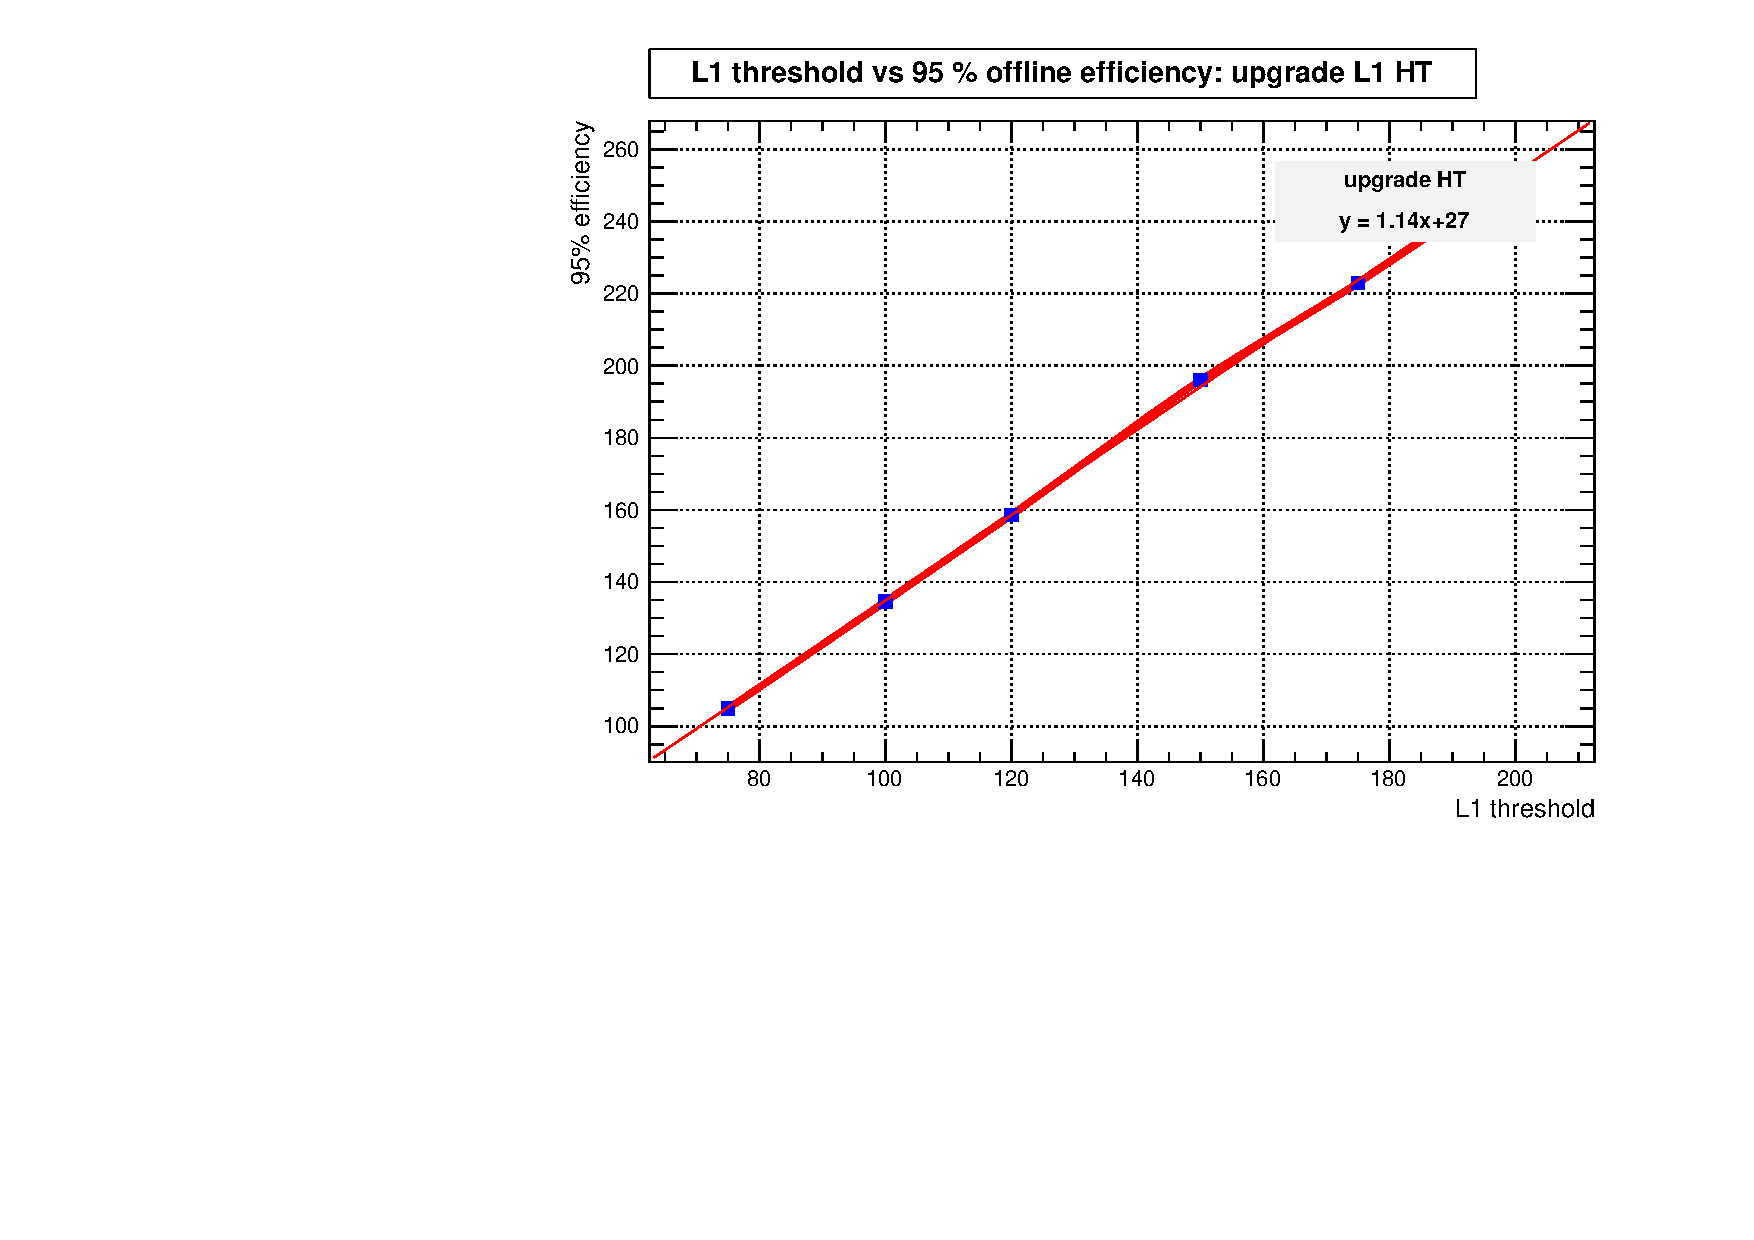
\includegraphics[scale=0.37]{Figures/l1jets/upgradeHTconv.pdf}
\caption{The trigger turn on curves for the \HT variable, left, and the conversion between the \ac{L1} \HT threshold and the 95\% efficiency as measured offline, using \HT constructed with the proposed upgrade algorithm. }
\label{HTRate_conv}
\end{center}
\end{figure}

\begin{figure}[t!]
%\vspace{-1.cm}
\begin{center}
  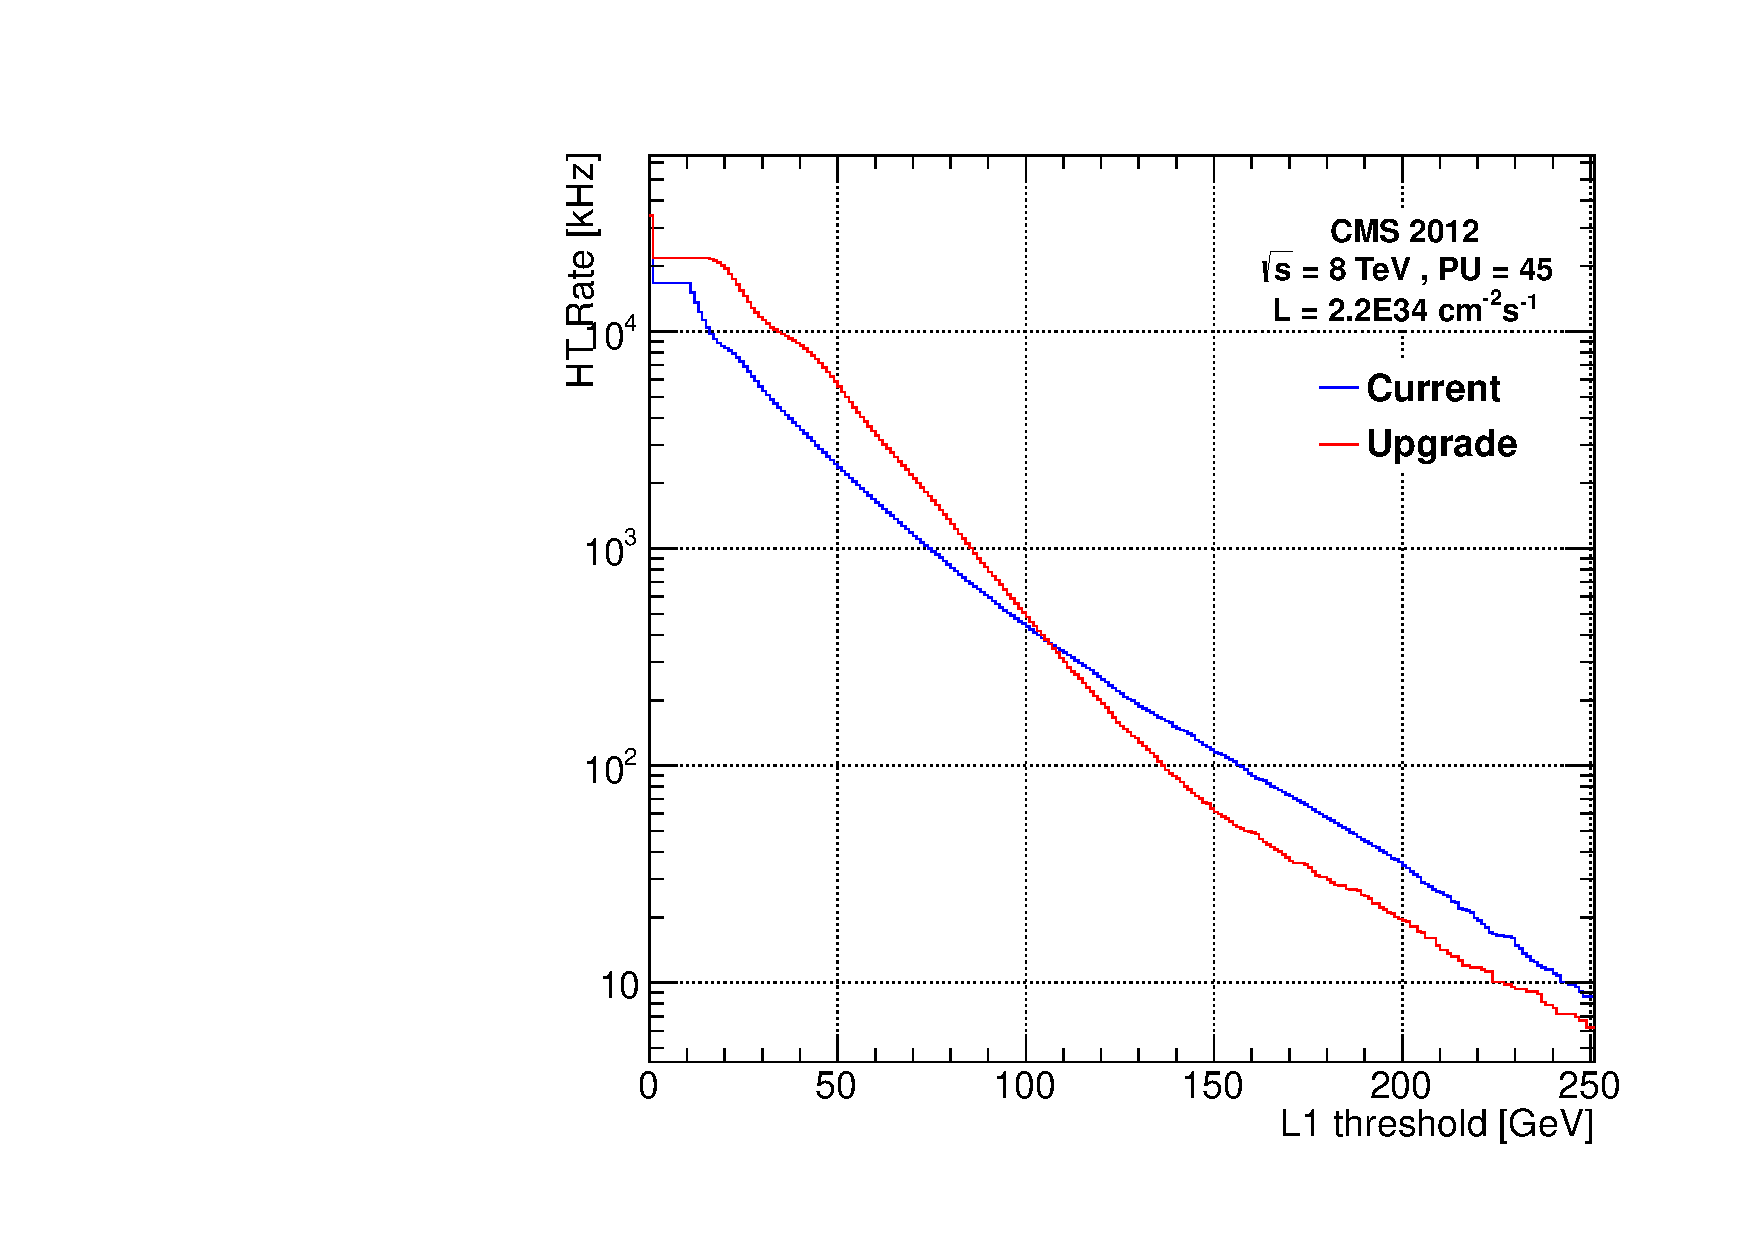
\includegraphics[scale=0.3]{Figures/l1jets/HTRates_2e34.pdf}
    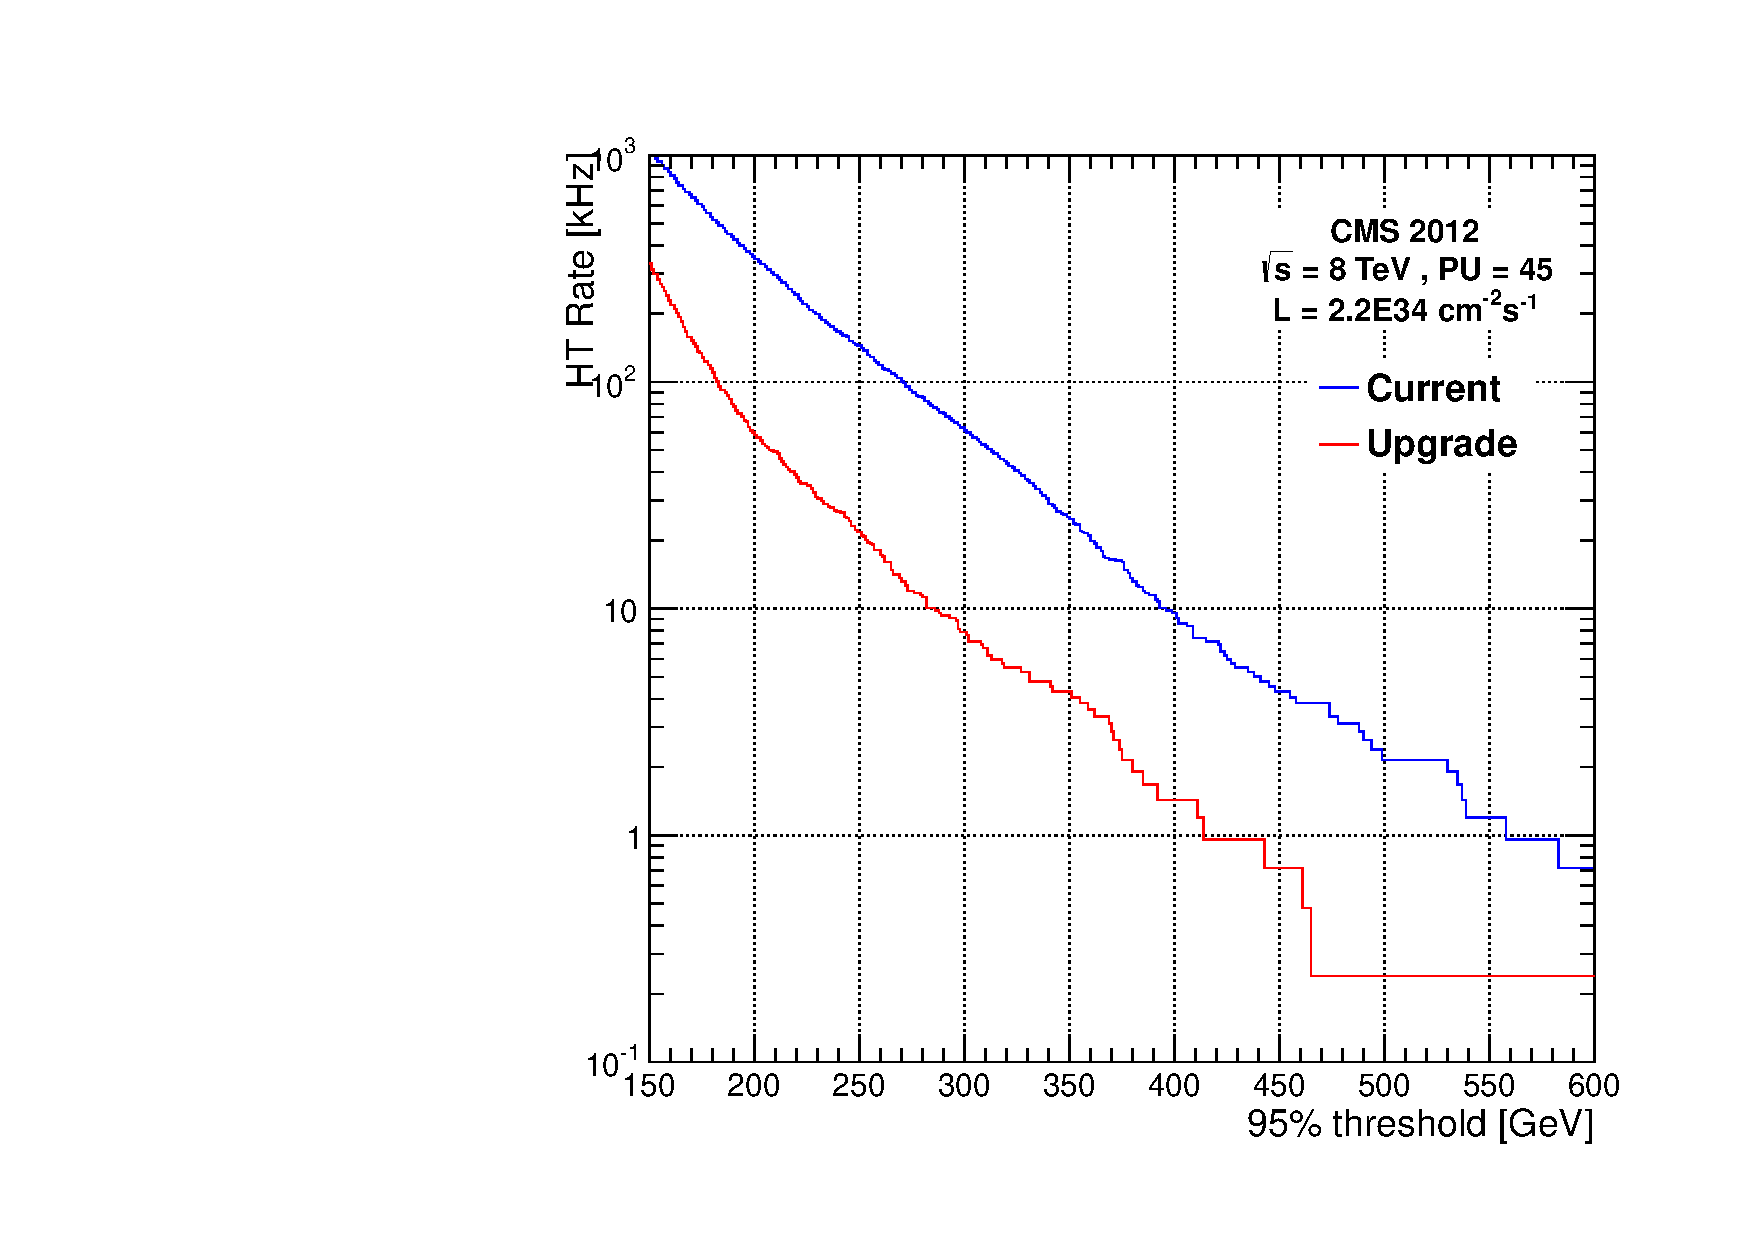
\includegraphics[scale=0.3]{Figures/l1jets/HTRates_95thresh_2e34.pdf}
\caption{Rates of \HT triggers, vs L1 threshold (left) and 95\% offline threshold (right), where the conversion between L1 threshold and 95\% efficiency is taken from Figure~\ref{HTRate_conv}. There is a significant reduction in rates with the proposed upgrade algorithm.}
\label{HTRate}
\end{center}
\end{figure}

% The expected enhancement in \MHT is less significant, because it is defined as a vector sum so therefore already has a rudimentary \ac{PU} subtraction applied. 
% However, the rates were nevertheless investigated, and are shown in Figure~\ref. 
 

\section{Conclusion}
The proposed upgrade jet algorithm, possible to implement with the upgraded \ac{CMS} calorimeter trigger based upon a \ac{TMT} architecture, shows significant improvements over the current \ac{L1} jet algorithm.
By utilising event-by-event \ac{PU} subtraction at \ac{L1} for the first time, the dependency of \ac{PU} of the \ac{L1} jet algorithm is much reduced.
By taking advantage of the full tower level granularity of the calorimeter, the angular resolutions of the algorithm are also much improved.
While similar trigger rates are seen for the single jet triggers, there are big improvements in the multijet trigger rates; and a factor of two reduction in the quad-jet trigger rate.
The \HT variable also sees a factor 10 reduction in rate.
These rate reductions will allow lower energy thresholds in the upgraded \ac{CMS} \ac{L1} calorimeter trigger, as compared to the current \ac{L1} jet algorithm, and help to maintain the energy thresholds and jet rates that were used in 7 and 8~\TeV data taking.


This upgrade jet algorithm was proposed in~\cite{Tapper:1556311}, and the majority work was done during 2012. 
Many more improvements to the algorithm are possible, using different \ac{PU} subtraction techniques, different jet shapes, and additional parameters.
Indeed, since this work was completed such improvements have been made, and documented elsewhere~\cite{newL1jetWork}.


  \graphicspath{Figures/sus13009}

\chapter{Searching for SUSY with compressed mass spectra using monojet events}
\label{chap:sus13009}

\chapterquote{Physics, as we know it, will be over in six months.}
{(1928) Max Born, 1882 -- 1970}


This chapter and the next describe a search for events containing a single energetic jet and missing transverse momentum, 
using a data sample collected at 8~\TeV by the \ac{CMS} detector at the \ac{CERN} \ac{LHC} and corresponding to an integrated luminosity of 19.7~\fbinv.
In this chapter, we describe the event selection of the search as well as background estimations and the associated systematic uncertainties.



\section{Introduction}


The monojet signature of a high \pt jet and an imbalance of momentum in the transverse plane is the discovery signal for many new physics scenarios that have genuine missing energy in the final state. 
Searches for Large Extra Dimensions in the framework of the \ac{ADD} model~\cite{ADDextraDimensions}, 
for \ac{DM} using effective field theory and simplified models, 
and Unparticle production~\cite{bib:Delgado} have been presented in previous searches both at the LHC and the Tevatron~\cite{Abazov:2008kp,Aaltonen:2008hh,Aaltonen:2012jb,Aad:2011xw,ATLAS:2012ky,bib:CMS_EXO11003,bib:CMSEXO11059,bib:CMSEXO12048}
using the monojet channel.
Signals are commonly invisible; for example the theorized \ac{DM} is a \ac{WIMP} candidate, and as such, does not interact with any part of the detector.
It therefore leaves no signal but an imbalance of momentum in the transverse plane, which is balanced by an \ac{ISR} particle. 
In this case, the \ac{ISR} particle is a quark or gluon, leading to a high \pt jet. 
Searches have also been conducted using other radiated particles: photons (termed ``monophoton'') and \W or \Z bosons (``mono-W'' or ``mono-Z'')~\cite{monophoton1,monophoton2,monophoton3,monophoton4, Aaltonen:2008hh,monophoton5,monophoton6,monophoton7}.
However, because monojet searches have the advantage of higher production cross sections (as the strong coupling constant $\alpha_{s}$ is greater than the electromagnetic or weak coupling constants), they typically lead to stronger limits.

A search for compressed \ac{SUSY} in the third generation is motivated in Chapter~\ref{chap:theory}.
Such signals are slightly different: Feynman diagrams are shown in Fig.~\ref{fig:feynmandiagrams}. 
The final state does not just consist of missing transverse momentum balanced by an ISR jet; 
there are also sparticle decay products.
These are therefore not pure monojet signals.
However, when the mass difference between the parent sparticle and the \ac{LSP} decreases below 80~\GeV, decay products become increasingly soft
and indistinguishable from \ac{SM} backgrounds.
Events that have an energetic \ac{ISR} jet produced in association with parent sparticles, which recoils against the missing transverse momentum due to the LSP leaving the detector (``boosted events''),
provide a clear signature in such scenarios.
One high \pt jet alongside large \MET give rise to a monojet final state, in events where the soft sparticle decay products are too soft to observe.


Searches are for the pair production of top squarks (\sTop\santiTop) that decay to charm quarks and the LSP, \ttwocc, and bottom squarks (\sBot\santiBot) that decay to bottom quarks and the LSP, \ttwobb.
By selecting events using particles produced alongside \sTop\santiTop or \sBot\santiBot, the search is sensitive to mass differences of less than 10~\GeV.
The search presented here is a re-optimization of the well-established search detailed in Refs.~\cite{bib:CMSEXO12048,bib:CMS_EXO11003,bib:CMSEXO11059}, performed by the author as part of the CMS monojet group.
By modifying the search criteria to cut out the soft jets, sensitivity to compressed mass spectra is achieved.


\begin{figure}[!Hhtb]
  \begin{center}
 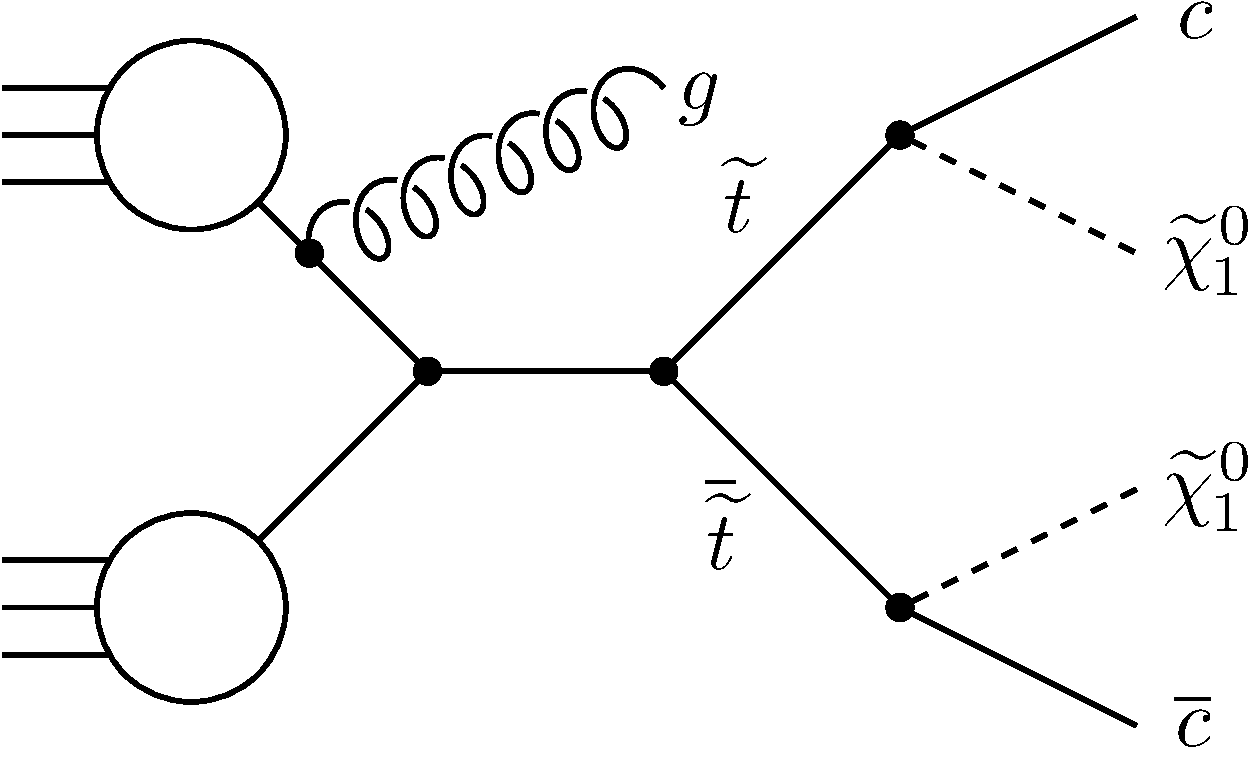
\includegraphics[scale=0.4]{Figures/sus13009/t2cc.pdf}
 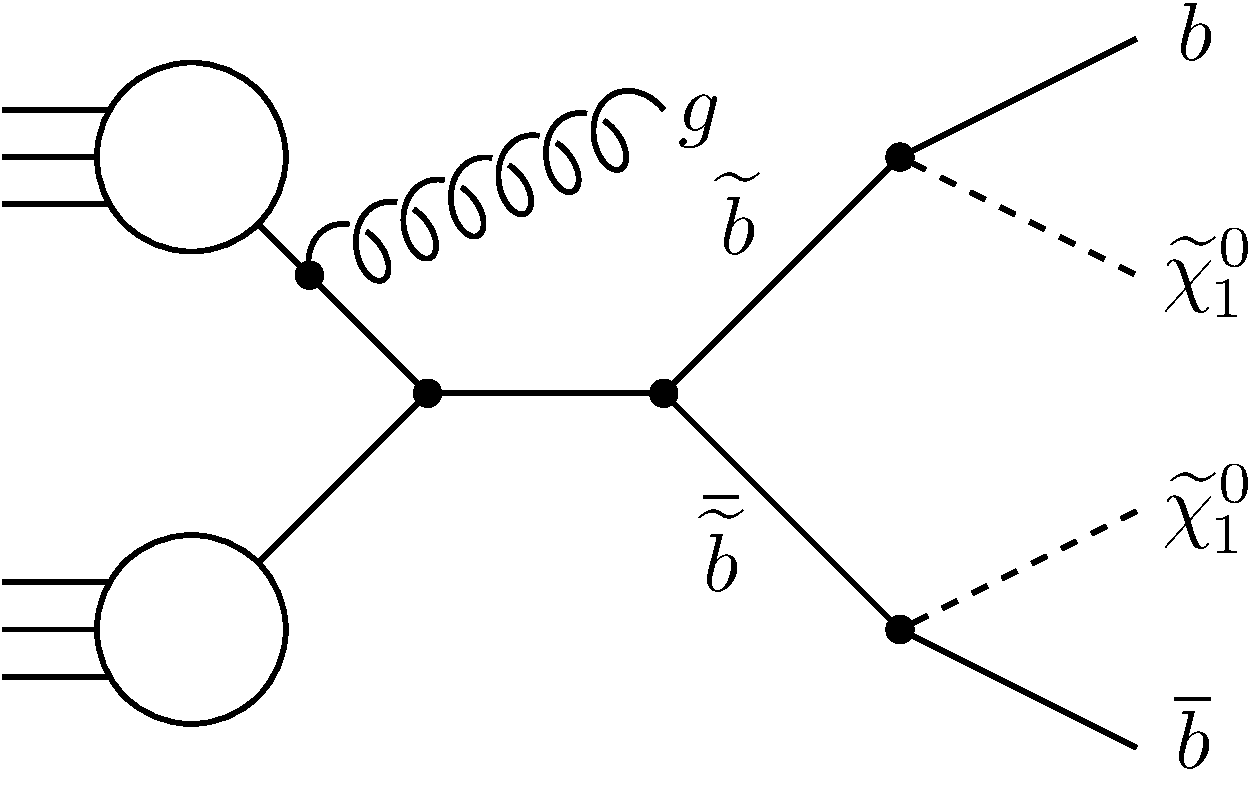
\includegraphics[scale=0.4]{Figures/sus13009/t2bb.pdf}
  \caption{Feynman diagrams of the signals probed. The top diagram shows the \ac{FCNC} process \ttwocc and the bottom diagram shows the process \ttwobb. In both cases, an \ac{ISR} gluon leads to an energetic jet, and balances the \MET due to \ac{LSP}s escaping the detector leaving no trace.}
	         \label{fig:feynmandiagrams}
  \end{center}
\end{figure}



%




\section{Data samples}
\label{sec:data}

The data for this search were collected using a combination of two triggers at the \ac{HLT}. 
The first requires events to have $\MET>120$~\GeV.
The second, a dedicated monojet trigger, requires a central jet ($|\eta|<2.6$) with $\pt>80~\GeV$ and \MET 
(calculated without muons) to be greater than 95 or 105~\GeV. 
These triggers also have coarse noise cleaning filters applied. 
The first has various requirements on the energy deposits in the \ac{HCAL} to cut out noisy events, 
and the second demands that the neutral energy deposited in the \ac{ECAL} is less than 95\% of the total energy deposited.
They are seeded by \ac{L1} triggers which require the missing transverse momentum, calculated using \ac{L1} seeds and in \ac{L1} energy units, to be greater than 36, 40 or 50 for the first trigger, or greater than 40 for the second trigger. 


Very few events with \MET below 100 GeV, where it is calculated offline using optimal object reconstruction,  will pass the analysis triggers described above that require \MET calculated online to be above 120~\GeV, or to be above 95 or 105~\GeV without muons. 
However, most events with \MET (reconstructed offline) above 200~\GeV will pass the same analysis triggers. 
It is therefore necessary to calculate the efficiency of these triggers in terms of the key analysis variables, \MET and the \pt of the leading jet, in order to find where best to place offline analysis cuts. 
An independent sample of events collected using a trigger requiring a single isolated muon with $\pt > 24$ and $|\eta|<2.4$ is used.
The efficiency is given by the ratio of the number events passing the analysis triggers to the number of events passing the reference trigger. 
It is shown in the trigger turn-on curves in Figure~\ref{fig:trigger-1D} as a function of \MET\ and the \pt\ of the leading jet, as reconstructed offline. 
Here, the different colours show the different runs of the \ac{LHC} during Run I.
The dedicated monojet trigger described above was introduced for Run C, which increased the efficiency of the combination of the triggers for lower values of \MET and leading jet \pt compared to Runs A and B. 
%A two-dimensional plot of the trigger efficiency is shown as a function of the \MET\ and leading jet \pt\ in Figure~\ref{fig:trigger-2D}. 
The plots in Figure~\ref{fig:trigger-1D} show that the trigger paths become almost 100\% efficient at $\pt(j_1)\sim110~\GeV$ and $\MET\sim220~\GeV$.

\begin{figure}%[!Hhtb]
  \begin{center}
 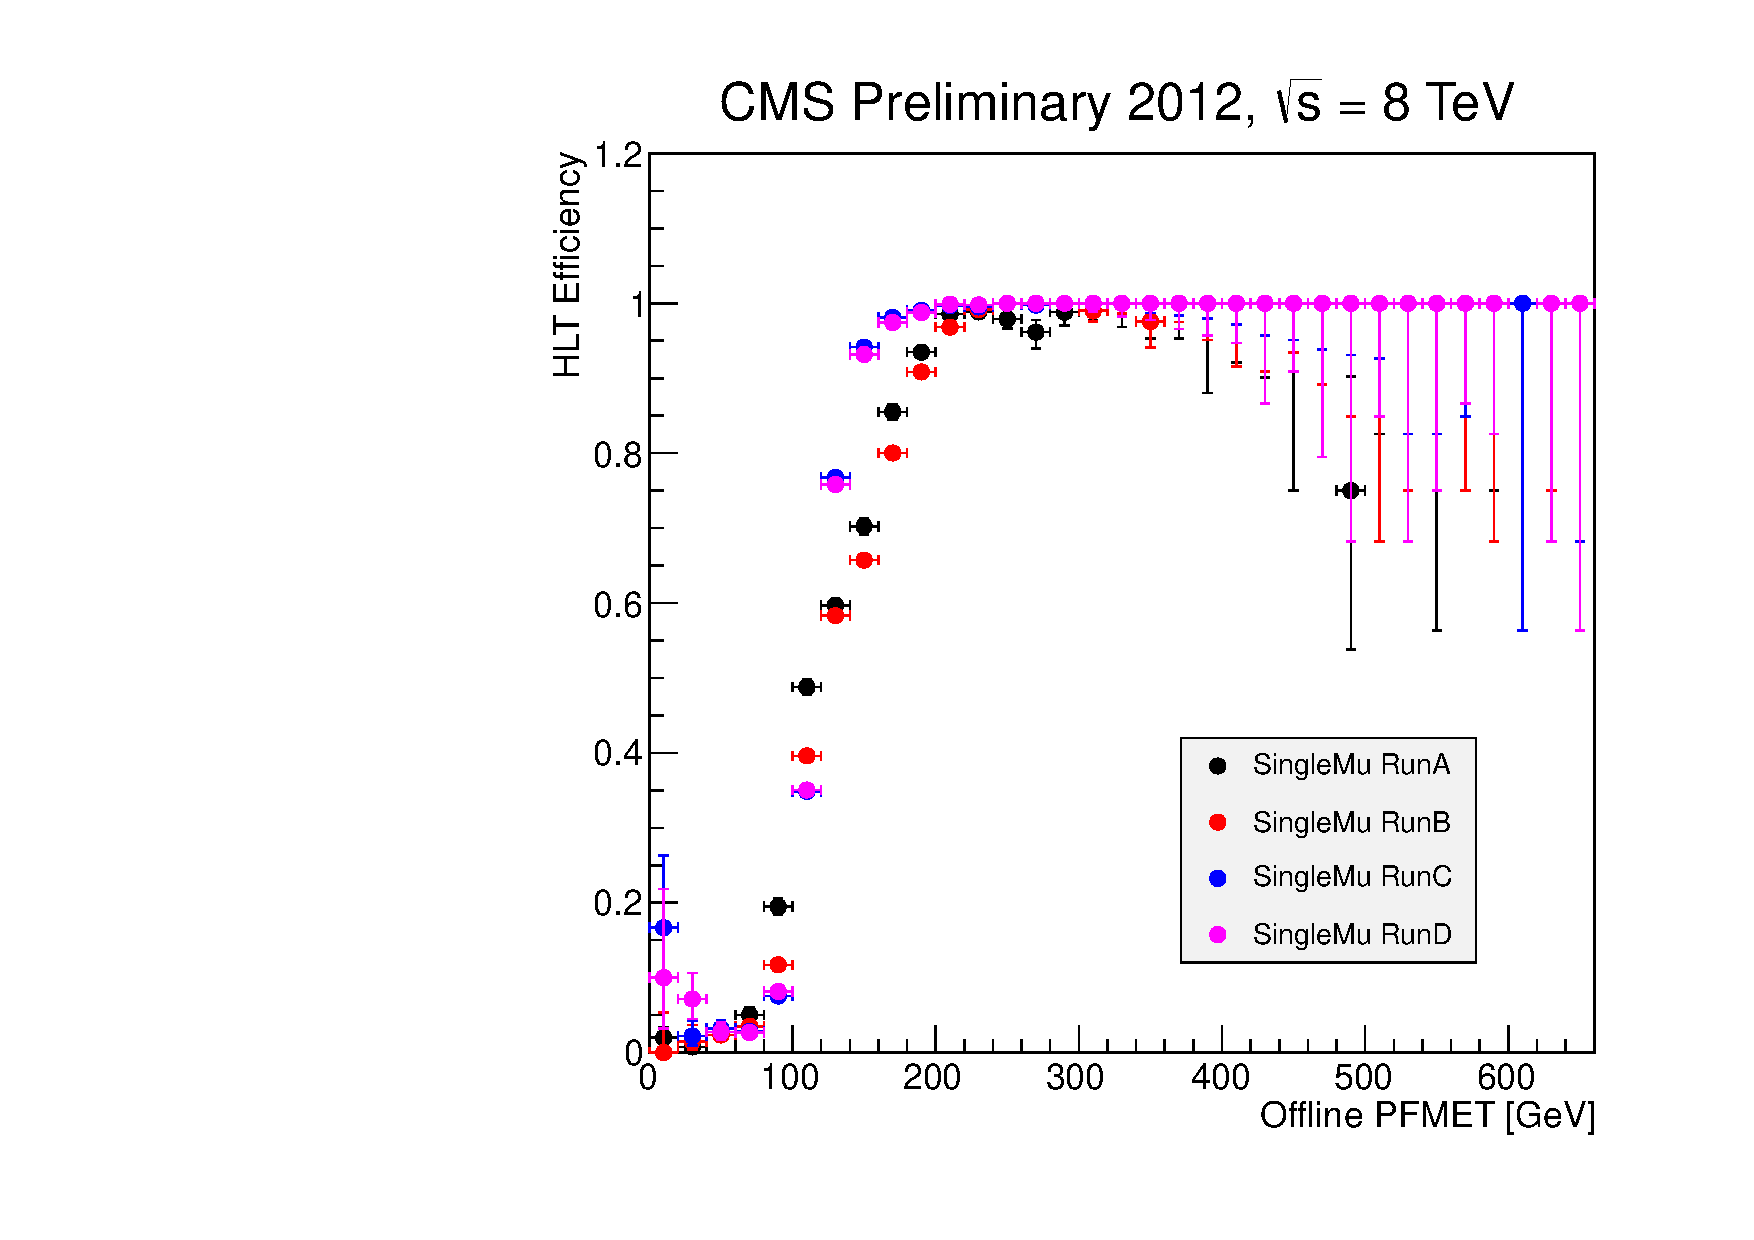
\includegraphics[scale=0.35]{Figures/sus13009/MET_OR.pdf}
 \includegraphics[scale=0.35]{Figures/sus13009/Jet1_OR.pdf}
  \caption{The trigger efficiency as a function of the \MET (left) and \pt of the leading jet (right).}
	         \label{fig:trigger-1D}
  \end{center}
\end{figure}

The specific datasets used for this analysis, along with their integrated luminosities, can be found in Table~\ref{tab:dataSets}. 
The data are from a `good-run' list of \ac{LHC} runs, in which each of the subsystems of the \ac{CMS} detector were operating well, and therefore event reconstruction was optimal.
Events were re-reconstructed using the \verb+CMSSW_5_3_9_patch3+ release of the \ac{CMS} software (CMSSW), and form a part of the legacy dataset from Run I of \ac{CMS} running. 


\begin{table} %table 2    
    \begin{center}
    \caption{Datasets used in this analysis, with a total integrated luminosity of 19.7 \fbinv.}
     \begin{tabular}{clc}\hline
Era    &       Dataset  &  Int. Lumi. [$\pbinv$]\\ \hline
2012A & /MET/Run2012A-22Jan2013-v1/AOD & 889 \\
2012B & /MET/Run2012B-22Jan2013-v1/AOD & 4429 \\
2012C & /MET/Run2012C-22Jan2013-v1/AOD & 7152 \\
2012D & /METParked/Run2012D-22Jan2013-v1/AOD & 7315 \\ \hline
                \end{tabular}
                    \label{tab:dataSets}
\end{center}
\end{table}
%The data are reconstructed with the \verb+CMSSW_5_3_2_patch4+ release. %The good-run list and luminosity have been obtained by using the JSON files listed in~\cite{bib:ANA_data_JSON}, with all subsystems marked ``GOOD''.




%
\section{Background MC simulation} 
\label{sec:GEN}
\ac{MC} simulation of \ac{SM} backgrounds are used, directly and indirectly, to estimate the contribution of \ac{SM} backgrounds to the number of events in the search regions. 
The \ac{SM} processes considered are; single top quark and top quark pair production (\ttbar), \W or \Z bosons produced in association with jets, diboson (\W\W, \W\Z, \Z\Z, \W$\gamma$ and \Z$\gamma$) production and QCD multijet processes.

The simulation of each sample follows a similar procedure.
Events are generated using a matrix element event generator such as \MADGRAPH{}~\cite{madgraph,madgraph2}, which simulates the underlying process at parton level. 
The event is then passed through a parton showering programme, usually \PYTHIA{}~\cite{pythia,pythia8,pythia-z2} in which partons undergo hadronization: quarks hadronize into jets.
It is finally passed through a simulation of the CMS detector to mimic the detector's response to the event.
All simulated \ac{SM} background events have gone through a \GEANTfour~\cite{Geant4-1,Geant4-2} simulation of the detector. 
This is a `full' simulation, computationally expensive and providing accurate responses to the simulated physics objects.  
For simulation of signal (detailed later), a `fast' simulation~\cite{FASTSIM} is used instead as it is around 100 times faster to process each event and has a comparable accuracy.

Samples of \Z bosons decaying invisibly (\znunubr{}\,+\,jets), \ttbar, and diboson events 
are simulated using \MADGRAPH{}5 interfaced with \PYTHIA{}6.4.24. 
To evaluate the content of the proton in the initial state, the CTEQ6L \ac{PDFs} are used~\cite{CTEQ6}. 
Samples are simulated using the custom CMS event tune Z2$^{*}$, which is derived from the Z1 tune~\cite{pythia-z2} which uses the CTEQ5L \ac{PDFs}, whereas the Z2$^{*}$ uses the CTEQ6L set.
Simulated \zpj{} and \wpj{} events are generated in the same way, where a cut has been placed on the transverse momentum of the boson, $\pt > 100$ \GeV, in order to increase the number of generated events that pass offline selection requirements (and where the production cross section has been modified accordingly).
QCD multijet events are generated with \PYTHIA{}6.4.24, again using tune Z2$^{*}$ and CTEQ~6L1~\ac{PDFs}. 
Single top quark processes (s-channel, t-channel and tW-channel production) are generated using \POWHEG~\cite{powheg_st,powheg_tw}.
Decays of the $\tau$ lepton are simulated using the \TAUOLA{} 27.121.5 package~\cite{TAUOLA}. 

To ensure no double counting in phase space between the underlying event and the fragmentation and hadronization process, the MLM shower matching prescription~\cite{bib:GEN_MLM} is used, in which partons from the matrix element calculation are matched to jets resulting from the hadron shower.
In order to avoid double counting photons from the \PYTHIA shower in \wpj{} and \W$\gamma$ samples (and similarly for \zpj{} and \Z$\gamma$ samples), 
events from the \wpj{} and \zpj{} simulation which have a photon from \ac{ISR} or \ac{FSR}, of $\pt(\gamma)>5$ \GeV, are removed.


\section{Object reconstruction}

In Chapter~\ref{chap:detector} the CMS detector and reconstruction methods are discussed at length, including those used in this analysis. 
Here, I briefly recap the important features of the object reconstruction and give more detail on the object definitions.

\subsection{Jets and \MET}

Jets and \MET are reconstructed using a \ac{PF}
technique~\cite{PFT-09-001}. The algorithm produces a unique list 
of particles in each event, using the combined information from all 
CMS subdetectors. This list is then used as input to the jet 
clustering, which reconstructs jets using the anti-k$_{\mathrm{T}}$
algorithm~\cite{bib:akjets} with a distance parameter of 0.5.  
The missing transverse energy vector is computed as the negative vector 
sum of the transverse momenta of all particles reconstructed in the 
event, except muons.


Jet energies are corrected to establish a uniform calorimeter 
response in $\eta$ and an absolute response in \pt calibrated at 
the particle level.  
\ac{JES} corrections are derived from simulation, and a residual correction is derived 
from the data by measuring the \pt balance in dijet events~\cite{bib:ANA_JME-10-010}.
The jet energy corrections used are `L2L3Residual' and `L1FastJet'.
To resolve any ambiguity in the reconstruction of jets and leptons, a jet is removed from the event if the energy fraction of an electron or muon in the jet is greater than 0.5.



\subsection{Leptons}

Leptons are also reconstructed using the \ac{PF} algorithm and the definitions of objects are in accordance with the \ac{CMS} recommendations.
In addition to muons, electrons and $\tau$ leptons are also used in the analysis.
Muons either pass a ``loose'' or ``tight'' selection criteria (which has more stringent requirements). 
Electrons must pass a ``loose'' selection criteria, and the \ac{HPS} algorithm with ``loose'' criteria is used to reconstruct hadronically decaying $\tau$ leptons ($\tauh$).

A loose muon must have \pt greater than 10~\GeV, and be tagged as a Global or Tracker muon -- meaning that it must
have independent tracks from both the tracker and the muon systems that join together, or that a series of hits in the tracker matches up with at least one hit in the muon system~\cite{CMS-PAPER-MUO-10-004}. 
%
A tight muon must have \pt greater than 20~\GeV and be central -- $|\eta|<2.4$. 
It must also be considered a Global muon, with additional requirements on the global muon track. 
There must be at least one hit from the muon chambers included in the global track, and the $\chi^{2}$ of the global track must be less than 10. These requirements suppress mistaken muon identification as a result of hadronic punch-through from the \ac{HCAL} and the magnet, and suppress muons originating from in-flight decays.
There must also be hits in at least two of the muon stations, which acts to reduce the number of accidental track-to-segment matches.
In order to suppress the number of cosmic muons (and further suppress muons from in-flight decays), the transverse impact parameter of the track ($d_{xy}$) as reconstructed in the tracker must be less than 2~mm from the primary vertex. 
Requiring the longitudinal impact parameter ($d_{z}$) to be less than 5~mm has a similar effect, as well as reducing the number of muons which originate from \ac{PU}.
Additional demands on the number of hits in the pixel system ($>0$) and the number of tracker layers with hits ($>5$) further suppress in-flight muon decays, and guarantee a good measurement of the muon \pt.

The electron identification used in the analysis is loose. To be classified as an electron, a track in the tracker must match up to a supercluster in the \ac{ECAL}. 
The \pt must be greater than 10~\GeV, 
and the electron reconstruction avoids the gap between the \ac{ECAL} barrel and endcap where there is no instrumentation: 
$1.44< |\eta| < 1.56 $. 
In addition, various simple parameters regarding the supercluster shower shape, matching between the \ac{ECAL} cluster and track, 
the ratio of energy deposited in the \ac{ECAL} and \ac{HCAL}, and impact parameters distinguish between primary electrons and those originating from bremsstrahlung and photon pair conversion. More information can be found in Ref.~\cite{CMS:elecReco}.

To ensure that electrons and muons are isolated -- not close to a jet or other object -- they must satisfy requirements on the isolation parameter $R$, defined as
\begin{equation}
R = \frac{\sum{\ET_{\text{charged hadrons}}}+ \sum{\ET_{\text{neutral hadrons}}}+ \sum{\ET_{\text{photons}}} }{\pt},
\end{equation} 
where the hadrons and photons are considered in a cone with radius $\sqrt{\Delta \phi ^{2} + \Delta \eta ^{2}}=0.4$ around the lepton direction.
Tight muons must have $R<0.2$, and loose electrons must have $R<0.15$.
Isolations are corrected for the effect of \ac{PU} using $\Delta\beta$ corrections~\cite{deltabeta_htautau7tev}.


The $\tau$ lepton decays hadronically 65\% of the time, with the dominant decay modes consisting of one or three charged $\pi^{\pm}$ mesons, and up to two neutral $\pi^{0}$ mesons.
The \ac{HPS} algorithm first reconstructs the $\pi^{0}$ component of the \tauh decay using a \ac{PF} anti-k$_{\rm T}$ jet with distance parameter 0.5, and then combines with charged hadrons to build a \tauh. 
`Strips' are constructed from \ac{PF} photons and electrons, starting with the most energetic electromagnetic particle within the seed jet, and combining all surrounding electromagnetic particles.
Strips with $\pt > 1$~\GeV are then combined with charged hadrons to provide a \tauh candidate. 
Here, the candidate must have $\pt > 20$~\GeV and $|\eta| < 2.3$ and the loose requirements of the algorithm are used which correspond to approximately 1\% of jets to be misidentified as a $\tauh$.
Again, $\Delta\beta$ corrections account for \ac{PU}. 
More information can be found in Ref.~\cite{bib:HPStaus}. 
%It must pass the loose combined isolation discriminant (LooseCombinedIsolationDeltaBetaCorr)
%\item pass DecayModeFinding
%\item passes AgainstElectronLoose discriminant
%\item passes AgainstMuonTight2 discriminant



\section{Event selection}
\label{sec:ANA}

The aim is to select signal candidate events while rejecting as much background as possible.
A final state with one, high \pt leading jet, and large \MET from the LSPs leaving the detector form the basis of the event selection in order to be sensitive to compressed \ac{SUSY} signatures.

\subsection{Event Cleaning}

The first stage of the event selection, after the trigger, is to reject any events that have passed the trigger due to instrumental noise or non-collision backgrounds.

Events are required to have at least one well-reconstructed primary vertex~\cite{bib:ANA_Tk}, where it is reconstructed in a 24~cm window along the beam axis, within a radius of $\rho<2$~cm orthogonal to the plane of the beam. %The number of degrees of freedom must be less than 4.
To reject events that have ``scraping'' tracks due to beam-gas interactions close to the interaction point, in events where there are 10 or more tracks at least 25\% must be good quality; that is, satisfy various requirements on the number of hits, the \pt of the track, the $\chi^{2}$ of the combination of hits which build the track etc.
To remove events with spurious \MET reconstruction, different methods of calculating the \MET are compared. The value of \MET, reconstructed using the \ac{PF} algorithm, must be comparable with the \MET calculated using calorimetric information only: events with (PF \MET - calo \MET)$ > 2 \times$ calo \MET are discarded.



%event cleaning
% The reported TOC/TEC problem \cite{bib:TOCTEC} has been shown to have a negligable effect here.
% There is a large discrepancy between PFMET and caloMET in affected events, 
% see Appendix~\ref{toctec} for comparison between PFMET and caloMET which shows no significant discrepancies between the two. 
% The requirement on PFMET and caloMET removes the majority of these events, and those remaining have been visually inspected.


Beam-halo and other beam-related backgrounds~\cite{bib:ANA_BeamHalo}, which arise when the beams interact with the beam pipes, 
can deposit energy in both the \ac{ECAL} and \ac{HCAL} leaving no associated tracks.
Cosmic muons also can give rise to fake \MET, 
or leave similarly spurious deposits - leading to fake jets - as they deposit energy in one or more of the subdetectors while leaving no tracks, or tracks which do not originate from the primary vertex.
Similarly, instrumental noise can lead to large apparent deposits in the \ac{ECAL} or \ac{HCAL}. 
Stringent requirements are therefore placed on the neutral and charged hadronic and electromagnetic content of jets:
\begin{itemize}
\item Leading jet charged electromagnetic fraction $<$ 0.7
\item Leading jet charged hadronic fraction $>$ 0.2
\item Leading jet neutral electromagnetic fraction $<$ 0.7
\item Leading jet neutral hadronic fraction $<$ 0.7
\item Second jet neutral electromagnetic fraction $<$ 0.9
\item Second jet neutral hadronic fraction $<$ 0.7
\end{itemize}
These conditions also reject high \pt photons and electrons which are misidentified as jets due to 
energy deposits in the \ac{HCAL}; the energies assigned to neutral hadrons in the 
ECAL and HCAL must sum to less than 70\% of the total jet energy.
In addition, jets are also required to pass a loose identification criterion which rejects fake jets due to calorimeter noise. 

The distributions for the neutral and charged energy fractions of the first and second jet in events (where jets are \pt ordered) before and after these set of noise cleaning cuts are applied are shown in Figures~\ref{fig:ANA_energy_fraction_cleanup} and~\ref{fig:ANA_energy_fraction_cleanup_cut}. 
They are very effective at removing noisy events, with good data/MC agreement after the cuts have been applied.

%The application of all event cleaning criteria results in the loss of 4.2\% of the events for a representative ADD signal, 1.8\% of events for a representative dark matter model and 6.7\% for a representative Unparticle signal.

\begin{figure}[!Hhtb]%[tb]
  \begin{center}
  \includegraphics[scale=0.30]     {Figures/sus13009/nocut/PFAK5JetChaEmEngFrac.pdf}
  \includegraphics[scale=0.30]     {Figures/sus13009/nocut/PFAK5JetChaHadEngFrac.pdf}
  \includegraphics[scale=0.30]     {Figures/sus13009/nocut/PFAK5JetNeuEmEngFrac.pdf}
  \includegraphics[scale=0.30]     {Figures/sus13009/nocut/PFAK5JetNeuHadEngFrac.pdf}
  \includegraphics[scale=0.30]     {Figures/sus13009/nocut/PFAK5JetNeuEmEngFrac2.pdf}
  \includegraphics[scale=0.30]     {Figures/sus13009/nocut/PFAK5JetNeuHadEngFrac2.pdf}
  \caption{Hadronic and electromagnetic energy fractions from charged 
and neutral particles, before cleanup cuts on these quantities are 
applied.  We require the charged 
hadronic fraction of the jet to be above 20\% and the neutral electromagnetic and hadronic energy fractions to be below 70\% of the total leading jet energy.
We require the neutral electromagnetic energy to be below 90\% and the neutral hadronic energy of the second jet to be below 70\% of the total second leading jet energy. }
         \label{fig:ANA_energy_fraction_cleanup}
  \end{center}
\end{figure}
%
\begin{figure}[!Hhtb]
  \begin{center}
  \includegraphics[scale=0.30]     {Figures/sus13009/cut/PFAK5JetChaEmEngFrac.pdf}
  \includegraphics[scale=0.30]     {Figures/sus13009/cut/PFAK5JetChaHadEngFrac.pdf}
  \includegraphics[scale=0.30]     {Figures/sus13009/cut/PFAK5JetNeuEmEngFrac.pdf}
  \includegraphics[scale=0.30]     {Figures/sus13009/cut/PFAK5JetNeuHadEngFrac.pdf}
  \includegraphics[scale=0.30]     {Figures/sus13009/cut/PFAK5JetNeuEmEngFrac2.pdf}
  \includegraphics[scale=0.30]     {Figures/sus13009/cut/PFAK5JetNeuHadEngFrac2.pdf}
  \caption{Hadronic and electromagnetic energy fractions from charged 
and neutral particles, after clean-up cuts on these quantities are 
applied.}
         \label{fig:ANA_energy_fraction_cleanup_cut}
  \end{center}
\end{figure}


\subsection{Signal region event selection}

Once events passing the trigger have been filtered to remove noise and fakes, 
events are selected to optimise signal acceptance while rejecting as much background as possible.

To satisfy trigger requirements, and ensure all events comfortably pass the \ac{HLT} trigger selection, 
events are required to have $\MET > 250$~\GeV and the most energetic jet ($j_1$) in the event is required 
to have $\pt(\,\mathrm{j}_1)>110~\GeV$ and $|\eta(\,\mathrm{j}_1)|<2.4$.
%§
Signal acceptance is increased by allowing events where there is a second jet originating from \ac{ISR} (or \ac{FSR}); 
however the signal also has soft final-state jets originating from the sparticle decay products.
%
To ensure that these soft final-state jets coming from charm or bottom quarks remain invisible within the event selection,
%
and a monojet signature is maintained,
the \pt threshold at which the second and third jets are counted must be high enough that
the soft-hadronic (signal) decay products 
fall below it for a good range of signal phase space 
%(and therefore remain invisible in the event selection), 
while keeping the QCD multijet background at a manageable level.
%
Figure~\ref{stopj2pT} shows the \pt distribution of charm quarks, taken from simulation, 
for a few representative mass hypotheses in the process $\ttwocc$.
%
Placing the jet counting threshold at $\pt >60$~\GeV, and requiring $|\eta| < 4.5$,
is a good compromise between signal efficiency and background rejection.
%
Events are therefore vetoed if they contain more than 2 jets,
where $\pt(\jet_{1})>110$~\GeV and $|\eta|<2.4$; $\pt(\jet_{2})>60$~\GeV and $|\eta|<4.5$; 
and the third jet is counted (and the event rejected) if it has $\pt(\jet_{3})>60$~\GeV and $|\eta|<4.5$.
A monojet-like topology in signal events is therefore maintained, 
allowing the search to be sensitive to both highly compressed spectra
and extending the scope to larger mass differences.  

\begin{figure*}%[tb]
  \begin{center}
  \includegraphics[scale=0.45]{Figures/sus13009/charmpt.pdf}
  \caption{Charm quark \pt spectra for mass splittings across the phase space range, $m_{\sTop}-m_{\chiOneZero}=10, 30, 80~\GeV$, for a top squark mass of 150~\GeV.
         \label{stopj2pT}}
  \end{center}
\end{figure*}



In order to reduce the background from \Z and \W-boson decays, events
with leptons are rejected.
Events containing a PFElectron with $\pt> 10\GeV$ and passing the WP95 selection and isolation requirements are rejected. 
Events containing a PFMuon with $\pt > 10$ \GeV and reconstructed as a Global and/or PF muon are also rejected. This follows recommendations from the 2012 Muon POG for a loose ID PF muon. 
%selection criteria listed below (except the $\eta$ cut) are rejected.


The analysis is performed in 7 inclusive regions of the leading jet $\pt$; $\pt >$ 250, 300, 350, 400, 450, 500 and 550~\GeV.
%Remaining events with an isolated track are eliminated, as they
%come primarily from $\Pgt$ decays.  To measure the isolation, a 
%hollow cone $0.02<\DR<0.3$ is defined around each track with 
%$\pt > 10\GeV$.  The scalar sum of the \pt of all tracks with 
%$\pt > 1\GeV$ inside the cone is calculated and the event is 
%vetoed if this sum is smaller than 1\% of the \pt of the original 
%track. The distribution of the track isolation ratio (TIV) is shown in Figure~\ref{fig:ANA_MuPt_and_TIV} for data, the SM backgrounds and a representative signal point for the ADD and dark matter models.

\subsection{Control region event selection}

A control sample of $\mu$+jet events is used to estimate backgrounds in a data-driven way. 
In order to get a very clean control sample muons are required to pass Tight Muon selection requirements as recommended by the Muon POG. 
In addition to kinematic and identification requirements, muon candidates are also required to be isolated using the combined relative isolation variable as defined by the Muon POG for a cone of radius 0.12.%. The relative combined isolation $R$ is defined as the sum of the \pt\ of the charged hadrons, neutral hadrons and photon contributions computed in a cone of radius 0.4 around the lepton direction, divided by the lepton \pt,
%\begin{equation}
%R_e = \frac{\Sigma_{i}[p_{Ti}({\rm chargedHadron})+ max(p_{Ti}({\rm neutralHadron})+ p_{Ti}({\rm Photon}) - EffArea*fastJetRho)]}{p_{T}}.
%\end{equation}
%\begin{equation}
%R_{\mu} = \frac{\Sigma_{i}[p_{Ti}({\rm chargedHadron})+ p_{Ti}({\rm neutralHadron})+ p_{Ti}({\rm Photon})]}{p_{T}}.
%\end{equation}
A summary of the kinematic, identification and isolation selection criteria for muons is shown below.\\ \\
%{\bf Electron Identification}
%\begin{itemize}
%\item \pt $> 20$ \GeV
%\item $|\eta|<1.44$ or $1.56<|\eta|<2.5$
%\item WP80 selection
%\item R $<$ 0.2
%\end{itemize}
{\bf Muon Identification}
\begin{itemize}
\item \pt $> 20$ \GeV
\item $|\eta|< 2.4$
\item Global and PF muon
\item $|d_{xy}| <$ 2 mm
\item $|dz| < $ 5 mm
\item $\chi^{2}$/dof $<$ 10
\item R $<$ 0.12
\item Tracks associated to muons must satisfy:
\begin{itemize}
\item at least one hit in pixel,
\item at least one muon chamber hit included in the global-muon track fit
\item segments in at least two muon stations.
\item at least 5 tracker layers with hits
\end{itemize}
\end{itemize}


\begin{figure}%[!Hhtb]
  \begin{center}
  \includegraphics[scale=0.30]     {Figures/sus13009/cut/Jet1Pt.pdf}
  \includegraphics[scale=0.30]     {Figures/sus13009/cut/Jet1Eta.pdf}
  \includegraphics[scale=0.30]     {Figures/sus13009/cut/Jet2Pt.pdf}
  \includegraphics[scale=0.30]     {Figures/sus13009/cut/Jet2Eta.pdf}
   \includegraphics[scale=0.30]     {Figures/sus13009/cut/NJet.pdf}
   \includegraphics[scale=0.30]     {Figures/sus13009/cut/dPhi_Jet1_Jet2.pdf}
   \includegraphics[scale=0.30]     {Figures/sus13009/cut/MetLep1.pdf}
   \caption{Plots of basic selection variables.  All figures except for the \pt and $\eta$ of the second leading jet are N-1 plots so all cuts are applied except the one being plotted (the leading jet $\pt$ cut for all plots except the jet $\pt$ and jet $\eta$ is set to 110 GeV). The leading SM backgrounds from \znunu\,+\,jets and \wpj events are normalised using a data-driven technique.%SM backgrounds are normalised as described in to data where available.
         \label{fig:ANA_Jet_selection_plots}}
  \end{center}
\end{figure}
%\begin{figure}[tb]
%  \begin{center}
%  \includegraphics[scale=0.35]     {cut/TIV.pdf}
%  \caption{Additional cleanup variables investigated.  We reject events with muons or electrons above 10\GeV and apply the TIV isolation as described in the text.
%         \label{fig:ANA_MuPt_and_TIV}}
%  \end{center}
%\end{figure}
A summary of all the selection criteria is given in Appendix~\ref{app:eventsel}.
Some of the kinematic distributions are shown in Figure~\ref{fig:ANA_Jet_selection_plots}.
%Fig.~\ref{fig:ANA_Jet_selection_plots} where the full monojet selection has been applied with a $\MET$ cut of 250 \GeV. All the distributions have been normalised as described in Appendix~\ref{app:normalisation}.

%The distribution of \MET for data and background after selecting monojet events and for a \MET cut of 250 \GeV is shown in Figure~\ref{fig:ANA_MET_plots}.

%We define the above described event selection with the \MET cut of 200 GeV as the baseline selection and subsequently apply tighter \MET\ selections of $\MET = 250, 300, 350, 400$ to obtain our search regions. 
%Optimisation studies have been performed for each of our signal samples to find the value of the \MET\ cut that gives the best expected limit. The study is documented in Appendix~\ref{app:opt_limit}. For both the ADD and dark matter signal points, the optimal \MET\ cut is found to be 350 \GeV. For Unparticles, the optimal \MET cut is found to be 300 \GeV or 350 \GeV, depending on the values of $d_U$. However the difference in expected limit is small and therefore a \MET\ cut of 350 \GeV is used for calculating limits, consistent with what is used for the ADD and dark matter signals.
%
%\begin{figure}[tb]
%  \begin{center}
%  \includegraphics[scale=0.45]{cut/Met.pdf}
%  \caption{The $\MET$ distribution after all selection cuts are applied for data and backgrounds.Representative signal distributions for dark matter, ADD and Unparticles are also overlaid. Events with $\MET > 1 \TeV$ are included in the overflow bin.}
%         \label{fig:ANA_MET_plots}  
%  \end{center}
%\end{figure}

Table \ref{tab:SEL_TabDataMC200} lists the number of events selected at each step of the analysis, for data and simulation.
\begin{table*}[htb] %table 7 v04 110811:05  
        \begin{center}
        \caption{Number of events selected at each step of the analysis, for data and simulation. Backgrounds are obtained from MC and normalised as described in Appendix~\ref{app:normalisation}.}%from $W$ and $Z$ use $\PYTHIA$8 with tune Z2 normalised to data, and with pile-up reweighting.} 
\label{tab:SEL_TabDataMC200}
 {\footnotesize
               \begin{tabular}{l|rrrrrrr|r} \hline
Selection     & \wpj & \zpj & \znunu\,+\,jets & Diboson &  $\ttbar$ &  Single top  &  QCD & Total BG   \\ \hline 
Cross section (pb) & 228.9  & 40.5   & 588.3  & 234.0  & 1.085e6  & 114.8  & 105.7  &   \\ \hline
%Generated events   & 1.27e7 & 2.66e6 & 1.45e7 & 6.86e6 & 4.27e7   & 7.06e6 & 2.98e7 &   \\ \hline
Trigger                        & 2514352 &  190332   & 4337526 &  65666  & 461413 & 77284 &  5429269 &  13075841 \\ 
$\MET >200$ \GeV               & 317656  &  30242    & 134578  &  9572   & 63174  & 9289  &  87605   &  652117   \\
Noise Cleaning                 & 292550  &  27880    & 123420  &  8706   & 59412  & 8525  &  81668   &  602162   \\
$\pt(\,\mathrm{j}_1)>$110~\GeV & 279323  &  26652    & 117513  &  8045   & 53353  & 7752  &  80844   &  573484   \\ 
$\njets \le 2$      	       & 254058  &  24413    & 109313  &  7287   & 29364  & 5596  &  44247   &  474278   \\ 
$\Delta\phi(j_1,j_2)<2.5$      & 237533  &  22947    & 104158  &  6984   & 25312  & 4815  &  8433    &  410181   \\ 
Muon veto                      & 106236  &  1511     & 104152  &  4051   & 9826   & 1892  &  7444    &  235112   \\ 
Electron veto                  & 79407   &  1004     & 104065  &  3459   & 6557   & 1325  &  7401    &  203218   \\ 
Tau veto                       & 71808   &  807      & 103106  &  3248   & 5599   & 1147  &  7047    &  192762   \\ \hline 
$\pt(\,\mathrm{j}_1)>$250 \GeV, 
& \multirow{2}{*}{13641}
& \multirow{2}{*}{127}   
& \multirow{2}{*}{22615}
& \multirow{2}{*}{639}
& \multirow{2}{*}{602}
& \multirow{2}{*}{172}
& \multirow{2}{*}{819}
& \multirow{2}{*}{38615}    \\
                $\MET>$250 \GeV   &        &           &          &         &         &        &           &           \\
$\pt(\,\mathrm{j}_1)>$300~\GeV   &6873    &  75       &11093     & 369     & 344     & 97     &  546      &  19397   \\ 
$\pt(\,\mathrm{j}_1)>$350~\GeV   &3182    &  40       &5231      & 206     & 178     & 49     &  332      &  9218    \\ 
$\pt(\,\mathrm{j}_1)>$400~\GeV   &1501    &  25       &2617      & 113     & 91      & 21     &  181      &  4549    \\ 
$\pt(\,\mathrm{j}_1)>$450~\GeV   &751     &  17       &1335      & 64      & 48      & 11     &  92       &  2318    \\ 
$\pt(\,\mathrm{j}_1)>$500~\GeV   &376     &  11       &727       & 36      & 27      & 5.2    &  61       &  1244    \\ 
$\pt(\,\mathrm{j}_1)>$550~\GeV   &204     &  7.4      &406       & 21      & 18      & 3.2    &  34       &  693     \\ \hline 
\end{tabular}} 
\end{center}
\end{table*}



\section{Data driven background estimation}
\label{sec:BKG}

The dominant backgrounds remaining after the monojet event selection are electroweak backgrounds from ``invisible $Z$'' decays and W\,+\,jets.
Both of these backgrounds are estimated from data by selecting a control sample of $\mu$+jet events, where \zmumu\,+\,jets is used to predict the invisible Z background and \wmunu\,+\,jets is used to predict the remaining W\,+\,jets background.
This muon control sample is derived from the same dataset as the signal.

The control samples are obtained by applying the full monojet selection with the exception of the lepton veto.
%Well-reconstructed 
%and isolated muons with $\pt(\mu)>20\GeV$  are selected following 
%the criteria described in Section~\ref{sec:ANA}.
To obtain a sample of \zmumu\ events, one well identified and isolated muon satisfying the selection in Section~\ref{sec:ANA} is required and the invariant mass of this muon with another reconstructed muon in the event is required to be between 60 and 120 GeV. 
%Compared to the previous version of the analysis, where the second muon was also required to be isolated and well identified, we  an increase of 20$\%$ in the statistics of the \zmumu\ sample.
A sample of \wmunu\,+\,jets is similarly obtained by requiring one well identified and isolated muon and with a reconstructed W transverse mass between 50 and 100 GeV.

Tables~\ref{tab:Zmuontable} and~\ref{tab:Wmuontable} show the event yields obtained for the \zmumu\ and \wmunu\ control samples and the predicted backgrounds from MC.

\begin{table*}[!Hhtb]  %table 8   110811:05  
        \begin{center}
\caption{Event yields for the \zmumu data control samples and the backgrounds from MC.
50\% uncertainty is assigned to each background (i.e. from \ttbar, single top, and diboson events) and these are combined in quadrature to get the total uncertainty on 
the number of background events in the \zmumu sample.}
\label{tab:Zmuontable}
{\small
                \begin{tabular}{l|ccccccc|cc} \hline
                          &\zpj & \wpj & \znunu\,+\,jets & \ttbar  & Single t & QCD    & Diboson &  All MC & Data\\\hline
%numbers on 1 Oct: new ntuple
$\pt(\,\mathrm{j}_1)>$250~\GeV  & 3067 & 0 &  0 & 37  & 5.7 & 0 & 68  & 3177 &  2547 \\
$\pt(\,\mathrm{j}_1)>$300~\GeV  & 1577 & 0 &  0 & 21  & 2.2 & 0 & 41  & 1641 &  1235 \\
$\pt(\,\mathrm{j}_1)>$350~\GeV  & 757  & 0 &  0 & 9.9 & 0.9 & 0 & 24  & 791  &   567 \\  
$\pt(\,\mathrm{j}_1)>$400~\GeV  & 382  & 0 &  0 & 4.8 & 0.9 & 0 & 13  & 401  &   277 \\
$\pt(\,\mathrm{j}_1)>$450~\GeV  & 198  & 0 &  0 & 0.7 & 0   & 0 & 8.2 & 207  &   150 \\
$\pt(\,\mathrm{j}_1)>$500~\GeV  & 109  & 0 &  0 & 0   & 0   & 0 & 4.4 & 113  &   79  \\ 
$\pt(\,\mathrm{j}_1)>$550~\GeV  & 62   & 0 &  0 & 0   & 0   & 0 & 2.6 & 65   &   40  \\ \hline
                 \end{tabular}}                                                                                   
\end{center}
\end{table*}



\begin{table*}[!Hhtb]
        \begin{center}
\caption{Event yields for the $W \rightarrow \mu \nu$ data control samples and the backgrounds from MC.
50\% uncertainty is assigned to each background (i.e. from $\Z$\,+\,jets, \ttbar, single top, QCD and diboson events) and these are combined in quadrature to get the total uncertainty 
on the number of background events in the $W \rightarrow \mu \nu$ sample.}
\label{tab:Wmuontable}
 {\small
  \begin{tabular}{l|ccccccc|cc} \hline
                         &\zpj & \wpj & \znunu\,+\,jets & \ttbar  & Single t & QCD  & Diboson  & All MC & Data\\\hline
%numbers 1July
$\pt(\,\mathrm{j}_1)>$250~\GeV  & 11436 & 183 & 0 & 608 & 158 & 0.3 & 197 & 12582  & 11371\\
$\pt(\,\mathrm{j}_1)>$300~\GeV  & 5712  & 94  & 0 & 313 & 80  & 0.3 & 121 & 6320   & 5477 \\
$\pt(\,\mathrm{j}_1)>$350~\GeV  & 2694  & 44  & 0 & 151 & 41  & 0.3 & 71  & 3001   & 2547 \\
$\pt(\,\mathrm{j}_1)>$400~\GeV  & 1349  & 22  & 0 & 76  & 22  & 0.3 & 41  & 1509   & 1258 \\
$\pt(\,\mathrm{j}_1)>$450~\GeV  & 712   & 9.9 & 0 & 41  & 13  & 0.3 & 22  & 798    & 668  \\
$\pt(\,\mathrm{j}_1)>$500~\GeV  & 389   & 6.6 & 0 & 20  & 7.8 & 0.3 & 13  & 437    & 352  \\
$\pt(\,\mathrm{j}_1)>$550~\GeV  & 223   & 3.7 & 0 & 11  & 4.8 & 0.3 & 6.5 & 249    & 184  \\ \hline 
                \end{tabular}}                                                              \end{center}
\end{table*}
A comparison between data and MC for the dimuon invariant mass and momentum after all the selection cuts and a \pt(j1) cut of 250 \GeV is shown in Figure~\ref{fig:BKGR_Z_mass}.%, where the missing transverse energy is redefined as the vector sum of the muon transverse momentum and missing transverse energy to emulate the missing energy in events where the lepton is lost.
\begin{figure}[!Hhtb]
  \begin{center}
  \includegraphics[scale=0.39]{Figures/sus13009/cut/ZleplepMT_60_120.pdf}
  \includegraphics[scale=0.39]{Figures/sus13009/cut/ZleplepPT_60_120.pdf}
  \caption{Invariant mass and transverse momentum of the dimuon pair in the \zmumu control sample.}
  \label{fig:BKGR_Z_mass}
  \end{center}
\end{figure}

A comparison between data and MC for the transverse mass and momentum of the W after the full selection and for $\pt(\,\mathrm{j}_1) > 250 \GeV$ is shown in Figure~\ref{fig:BKGR_W_mass}.%, where the missing transverse energy is defined as the vector sum of the muon transverse momentum and missing transverse energy to emulate the missing energy in events where the lepton is lost.

\begin{figure}[!Hhtb]
  \begin{center}
  %\includegraphics[scale=0.39]{cut/WlepnuMT_50_100.pdf}
  \includegraphics[scale=0.39]{Figures/sus13009/cut/WlepnuMT.pdf}
  \includegraphics[scale=0.39]{Figures/sus13009/cut/WlepnuPT2_50_100.pdf}
  \caption{Transverse mass $M_{T}$ of the muon (left) and transverse momentum of $W^\pm$ candidates in the W mass window, $50 - 100 \GeV$ in the $W \rightarrow \mu \nu$ sample.}
  \label{fig:BKGR_W_mass}
  \end{center}
\end{figure}

\subsection{Estimation of \znunu background}

The \zmumu and \znunu events share similar kinematic characteristics and by interpreting the pair of muons as missing energy, the topology of the process in which the $Z$ boson decays to neutrinos can be reproduced.  The missing transverse energy in the \zmumu event is defined as the vector sum of the transverse momentum of the muons and the \MET. The number of \znunu events can then be predicted using:

\begin{equation}
N(Z\rightarrow\nu\nu) = \frac{N_{obs} - N_{bgd}}{A*\epsilon}\cdot R 
\end{equation}

where $N_{\rm obs}$ is the number of observed dimuon events, $N_{\rm bgd}$ is the number of background events contributing to the dimuon sample, $A$ is the fiducial and kinematic acceptance of the detector and the efficiency of the $Z$ mass window cut, $\epsilon$ is the selection efficiency of the event and $R$ is the ratio of branching fractions for the $Z$ decay to neutrinos and a pair of muons. These factors are determined as follows:
\begin{itemize}

\item $N_{bgd}$ : The dimuon sample comprises predominantly of \zmumu events with less than 1$\%$ contamination from background. The backgrounds are taken from Monte Carlo and a 50\% uncertainty is assigned to the number. 

\item $A$ : The acceptance $A$ is defined as the fraction of all generated events where the muons are reconstructed with $\pt > 20$ \GeV and $|\eta| < 2.1$ and the invariant mass of the muons is within 60 \GeV and 120 \GeV. This is obtained from Z\,+\,jets MC using generator level information.

\item $\epsilon$ : The event selection efficiency $\epsilon$ is defined as the efficiency of reconstructing muons passing all the identification and isolation criteria and with a reconstructed invariant mass between 60 and 120 $\GeV$, given that they are within the detector acceptance. 
The efficiency is taken from MC.
It is corrected by a scale factor to account for the difference in selection efficiency between data and MC.

\item $R$ : The ratio of the branching fraction $R = (\frac{BF(\znunubr)}{BF(\zmumubr)})$ is obtained from \cite{bib:BKG_PDG} and 
   is $5.942\pm 0.019$ when $l=\mu$. 
\end{itemize}
 
The selection of \zmumu events relies upon counting the number of events at each $\pt(\,\mathrm{j}_1)$ cut, which is correlated to the PF METnoMu.
We interpret the muons as missing energy, and add their $\pt$ into the PF MET in the redefinition of the \MET.
The momentum is balanced by $\pt(\,\mathrm{j}_1)$.
This exploits the similar kinematics of \znunu and \zmumu events, treating the muons as neutrinos. 
The estimate of METnoMu and $\pt(\,\mathrm{j}_1)$ therefore relies upon successfully identifying both muons in the muonic Z decay, 
in order to add them into the \MET and imitate an invisible Z decay where of course both neutrinos contribute to the \MET and so $\pt(\,\mathrm{j}_1)$. 

If either (or both) muons in a \zmumu decay is not properly identified, 
for example the muon does not pass identification requirements but the track is reconstructed, 
the energy of the muon will be included within the PF MET calculation and our procedure does not remove it. 
This event is likely to fail a METnoMu or $\pt(\,\mathrm{j}_1)$ cut.
It will not contribute to the total number of \zmumu events and therefore reduce the total \znunu estimation.
However, if it had of been a \znunu event, 
both neutrinos would lead to genuine missing energy and so in missing such events we have under-estimated the \znunu background.

In order to correct for this effect we count the number of events in MC where METnoMu /\pt gen Z $< 0.7$ in each inclusive $\pt(\,\mathrm{j}_1)$ bin. 
A threshold value of 0.7 is chosen as the Z resolution is $\sim 0.3$ and we wish to count events in the tail of the Z mass spectrum.
This gives an estimate of the number of events where we have not properly measured or identified one or two of the muons. 
The ratio, typically $<5\%$, is calculated in each $\pt(\,\mathrm{j}_1)$ bin and combined with the difference in efficiency for a TL or TT muon selection.
A correction factor dependent on the signal region of order 5\% is therefore applied.

%In addition, a 4.7$\%$ correction is applied to the predicted \znunu background to account for an inefficiency in \zmumu\ events where the muon track is reconstructed but the muon is not identified. These events were studied by plotting the ratio of \MET and the generated $Z$ boson \pt, they are present in the low tail of the distribution, below around 0.7, in \zmumu\ events but absent in the same distribution for \znunu events. 
%We therefore estimate the selection efficiency using Z\,+\,jets MC and assign a systematic of 2$\%$ to cover the variation of the data-MC scale factor from 1.0, measured in~\cite{bib:AN-11-240}.

A correction factor is also applied to R, to account for contamination from $g^{*}$. 
   $\alpha$ is the fraction of $g^{*}$ component in the Z, found from the difference in normalised \zmumu and \znunu samples in the Z mass window.
   $\beta$ is the fraction of events lying outside the Z mass window in \znunu MC.
   The $g^{*}$ contamination can be estimated using
   \begin{equation}
    g^{*} fraction = \frac{1-\alpha}{1-\beta} 
   \end{equation}
Normalised across all $\pt(\,\mathrm{j}_1)$ bins, we find a correction factor of 1.017.


Table~\ref{tab:Zinv_factors} shows the observed \zmumu event yields and the correction factors for various \MET\ cuts. Also shown is the estimated \znunu background and the total uncertainty on it. 
%A summary of the fractional contributions of the uncertainties to the total error on the \znunu background is shown in Table~\ref{tab:Z_jets_sys}. 
%The dominant contribution to the uncertainty is the statistical uncertainty from the size of the \zmumu sample. 

%For the baseline selection, this is found to be 14131.5$\pm$xxxxx. This can be compared to the prediction from the invisible Z MC, 14728.9$\pm$xxxx.

\begin{table*}%[!Hhtb]  %table 8   110811:05  
        \begin{center}
\caption{Summary of the \zmumu event yields and the efficiency factors used to predict the \znunu\,+\,jets background.}
\label{tab:Zinv_factors}
\small
       \begin{tabular}{l|ccccccc} \hline
%& & & & \MET\ cut&  & &  \\
$\pt(\,\mathrm{j}_1)$ (\GeV) & $>$ 250 & $>$ 300 & $>$ 350 & $>$ 400& $>$ 450  & $>$ 500 & $>$ 550 \\ \hline 
N$_{obs}$ & 2547 &  1235 &  567&  277 & 150 & 79  & 40  \\ 
N$_{bgd}$ & 111  &  64   &  35 &  19  & 8.9 & 4.4 & 2.7 \\ 
Acceptance $A$        & 0.805  & 0.833  & 0.851  & 0.864  & 0.881  & 0.905  & 0.896  \\
Efficiency $\epsilon$ & 0.862  & 0.843  & 0.822  & 0.802  & 0.775  & 0.751  & 0.754  \\
%R &         5.942 & 5.942 & 5.942 & 5.942 & 5.942 & 5.942 & 5.942  \\ 
g* corr. factor & 1.017 & 1.017 & 1.017 & 1.017 & 1.017 & 1.017 & 1.017\\ 
\hline
\znunu &21209$\pm$1115  &10077$\pm$592 &  4597$\pm$324 & 2250$\pm$197 & 1250$\pm$137 & 663$\pm$94 & 334$\pm$65 \\ \hline
       \end{tabular}                                                                                   
\end{center}
\end{table*}


\begin{table*}%[!Hhtb]  %table 8   110811:05  
        \begin{center}
\caption{Summary of the contributions to the total uncertainty on \znunu\,+\,jets background from the various factors used in the data-driven estimation.}
\label{tab:Z_jets_sys}
                \begin{tabular}{l|ccccccc} \hline
$\pt(\,\mathrm{j}_1)$ (\GeV) & $>$ 250 & $>$ 300 & $>$ 350 & $>$ 400& $>$ 450  & $>$ 500 & $>$ 550 \\ \hline 
Statistics (N$^{obs}$)  & 2.1 &  3.0 &  4.5 &  6.5 &  8.7 &  12  &  17 \\
Background (N$^{bgd}$)  & 1.6 &  2.0 &  2.4 &  2.7 &  2.9 &  2.9 &  3.5\\ 
Acceptance              & 2.0 &  2.1 &  2.1 &  2.2 &  2.4 &  2.5 &  2.9\\
Efficiency              & 2.1 &  2.1 &  2.3 &  2.6 &  3.3 &  4.4 &  5.5\\
R                       & 2.0 &  2.0 &  2.0 &  2.0 &  2.0 &  2.0 &  2.0\\ \hline
Total                   & 5.3 &  5.9 &  7.0 &  8.8 &  11  &  14  &  19 \\  \hline 
\end{tabular}
\end{center}
\end{table*}


\subsection{Estimation of W\,+\,jets background}
The second most dominant background arises from W+jet events that are not removed by the explicit lepton veto cut. These can come from hadronically decaying taus or events in which the lepton (electron or muon) is not identified, not isolated or not within the acceptance region. 
Such events in which the electron, muon or hadronic tau are effectively `lost' are estimated by using the $W \rightarrow \mu\nu +$jets control sample. The \wmunu events are first corrected for the acceptance ($A'$) and efficiency of reconstructing the events ($\epsilon'$) in the detector to obtain the total number of generated events ($N_{tot}^{\mu}$). 
\begin{equation}
N_{tot}^{\mu} = \frac{N_{obs} - N_{bgd}}{A'\epsilon'} \label{eqn:Ntot}
\end{equation}

This is subsequently weighted by the inefficiency factors (detailed below) to obtain the predicted number of events that would not be rejected by the lepton veto and thus remain in the monojet sample.

The total number of $W \rightarrow \mu\nu +$jets events that are out of the acceptance and not identified/isolated can be written as:
\begin{equation}
N_{lost \mu} = N_{tot}^{\mu}*(1 - A_{\mu}\epsilon_{\mu}).
\end{equation}
%\begin{eqnarray}
%N_{!A}^{\mu} &=& N_{tot}^{\mu}*(1 - A_{\mu})\\
%N_{!\epsilon}^{\mu} &=& N_{tot}^{\mu}*A_{\mu}*(1 - \epsilon_{\mu})\\
%\end{eqnarray}
where $A_{\mu}$ is the acceptance and $\epsilon_{\mu}$ is the efficiency of the muon selection used in the lepton veto definition.

Similarly, for an estimation of the `lost' electron background, we start with $N_{tot}^{\mu}$ and multiply by the ratio of the 
$W \rightarrow \mu\nu +$jets and $W \rightarrow e \nu +$jets events that are predicted at the generator level in MC ($f_e$) 
to obtain $N_{tot}$ for electrons. The lost electron background is given by:
\begin{eqnarray}
N_{tot}^{e}&=& N_{tot}^{\mu}*f_e,\,\,\, {\rm where }\,\, f_{e} = \frac{N_{gen}^{e}}{N_{gen}^{\mu}}\\
N_{lost e} &=& N_{tot}^{e}*(1 - A_{e}\epsilon_{e})\\
\end{eqnarray}
where $A_{e}$ is the acceptance and $\epsilon_{e}$ is the efficiency of the electron selection used in the lepton veto definition.
The electron acceptance is obtained using generator level MC and the selection efficiency is also obtained from MC with an assumed data/MC scale factor of 1.0.% with an assigned systematic that covers the variation in efficiency between data and MC.
%Table~\ref{tab:wjetslost} summarises the estimated lost muon and electron background.
%A detailed table showing the various factors that are used to estimate this background is shown in Table~\ref{tab:wjets-summary}.

%The same procedure as that outlined in the above equations is then followed to obtain the number of events where the electron is not reconstructed/isolated or out of the acceptance. The electron acceptance is obtained using generator level MC and the selection efficiency is also obtained from MC with an assigned systematic that covers the variation in efficiency between data and MC.
%~\cite{bib:AN-11-240}.
The component of the \wpj background from hadronic tau events is estimated in the same way. The ratio of the generated \wmunu and hadronic tau events ($f_{\tau}$) is taken from MC and used to obtain $N_{tot}$ for tau events. This is subsequently weighted by the inefficiency of the tau selection used in the veto to obtain the 'lost' hadronic tau background.
\begin{eqnarray}
N_{tot}^{\tau}&=& N_{tot}^{\mu}*f_{\tau},\,\,\, {\rm where }\,\, f_{\tau} = \frac{N_{gen}^{\tau}}{N_{gen}^{\mu}}\\
N_{lost \tau} &=& N_{tot}^{\tau}*(1 - A_{\tau}\epsilon_{\tau})\\
\end{eqnarray}
The tau ID efficiency is estimated from MC with a data/MC scale factor of 1.0 and assigned an uncertainty of 6$\%$ as recommended by the Tau POG. 
The electron and muon discriminants in the Tau ID selection can also result in the Tau veto rejecting electron and muon events. The probability of an electron or muon to fake a tau is estimated from the W\,+\,jets MC and found to be negligible (below 0.1$\%$).
% No correction is made to these fake rates to account for data/MC differences as recommended by the Tau POG.  The Tau POG recommends an uncertainty of 5$\%$ on the electron fake rate for electrons in the Barrel and 10$\%$ for those in the Endcap and a 30$\%$ uncertainty on the muon fake rate. Since the fake rates are very small for our analysis, we assign 10$\%$ to electrons in both the Barrel and Endcap and the recommended 30$\%$ for muons. 
% Table~\ref{tab:wjetstau-summary} shows the tau acceptance and efficiency that are used to obtain the remaining tau hadronic background. More details on the tau acceptance, efficiency and fake rates at different stages of the monojet selection are given in Table~\ref{tab:wjets-hadronictau}. 

All of the above components can be summarised in a Master Equation for estimating the 'Lost' W background:
\begin{equation}
N_{lost} = \frac{N_{obs} - N_{bgd}}{A'\epsilon'}*\Big[(1 - A_{\mu}\epsilon_{\mu}) + f_{e}*(1 - A_{e}\epsilon_{e}) + f_{\tau}(1 - A_{\tau}\epsilon_{\tau})\Big]
\end{equation}

The factors in this equation used to estimate the lost muon, electron and hadronic tau backgrounds are detailed in Table~\ref{tab:wjetslost}.  A summary of the estimated remaining W+jet events in the monojet sample is shown in Table~\ref{tab:wjetstotal}.  


%The remaining component of the W\,+\,jets background which is not accounted for by this method is that from hadronically decaying tau. This is taken from W\,+\,jets MC and corrected by the data/MC scale factor obtained from \wmunu\ events.
%Since the control sample for this background estimation is obtained by relaxing the track isolation veto, we estimate the TIV efficiency from MC for all the \MET\ regions and apply this efficiency to obtain the final W\,+\,jets prediction. 


\begin{table*}%[!Hhtb]  %table 8   110811:05  

        \begin{center}
\caption{Estimation of the remaining W\,+\,jets background from the lost electron, muon and hadronic tau contributions.}
\label{tab:wjetslost}
 \begin{tabular}{l|ccccccc} \hline
% & & & Met cut&  & & & \\
$\pt(\,\mathrm{j}_1)$ (\GeV) & $>$250 &$>$300 & $>$350 & $>$400& $>$450  & $>$500 & $>$550 \\ \hline 
N$_{obs}$  & 11371 &  5477 & 2547 & 1258 & 668 &  352 &  184 \\
N$_{bgd}$  & 1146  &  608  & 307  & 160  & 86  &  48  &  26  \\
A'$\epsilon'$   & 0.345 &  0.345 &  0.341 & 0.346 &  0.349 &  0.361 &  0.371 \\
N$_{tot}^{\mu}$ & 29666 &  14125 &  6573  & 3176  &  1666  &  841   &  425   \\ \hline
  
Lost Muon & & & & & & & \\
A$_{\mu}\epsilon_{\mu}$ & 0.887 &   0.895 &   0.901 &   0.908 &   0.908&    0.906 &   0.907  \\
N$_{lost \mu}$          & 3350  &   1484  &   649   &   292   &   152  &    79    &   40     \\ \hline

Lost Electron & & & & & & & \\
A$_{e}$$\epsilon_{e}$ &0.615 &  0.684 &  0.734 &  0.771 &  0.793 &  0.815 &  0.823\\
f$_{e}$               &0.374 &  0.465 &  0.548 &  0.610 &  0.653 &  0.706 &  0.727\\
N$_{lost e}$          &4273  &  2077  &  958   &  444   &  225   &  110   &  55   \\ \hline

Lost Tau & & & & & & & \\
A$_{\tau}$$\epsilon_{\tau}$ & 0.253  & 0.284  & 0.298  & 0.296  & 0.294  & 0.341  & 0.325 \\
f$_\tau$                    & 0.212  & 0.235  & 0.235  & 0.228  & 0.212  & 0.201  & 0.195 \\
N$_{lost \tau}$             & 4704   & 2377   & 1083   & 510    & 249    & 112    & 56    \\ \hline


N$_{lost}$ & 12328$\pm$707 &  5939$\pm$366 & 2690$\pm$180 & 1246$\pm$92 &  627$\pm$52 & 301$\pm$29 & 150$\pm$18 \\ \hline

       \end{tabular}                                                                                   
\end{center}
\end{table*}

\begin{table*}[!Hhtb]  %table 8   110811:05  

        \begin{center}
\caption{Summary of the estimated total remaining W\,+\,jets background.}% and its comparison with the MC prediction.}
\label{tab:wjetstotal}
\small
 \begin{tabular}{l|rrrrrrr} \hline
% & & & Met cut&  & & & \\
$\pt(\,\mathrm{j}_1)$ (\GeV)  & $>$250 &$>$300 & $>$350 & $>$400& $>$450  & $>$500 & $>$550 \\ \hline 
N$_{tot}^{\mu}$     & 29666  &  14125  &  6573  & 3176   &  1666  &  841   &  425   \\ 
N$_{lost \mu}$      &  3350  &   1484  &   649  &  292   &   152  &   79   &   40   \\ 
N$_{lost e}$        &  4273  &   2077  &   958  &  444   &   225  &  110   &   55   \\ 
N$_{lost \tau}$     &  4704  &   2377  &  1083  &  510   &   249  &  112   &   56   \\ 
N$_{lost}$          & 12328$\pm$707 &  5939$\pm$366 & 2690$\pm$180 & 1246$\pm$92 &  627$\pm$52 & 301$\pm$29 & 150$\pm$18 \\ \hline
\end{tabular}
\end{center}
\end{table*}


The uncertainty on the W\,+\,jets estimation includes; the statistical uncertainty on the number of single-muon events in the data, a 50$\%$ uncertainty on the background events obtained from MC, an uncertainty on acceptance from PDFs (2\%) and MC statistics and an uncertainty on the selection efficiency $\epsilon$ from the variation in the data/MC scale factor and MC statistics. A summary of the fractional contributions of these uncertainties to the total error on the W\,+\,jets background is shown in Table~\ref{tab:wjetssys}. 
It is dominated by statistical uncertainty on $N_{obs}$ and 50\% uncertainties assigned to $N_{bkg}$.

\begin{table*}
        \begin{center}
\caption{Summary of the contributions (in \%) to the total uncertainty on the W\,+\,jets background from the various factors used in the data-driven estimation.}
\label{tab:wjetssys}
                \begin{tabular}{l|ccccccc} \hline
$\pt(\,\mathrm{j}_1)$ (\GeV)  & $>$250 &$>$300 & $>$350 & $>$400& $>$450  & $>$500 & $>$550 \\ \hline 
Statistics (N$_{obs}$) & 1.0 & 1.5 & 2.3 & 3.2 & 4.4 & 6.2 & 8.6  \\  
Background (N$_{bgd}$) & 3.3 & 3.7 & 4.0 & 4.2 & 4.2 & 4.3 & 4.4  \\ 
$A'$                   & 2.0 & 2.0 & 2.0 & 2.0 & 2.0 & 2.1 & 2.1  \\ 
$\epsilon'$            & 2.0 & 2.1 & 2.2 & 2.4 & 2.7 & 3.1 & 3.7  \\ 
$A_{\mu}$              & 0.1 & 0.1 & 0.2 & 0.2 & 0.3 & 0.4 & 0.5  \\ 
$\epsilon_{\mu}$       & 0.1 & 0.1 & 0.2 & 0.2 & 0.3 & 0.4 & 0.6  \\ 
$A_{e}$                & 0.7 & 0.9 & 1.0 & 1.1 & 1.2 & 1.3 & 1.3  \\ 
$\epsilon_{e}$         & 0.7 & 0.9 & 1.0 & 1.1 & 1.2 & 1.3 & 1.4  \\ 
$A_{\tau}$             & 0.2 & 0.2 & 0.2 & 0.2 & 0.2 & 0.3 & 0.3  \\ 
$\epsilon_{\tau}$      & 0.2 & 0.2 & 0.2 & 0.2 & 0.2 & 0.3 & 0.3  \\  \hline
Total                  & 5.7 & 6.2 & 6.7 & 7.4 & 8.2 & 9.7 & 12   \\  \hline 
\end{tabular}                                                                             
\end{center}
\end{table*}

%A summary of the fractional contributions of these uncertainties to the total error on the W\,+\,jets background is shown in Table~\ref{tab:W_jets_sys}.

%\begin{table*}%[!Hhtb]  %table 8   110811:05  
%        \begin{center}
%\caption{Summary of the contributions to the total uncertainty on W\,+\,jets background from the various factors used in the data-driven estimation.}
%\label{tab:W_jets_sys}
%                \begin{tabular}{l|ccccccc} \hline
% & & & & \MET cut & & & \\
%Source of Uncertainty  & 250 &300 & 350 & 400& 450  & 500 & 550 \\ \hline 
%Source of Uncertainty                          & $\MET > 250$ &$\MET > 300$ &$\MET > 350$ &$\MET > 400$ &   $\MET > 450$ & $\MET > 500$ & $\MET > 550$ \\ \hline 
%Statistics (N$_{obs}$) & 0.9 & 1.4 & 2.0 & 4.1 & 5.7 & 7.8 \\
%Background (N$_{bgd}$) & 7.8 & 6.8 & 5.7 & 5.8 & 5.8 & 5.4 & 7.3 \\
%Acceptance (A') & 2.0& 2.0 & 2.0 & 2.1 & 2.1 & 2.2 &  2.3 \\
%Selection efficiency ($\epsilon'$) & 2.1 & 2.2 & 2.5 & 2.9 & 3.6 & 4.6 & 5.9 \\
%Total & 
%        \end{tabular}                                                                                   
%\end{center}
%\end{table*}

\subsection{QCD Background Estimation}
\label{section:QCD}
The QCD background is predicted using MC, with a scale factor derived from a QCD rich control region.
The standard monojet event selection is applied to events, apart from those cuts which remove the majority of the QCD: $\Delta \phi(\,\mathrm{j}_1, \,\mathrm{j}_2)<2.5$ and $N_{jets} < 3$.
The $\pt$ requirement used to count jets is varied between 20 and 80 \GeV. 

\begin{figure}[htbp!]
\begin{center}
 \includegraphics[scale=0.4]{Figures/sus13009/dPhi_MetLep_Jet2.pdf}
\caption{The QCD rich region dominated by back to back jets, $\Delta \phi(\,\mathrm{\MET}, \,\mathrm{j}_2)<0.3$, shown for a jet counting cut of 60~\GeV for $\pt(\,\mathrm{j}_1) > 250 \GeV$..}
\label{dphi_METj2}
\end{center}
\end{figure}


The control region $\Delta \phi (\MET, j_{2}) < 0.3$ is selected as this is within the signal region.
Figure~\ref{dphi_METj2} shows a comparison of the data and MC for  $\Delta \phi (\MET, j_{2})$. 
%Data and background events in the QCD rich region $\Delta \phi(j1, j2)>3$ were compared; see Figure~\ref{dphi_j1j2}. 
The event yields for data and MC in this region are shown in Table~\ref{QCDtable} for each jet counting \pt threshold and for $\pt(j_{1})>250 \GeV$. 
A scale factor on the QCD background is derived using the Equation~\ref{qcdSF}. Here, 'other backgrounds' are the sum of \znunu\,+\,jets,
W\,+\,jets (corrected for the data driven estimate), \ttbar, diboson, $\Z \rightarrow \ell\ell$\,+\,jets and single top.
The uncertainty on this scale factor is due to 50\% uncertainty on each of the 'other backgrounds' and the statistical uncertainty on number of events.

\begin{equation}
\label{qcdSF}
 QCD_{s.f.} = \frac{\text{Data} - \text{Other backgrounds}}{\text{QCD MC}}
\end{equation}

Averaging across jet counting thresholds, the scale factor at each inclusive $\pt(\,\mathrm{j}_1)$ bin is found with associated error.
Scale factors for each $\pt(\,\mathrm{j}_1)$ bin are shown in Table~\ref{QCDFinaltable}.
These are applied to the final QCD estimation, and error is combined with 50\% uncertainty assigned to the QCD background from MC.
A more detailed description of this study, including the breakdown of individual backgrounds can be found in Appendix~\ref{QCDestimate}.
We find a correction factor of 1.53 at $\pt(\,\mathrm{j}_1) > 250 \GeV$ is required, decreasing to 1.35 at $\pt(\,\mathrm{j}_1) > 550 \GeV$. 
This is greater than the factor from the dijet resonance analysis of 1.24, but this is a different region of phase space so it is not unexpected.
More detail on the QCD estimation can be found in Appendix~\ref{QCDestimate}.

\begin{table}[htdp]
\caption{Event yields from MC and data at $\pt(\,\mathrm{j}_1)>250$\GeV for different values of the $\pt$ threshold used for jet counting in the QCD rich region $\Delta \phi (\MET, j_{2}) < 0.3 $. Relative uncertainty on a scale factor derived from the data is also shown.
}
\begin{center}
\begin{tabular}{c|cccccc} \hline
Jet \pt (\GeV)&  Data & Total Bkg  & QCD  & Data/MC &  QCD$_{s.f}$ & Uncertainty\\ \hline
$>$ 20 & 21428 &  15987 &  10110& 1.340  & 1.538 & 0.321 \\ 
$>$ 30 & 20568 &  15141 &  10089& 1.358  & 1.538 & 0.325 \\
$>$ 40 & 19938 &  14543 &  10057& 1.371  & 1.536 & 0.329 \\
$>$ 50 & 19307 &  13974 &  9930 & 1.382  & 1.537 & 0.335 \\
$>$ 60 & 18708 &  13522 &  9852 & 1.384  & 1.526 & 0.341 \\
$>$ 70 & 18110 &  12921 &  9603 & 1.402  & 1.540 & 0.347 \\
$>$ 80 & 17435 &  12485 &  9455 & 1.397  & 1.523 & 0.354 \\ \hline 

\end{tabular}
\end{center}
\label{QCDtable}
\end{table}%

\begin{table}[htdp]
\caption{QCD scale factor derived from QCD rich control region for each inclusive $\pt(\,\mathrm{j}_1)$ bin with relative error
}
\begin{center}
\begin{tabular}{c|cccccc} \hline
$\pt(\,\mathrm{j}_1)$ (\GeV) & QCD$_{s.f.}$ & Relative Error \\ \hline
250 &  1.534 &  0.336\\ 
300 &  1.490 &  0.336\\
350 &  1.465 &  0.341\\
400 &  1.428 &  0.350\\
450 &  1.402 &  0.359\\
500 &  1.365 &  0.369\\
550 &  1.347 &  0.377\\ \hline
\end{tabular}
\end{center}
\label{QCDFinaltable}
\end{table}%


To provide a further cross check that the QCD prediction is sensible, we check the agreement for  $\Delta \phi (\MET, j_{3})$. 
Figure~\ref{dphi_METj3} shows the distribution for a jet counting threshold of 60~\GeV and $\pt(\,\mathrm{j}_1)>250$\GeV; data agrees with MC within errors assigned.

\begin{figure}[htbp!]
\begin{center}
 \includegraphics[scale=0.4]{Figures/sus13009/dPhi_MetLep_Jet3.pdf}
 \caption{ $\Delta \phi(\,\mathrm{\MET}, \,\mathrm{j}_3)$, shown for a jet counting threshold of 60~\GeV for $\pt(\,\mathrm{j}_1) > 250 \GeV$.}
 \label{dphi_METj3}
 \end{center}
 \end{figure}

\subsection{Diboson background estimation}
%The remaining backgrounds to the monojet sample from \ttbar, QCD, single top and Z\,+\,jets events are found to be at the 5\% level. These are taken from MC and assigned a 50\% systematic uncertainty.
The diboson background from WW, WZ and ZZ processes are estimated using MC with NLO cross sections. 
The $\W\gamma$, $\znunu \gamma$ and $\zellell \gamma$ backgrounds are absorbed into the data driven estimates of \W\,+\,jets and \znunu\,+\,jets, 
and into the MC estimate of \zellell\,+\,jets respectively. 
By absorbing  $\W\gamma$ and $\znunu \gamma$ into the main data driven backgrounds we reduce their errors, 
and in doing so reduce the total errors of the analysis.
This is due to the 50\% uncertainty assigned to all backgrounds estimated using MC, which contribute to the errors on W\,+\,jets and \znunu\,+\,jets (see Tables~\ref{tab:wjetssys} and \ref{tab:Z_jets_sys}.)
A summary of this, and the gain in using this inclusive method can be found in Appendix~\ref{app:diboson}.



  \chapter{Searching for Compressed SUSY with monojet events in parked data}
\label{chap:parkeddata}


\begin{table}[h]
\small
\begin{tabular}{c|c}
\multicolumn{2}{c}{Preselection} \\ \hline
Signal region   & Single muon control region \\ \hline
$\MET > 190~\GeV$ 		  			 & $\MET > 190~\GeV$ \\ 
$\pt(\jet_{1}) > 100~\GeV$  		 & $\pt(\jet_{1}) > 100~\GeV$   \\ 
$\njets \leq 2$ 		   		     & $\njets \leq 2$  \\ 
$\Delta \phi (\jet_1, \jet_2) < 2.5$ &$ \Delta \phi (\jet_1, \jet_2) < 2.5$ \\
Veto muon $> 10$~\GeV  	  			 & 1 $\mu$, $50<m_{T}<100$\\ 
Veto electron $> 10$~\GeV   	     & Veto electron $> 10$~\GeV   \\ 
Veto had tau (HPS) $> 20$~\GeV 		 & Veto had tau (HPS) $> 20$~\GeV \\ 
$\MET > 200~\GeV$ 		  			 & $\MET > 200~\GeV$ \\ 
$\MET > 250~\GeV$ 		  			 & $\MET > 250~\GeV$ \\ 
$\MET > 300~\GeV$ 		  			 & $\MET > 300~\GeV$ \\ 
$\MET > 350~\GeV$ 		  			 & $\MET > 350~\GeV$ \\ 
$\MET > 400~\GeV$ 		  			 & $\MET > 400~\GeV$ \\ 
$\MET > 450~\GeV$ 		  			 & $\MET > 450~\GeV$ \\ 
$\MET > 500~\GeV$ 		  			 & $\MET > 500~\GeV$ \\ 
$\MET > 550~\GeV$ 		  			 & $\MET > 550~\GeV$ \\ 
\end{tabular}
\caption{\label{lumiProgramme} Initial cuts of the signal regions (left) and the single muon control region (right) for the parked data T2cc analysis.}
\end{table}

  %% To ignore a specific chapter while working on another,
  %% making the build faster, comment it out like this:
  %\chapter{Searching for Compressed SUSY with monojet events}
\label{chap:sus13009}

\chapterquote{There, sir! that is the perfection of vessels!}
{Jules Verne, 1828--1905}

\section{Analysis}
cp PAS.tex .

\end{mainmatter}

%% Produce the appendices
\begin{appendices}
  %% The "\appendix" call has already been made in the declaration
%% of the "appendices" environment (see thesis.tex).
\chapter{Pointless extras}
\label{app:Pointless}

\chapterquote[french]%
{Le savant n'\'etudie pas la nature parce que cela est utile; \\
\indent il l'\'etudie parce qu'il y prend plaisir, \\ 
\indent et il y prend plaisir parce qu'elle est belle.}%
{Henri Poincar\'e, 1854--1912}

Appendixes (or should that be ``appendices''?) make you look really clever, 'cos
it's like you had more clever stuff to say than could be fitted into the main
bit of your thesis. Yeah. So everyone should have at least three of them\dots

\section{Like, duh}
\label{sec:Duh}
Padding? What do you mean?

\section{$y = \alpha x^2$}
\label{sec:EqnTitle}
See, maths in titles automatically goes bold where it should (and check the 
table of contents: it \emph{isn't} bold there!) Check the source: nothing
needs to be specified to make this work. Thanks to Donald Arsenau for the
teeny hack that makes this work.

%% Big appendixes should be split off into separate files, just like chapters
%\input{app-myreallybigappendix}

\end{appendices}

%% Produce the un-numbered back matter (e.g. colophon,
%% bibliography, tables of figures etc., index...)
\begin{backmatter}
  %\begin{colophon}
%  This thesis was made in \LaTeXe{} using the ``hepthesis'' class~\cite{hepthesis}.
%\end{colophon}

%% You're recommended to use the eprint-aware biblio styles which
%% can be obtained from e.g. www.arxiv.org. The file mythesis.bib
%% is derived from the source using the SPIRES Bibtex service.
\bibliographystyle{lucas_unsrt}
%\bibliographystyle{elsarticle-num}
%\bibliographystyle{elsarticle}

\bibliography{mythesis}

%% I prefer to put these tables here rather than making the
%% front matter seemingly interminable. No-one cares, anyway!
\listoffigures
\listoftables

\section{Acronyms}

\begin{acronym}[AAAAAAA]
\acro{ADD}[ADD]{Arkani-Hamed, Dimopoulos, and Dvali}
\acro{ALICE}[ALICE]{A Large Ion Collider Experiment}
\acro {ATLAS} [ATLAS] {A Toroidal LHC ApparatuS}
\acro{APD}[APD]{Avalanche Photo-Diode}
\acro{ASIC}[ASIC]{Application Specific Integrated Circuit}
\acro{BAU}[BAU]{Baryon Asymmetry of the Universe}
\acro{BSM}[BSM]{Beyond the Standard Model}
\acro {CERN} [CERN] {European Organisation for Nuclear Research}
\acro {CKM} [CKM] {Cabibbo–-Kobayashi-–Maskawa}
\acro {CL} [C.L.] {Confidence Level}
\acro {CMB} [CMB] {Cosmic Microwave Background}
\acro {CMS} [CMS] {Compact Muon Solenoid}
\acro {CMSSM} [CMSSM] {Compressed Minimal Supersymmetric Standard Model}
\acro {CP} [CP] {Charge Parity}
\acro {CSC} [CSCs] {Cathode Stripe Chambers}
\acro {CSV} [CSV] {Combined Secondary Vertex}
\acro {CSVM} [CSVM] {Combined Secondary Vertex Medium Working Point}
\acro {CPU} [CPU] {Computer Processing Unit}
\acro {DAQ} [DAQ] {Data Acquisition System}
\acro {DIS} [DIS] {Deep Inelastic Scattering}
\acro {DESY} [DESY] {Deutsches Elektronen-Synchrotron}
\acro {DM} [DM] {Dark Matter}
\acro {DT} [DT] {Drift Tube}
\acro {ECAL} [ECAL] {Electromagnetic Calorimeter}
\acro {EB} [EB] {Electromagnetic Calorimeter Barrel}
\acro {EE} [EE] {Electromagnetic Calorimeter Endcap}
\acro {ES} [ES] {Electromagnetic Calorimeter pre-Shower}
\acro {EMG} [EMG] {Exponentially Modified Gaussian}
\acro {EPJC} [EPJC] {European Physical Journal C}
\acro {EWK} [EWK] {Electroweak}
\acro {FCNC} [FCNC] {Flavour Changing Neutral Currents}
\acro {FPGA} [FPGA] {Field Programmable Gate Array}
\acro {FSR} [FSR] {Final State Radiation}
\acro {GCT} [GCT] {Global Calorimeter Trigger}
\acro {GMT} [GMT] {Global Muon Trigger}
\acro {GT} [GT] {Global Trigger}
\acro {GUT} [GUT] {Grand Unified Theory}
\acro {HB} [HB] {Hadron Barrel}
\acro {HCAL} [HCAL] {Hadronic Calorimeter}
\acro {HE} [HE] {Hadron Endcaps}
\acro {HF} [HF] {Hadron Forward}
\acro {HLT}[HLT] {Higher Level Trigger}
\acro {HO} [HO] {Hadron Outer}
\acro {HPD} [HPD] {Hybrid Photodetectors}
\acro {HPS} [HPS] {Hadron--Plus--Strips}
\acro {ISR} [ISR] {Initial State Radiation}
\acro {JES} [JES] {Jet Energy Scale}
\acro {JHEP} [JHEP] {Journal of High Energy Physics}
\acro {LUT} [LUT] {Look Up Table}
\acro {L1} [L1] {Level 1 Trigger}
\acro{LEP}[LEP]{Large Electron-Positron Collider}
\acro{LHC}[LHC]{Large Hadron Collider}
\acro{LHCb}[LHCb]{Large Hadron Collider Beauty}
\acro{LO}[LO]{Leading Order}
\acro{LPCC}[LPCC]{LHC Physics Centre at CERN}
\acro{LS1}[LS1]{Long Shutdown 1}
\acro{LS2}[LS2]{Long Shutdown 2}
\acro{LSP}[LSP]{Lightest Supersymmetric Particle}
\acro{MC}[MC]{Monte Carlo}
\acro {MSSM} [MSSM] {Minimal Supersymmetric Standard Model}
\acro{NLL}[NLL]{Next to Leading Logorithmic Order}
\acro{NLO}[NLO]{Next to Leading Order}
\acro{NLSP}[NLSP]{Next-to-Lightest Supersymmetric Particle}
\acro{NNLO}[NNLO]{Next to Next Leading Order}
\acro{PF}[PF]{Particle Flow}
\acro{POGs}[POGs]{Physics Object Groups}
\acro{PS}[PS]{Proton Synchrotron}
\acro{PU}[PU]{pile-up}
\acro{QED}[QED]{Quantum Electro-Dynamics}
\acro{QCD}[QCD]{Quantum Chromo-Dynamics}
\acro{QFT}[QFT]{Quantum Field Theory}
\acro{PDFs}[PDFs]{Parton Density Functions}
\acro {RBXs} [RBXs] {Readout Boxes}
\acro {RPC} [RPCs] {Resistive Plate Chambers}
\acro {RCT} [RCT] {Regional Calorimeter Trigger}
\acro {RMT} [RMT] {Regional Muon Trigger}
\acro {SLAC} [SLAC] {Stanford Linear Accelerator Center}
\acro{SUSY}[SUSY]{SUperSYmmetry}
\acro{SM}[SM]{Standard Model}
\acro{SMS}[SMS]{Simplified Model Spectra}
\acro{SPS}[SPS]{Super Proton Synchrotron}
\acro{TIB}[TIB]{Tracker Inner Barrel} 
\acro{TEC}[TEC]{Tracker Endcaps} 
\acro{TID}[TID]{Tracker Inner Disks}
\acro{TMT}[TMT]{Time-Multiplexed Trigger}
\acro{TOB}[TOB]{Tracker Outer Barrel} 
\acro{TF}[TF]{Transfer Factor}
\acro{TP}[TP]{Trigger Primitive}
\acro{VeV}[VeV]{Vacuum Expectation Value}
\acro{VPT}[VPT]{Vacuum Photo-Triode}
\acro{WIMP}[WIMP]{Weakly Interacting Massive Particle}
\acro{WMAP}[WMAP]{Wilkinson Microwave Anisotrophy Probe}

\end{acronym}

%% If you have time and interest to generate a (decent) index,
%% then you've clearly spent more time on the write-up than the 
%% research ;-)
%\printindex

\end{backmatter}

%% Close
\end{document}
